% !TEX root = ../thesis.tex
%
\chapter{Test results}
\label{sec:results}
Testing of the method is done on the \textsc{Pascal}-Part dataset \citep{Chen_2014_CVPR}, which provides part-based segmentation annotations for images of the \textsc{Pascal}-VOC 2010 challenge dataset \citep{pascal-voc-2010}. For the 20 object classes \textsc{Pascal}-Part contains binary segmentation maps for a selected number of parts of all objects classes.\\
For testing the detection method we train a model with different number of images. From \textsc{Pascal}-Part we pick sets of classes $c \subset C = \{\code{bird, person, train,}\dotsc\}$ and parts $p \subset P = \{\code{head, beak, lhand,}\dotsc\}$. We gather all images from \textsc{Pascal}-VOC 2010 which contain parts $p$ from the classes $c$. Then we extract all patches of these images around the selected parts. We call this set of image patches $I_{c,p}$, e.g. all images of beaks of birds. Then we pick a random subset $I_k$ of $k$ images from $I_{c,p}$ and train the network with this subset. We want to investigate the influence of $k$ on detection results. The remaining set of images $I_{c,p} \setminus I_k$ will be the test set for this single network. For each set $(c,p)$ we take random patches out of the corresponding \textsc{Pascal}-VOC images guaranteeing that they do not overlap with images in $I_{c,p}$. These patches are our negative samples for $(c,p)$ and will be fed into the same data augmentation as the positive samples.

Following in the next chapter we first rationalize our reduced and unequal number of tests \tref{sec:results:repeat}. Next in \treft{sec:results:baseline} we quickly explain the baseline method, which was used as comparison for our results. Finally in \treft{sec:results:results} we report our test results in detection success and time performance \tref{sec:results:time}.

\section{Repeated training and testing}
\label{sec:results:repeat}
Obviously we also have to consider the quality of the subset, not only its size. As we know that a part of the generated and augmented samples is way to small or contains no significant structure to learn, we have to assume that some image patches are not useful for training. Some patches are smaller than $10\times10$ pixels, and others are nearly monochrome. To avoid the influence of bad images, we repeat the training with one set size $k$ multiple times and calculate the mean results of the multiple runs.

Lets assume 30\% of all image patches are useless for training. For how many times do we have to repeat the training with $k$ images, so that we can neglect the influence of these bad samples? To get a rough estimate we reduce this problem to a binary one. First we compute how probable it is that a training will fail for one $k$.\\
The probability $p_b$ that one image is bad is $0.3$. Lets further assume, for simplicity, that a training will still sufficiently succeed if up to $v = 40\%$ of the samples are bad. We get the probability that the training will succeed from the \gls{cdf} of the binomial distribution:
\begin{equation}
    p_s(k) = B_{k,p_b, v k} = \sum_{i=0}^{v k} \binom{k}{i}\cdot p_b^i \cdot (1 - p_b)^{k - i}
\end{equation}
For $k\in\{1, 10, 25, 50, 100\}$ this returns $p_s = \{\num{0.7},\num{0.85},\num{0.902},\num{0.952},\num{0.988}\}$, respectively. These are the probabilities that we will not fail one specific training. The probability that a training fails is $p_f = 1 - p_s = \{\num{0.3},\num{0.15},\num{0.098},\num{0.048},\num{0.012}\}$. Now we want to look at the probability, for an $n$ times repeated run of $k$ images, that half or less of these rounds fail. Again this can be computed with the \gls{cdf}:
\begin{equation}
    p_{repeat}(n,p_f) = B_{n,p_f, \sfrac{n}{2}} = \sum_{i=0}^{\sfrac{n}{2}} \binom{n}{i}\cdot p_f^i \cdot (1 - p_f)^{n - i}
\end{equation}

\begin{table}
	\begin{center}
            \begin{tabular}{c|*{4}{c}}
                samples & 1 round & 2 rounds & 4 rounds & 10 rounds \\ \hline \rule{0pt}{3ex}
                1   & 0.7    &  0.91   &  0.9163 &  0.9527 \\
                10  & 0.8497 &  0.9774 &  0.9880 &  0.9986 \\
                25  & 0.9022 &  0.9904 &  0.9965 &  0.9999  \\
                50  & 0.9522 &  0.9977 &  0.9996 &  0.9999 \\
                100 & 0.9875 &  0.9998 &  0.9999 &  1.
            \end{tabular}
	\end{center}
    \caption{Probabilities that at most half of the rounds fail for different number of samples and different numbers of repetitions.}
    \label{tab:repeated_test_probs}
\end{table}

From the estimations \tabref{tab:repeated_test_probs} we infer that it is sufficient to test the high sampled models way less, than the low sampled ones. Each test, if not noted different, will be the mean results of $\{20, 20, 8, 4, 2\}$ rounds for $\{1, 10, 25, 50, 100\}$ samples, respectively. Through this cascade scheme we reduced the needed test rounds from 100 to only 54, without losing accuracy in test results.

\clearpage
\section{Baseline}
\label{sec:results:baseline}
To compare our results we additionally solve the task with a baseline method. We build a simple object detector inspired by \citet{felzenszwalb_object_2010} using \acrfull{hog} \citep{dalal_histograms_2005}.\\

\subsection{\Gls{hog}}
\begin{wrapfigure}{r}{0.45\textwidth}
  \vspace{-25pt}
  \begin{center}
    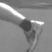
\includegraphics[width=0.17\textwidth]{figures/hog_image.png}
    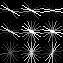
\includegraphics[width=0.17\textwidth]{figures/hog_feature.png}
  \end{center}
  \vspace{-5pt}
  \caption{A example of a patch and  the resulting \gls{hog} cells.}
  \vspace{-10pt}
  \label{fig:hog}
\end{wrapfigure}
\gls{hog} features encode the shape of an object assuming that its shape can be described by the distribution of edge directions. As the name already states we want to look at the gradients of the image at different orientations. We compute the horizontal and vertical gradients from the relative luminance of the original image, using the standard weighted channel contributions. To get the spatial localization we split the image into small regions called cells. For each cell we compute the histogram, which is just an $1d$ vector containing the gradients over a fixed set of angles in that cell. Next we group these cells into larger overlapping blocks. The blocks are used to normalize the contained histograms. This introduces better invariance to illumination and edge contrast. As the blocks are overlapping, each cell will appear multiple times in the output but under different normalization. For normalization we use the L2-norm followed by clipping \citep{lowe_distinctive_2004}.

\subsection{Training}
We collect $1000$ samples of augmented samples, using the same method as described in \treft{sec:pipeline:training:augment}. For all samples we compute the \gls{hog} features using the settings as in \citep{dalal_histograms_2005}. In \citet{felzenszwalb_object_2010} their model consists of multiple parts each described by its own \gls{hog} features. Because we will only train for small parts we describe each sample by only one \gls{hog} descriptor at one scale. Using the set of balanced positive and negative samples we train a linear \gls{svm}.
\clearpage
\subsection{Testing}
The testing pipeline should be as similar as possible to the novel method. To use the same box generation, density calculation and \gls{nms} as in \treft{sec:pipeline:eval}, we need a map of class probability predictions as input. Sliding a window over the images and computing the \gls{hog} features for all positions in the image is rather inefficient. Instead we compute the \gls{hog} descriptors for the whole image and classify a window that is slided over the feature map. The \gls{svm} returns the predicted class (background \textit{vs} foreground), and the scores are aggregated for all windows to build the needed probability map. Although it is not useful to train a multi-scale classifier for our small training samples, we have to take differently scaled test objects into account. Thus we test on multiple scales. Because the \gls{svm} needs a fixed shape, the same number of \gls{hog} blocks, as input to predict their class, we change the \gls{hog} parameters for the different scales. For windows half the size we also halve the width of each \gls{hog} cell, thus resulting in the same number of blocks per window.

\clearpage
\section{Detection results}
\label{sec:results:results}
\begin{figure}[htb]
    \setlength\tabcolsep{0pt}
    \renewcommand{\arraystretch}{0}
    \begin{tabular}{ccccccc}
      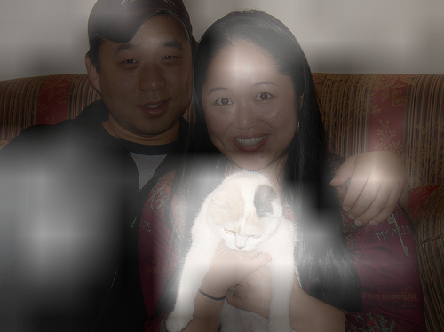
\includegraphics[height=1.8cm]{figures/hm_examples/1s_2008_002067} &
      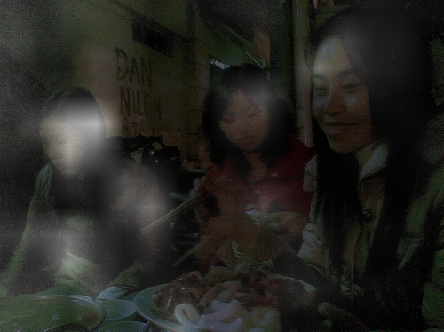
\includegraphics[height=1.8cm]{figures/hm_examples/1s_2009_004323} &
      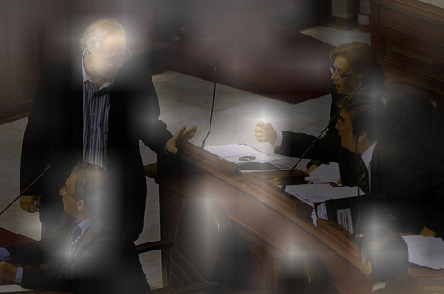
\includegraphics[height=1.8cm]{figures/hm_examples/1s_2009_004784} &
      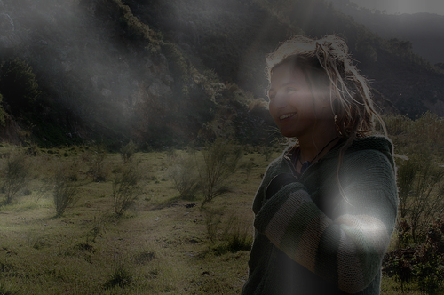
\includegraphics[height=1.8cm]{figures/hm_examples/1s_2009_005222} &
      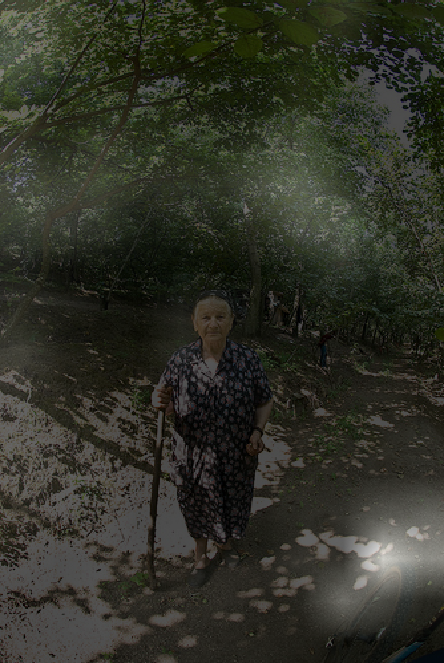
\includegraphics[height=1.8cm]{figures/hm_examples/1s_2009_002715} &
      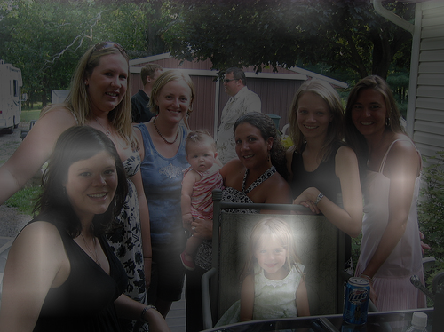
\includegraphics[height=1.8cm]{figures/hm_examples/1s_2010_005967} \\
      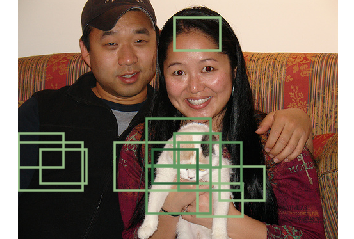
\includegraphics[height=1.8cm]{figures/hm_examples/1s_bbox_2008_002067} &
      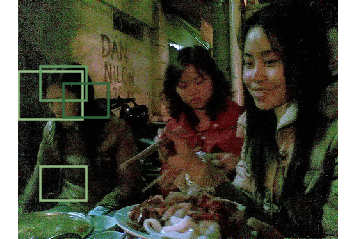
\includegraphics[height=1.8cm]{figures/hm_examples/1s_bbox_2009_004323} &
      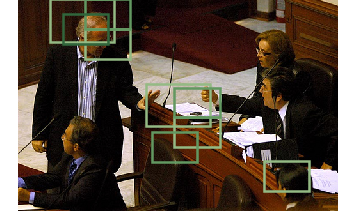
\includegraphics[height=1.8cm]{figures/hm_examples/1s_bbox_2009_004784} &
      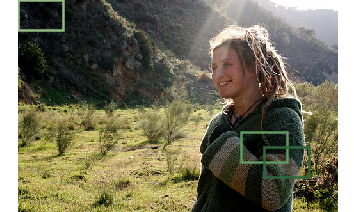
\includegraphics[height=1.8cm]{figures/hm_examples/1s_bbox_2009_005222} &
      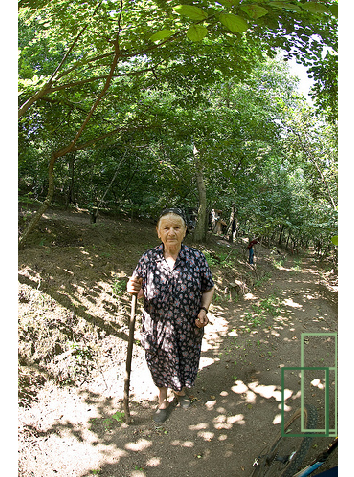
\includegraphics[height=1.8cm]{figures/hm_examples/1s_bbox_2009_002715} &
      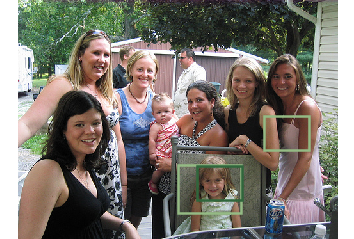
\includegraphics[height=1.8cm]{figures/hm_examples/1s_bbox_2010_005967} \\[3pt]

      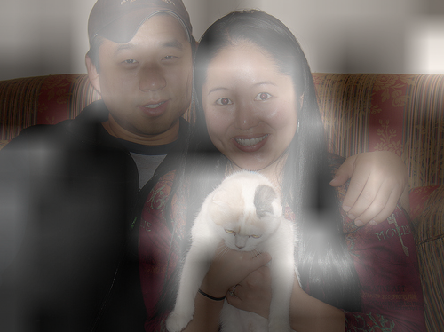
\includegraphics[height=1.8cm]{figures/hm_examples/50s_2008_002067} &
      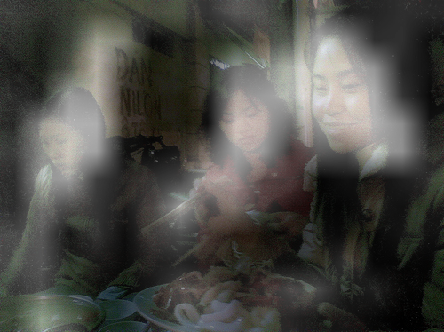
\includegraphics[height=1.8cm]{figures/hm_examples/50s_2009_004323} &
      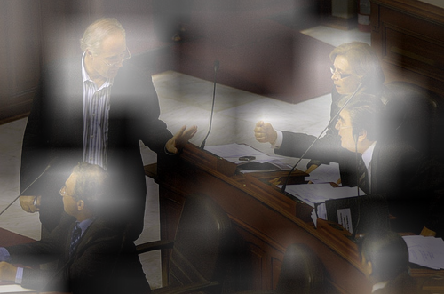
\includegraphics[height=1.8cm]{figures/hm_examples/50s_2009_004784} &
      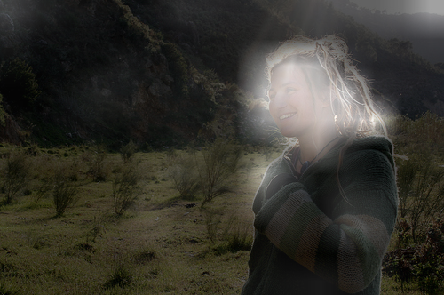
\includegraphics[height=1.8cm]{figures/hm_examples/50s_2009_005222} &
      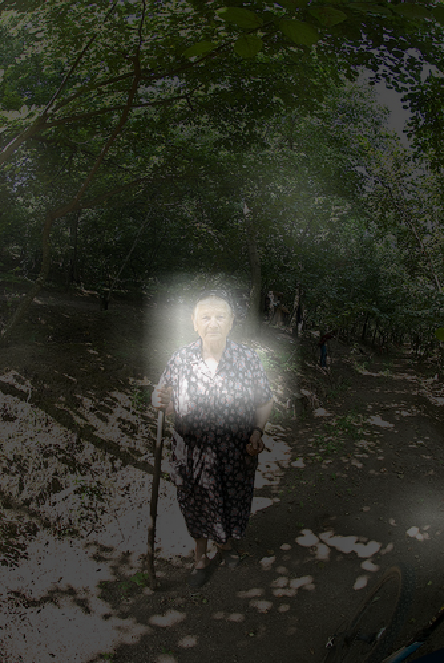
\includegraphics[height=1.8cm]{figures/hm_examples/50s_2009_002715} &
      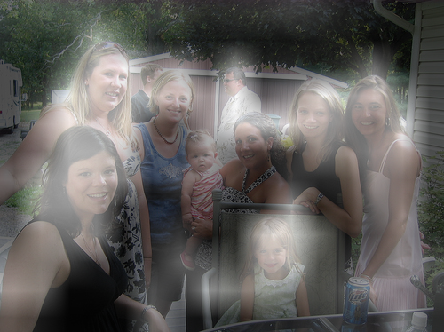
\includegraphics[height=1.8cm]{figures/hm_examples/50s_2010_005967} \\
      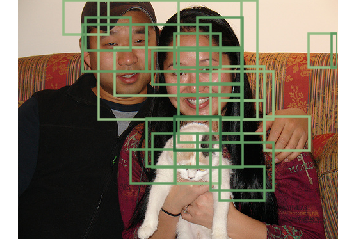
\includegraphics[height=1.8cm]{figures/hm_examples/50s_bbox_2008_002067} &
      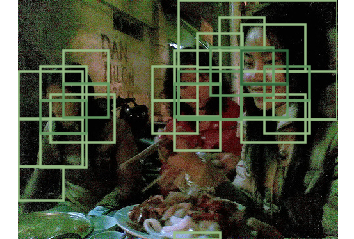
\includegraphics[height=1.8cm]{figures/hm_examples/50s_bbox_2009_004323} &
      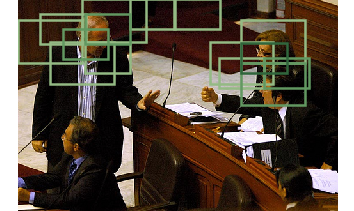
\includegraphics[height=1.8cm]{figures/hm_examples/50s_bbox_2009_004784} &
      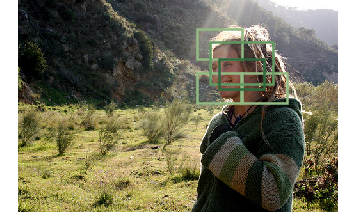
\includegraphics[height=1.8cm]{figures/hm_examples/50s_bbox_2009_005222} &
      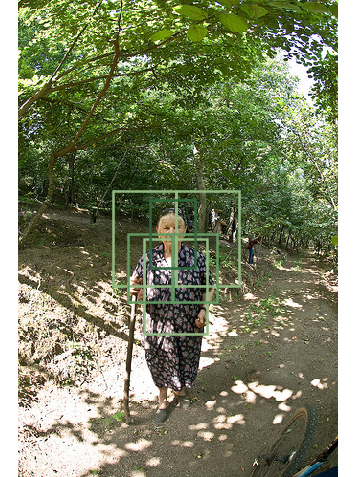
\includegraphics[height=1.8cm]{figures/hm_examples/50s_bbox_2009_002715} &
      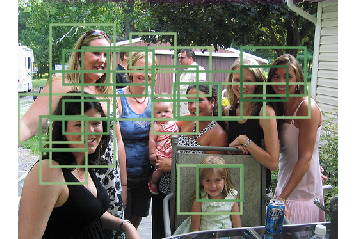
\includegraphics[height=1.8cm]{figures/hm_examples/50s_bbox_2010_005967}

    \end{tabular}
	\caption{Examples from \code{person\_hair}: Top detections are from a run with 1 sample, bottom detections are from a run with 50 samples. Note how the 50 sampled network detects more variations of the parts while the other one does not. Also note how both networks miss-detect the cats head as human hair.}
  \label{fig:hm_examples}
\end{figure}
We test the pipeline for the class-parts combinations $(c,p)$ listed in appendix \ref{sec:appendix:combos}, using the cascade scheme described in \treft{sec:results:repeat}. To evaluate the detection we collect all predicted bounding boxes for all images and their scores.

For a summary of test results see \figreft{fig:auc_heatmap}. We clearly see the correlation between set size and the success in testing. Training with only one sample returns the worst results, by distance, with a mean \gls{auc} over all parts and all runs of 0.72. With increasing set size the test results saturate quickly. The mean \gls{auc} for all larger set sizes lie inside a range of only 0.03. That may be explainable with our training settings, which are designed for fast training and has no time to incorporate a high number of examples into the representation learning.\TODO{add baseline comparsion}

Besides the anticipated correlation between set size and test success, we also show the correlation between different object parts and the success in quickly learning their representation. An example for this difference is given in \figreft{fig:pr_example}. Training on human hair was one of the more successful experiments while training on human necks does not return a useful classifier. The difference can be explained by the amount of discriminating structure a part has to offer. While necks most of the time are very small mostly contrast-less and structure-less patches, hair has a distinguishable surface and therefore more recognizable visual features.

\begin{figure}
  \begin{tabular}{cc}
    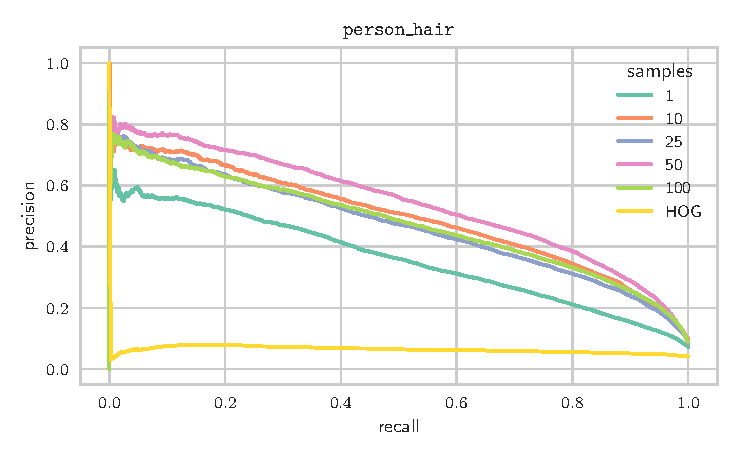
\includegraphics[width=0.47\textwidth]{figures/build/person_hair_precs_recs.pdf} &
    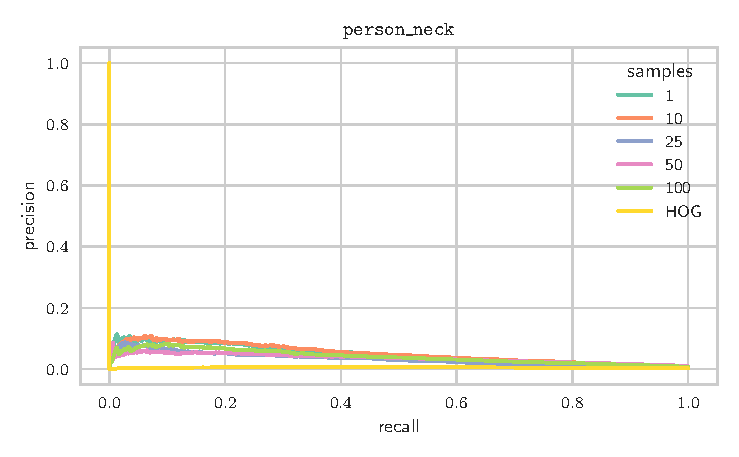
\includegraphics[width=0.47\textwidth]{figures/build/person_neck_precs_recs.pdf}
  \end{tabular}
  \caption{Precision-Recall curves for two parts. \code{person\_hair} on the left as an successful example and \code{person\_neck} as an example for an utterly failed training. Certainly though we see in both plots the clear separation between different set sizes.}
  \label{fig:pr_example}
\end{figure}

Another potential explanation stems from our training method. We train our classifier not on the pixel-precise masks, that \textsc{Pascal}-Part provide, but on rectangular patches retrieved from the original images around each part. As such a patch of human hair will, most of the time, contain a section of the head underneath. One therefore can expect that the model not only learns the representation of the part itself but also of the surrounding object segments. We see this relation in the quite similar results of \code{person\_hair} and \code{person\_head}. Firstly such spatial relations are only relevant in some cases, and secondly while this may frustrate part-based training in some cases, most of the time spatial relations to semantically related parts are an actual indicator for the searched part. If we search for human hair and find human heads, we also found many instances of human hair.

Furthermore we want to check that the cascade testing scheme was intensive enough to report sufficiently precise results. We calculate the variance of \gls{auc} scores for the different parts and training sizes to verify their precision \fref{fig:auc_var_heatmap}. As we expected the variance drastically decreases with increasing set size, and as such we conclude our testing scheme to be adequate for this random sampling. Even for the 20 times repeated 1 sampled training runs, the variance of \gls{auc} scores remains under 0.02 most of the times.
\begin{figure}[p!h]
    \centering
    %% Creator: Matplotlib, PGF backend
%%
%% To include the figure in your LaTeX document, write
%%   \input{<filename>.pgf}
%%
%% Make sure the required packages are loaded in your preamble
%%   \usepackage{pgf}
%%
%% Figures using additional raster images can only be included by \input if
%% they are in the same directory as the main LaTeX file. For loading figures
%% from other directories you can use the `import` package
%%   \usepackage{import}
%% and then include the figures with
%%   \import{<path to file>}{<filename>.pgf}
%%
%% Matplotlib used the following preamble
%%   \usepackage[utf8x]{inputenc}
%%   \usepackage[T1]{fontenc}
%%
\begingroup%
\makeatletter%
\begin{pgfpicture}%
\pgfpathrectangle{\pgfpointorigin}{\pgfqpoint{5.307713in}{6.232660in}}%
\pgfusepath{use as bounding box, clip}%
\begin{pgfscope}%
\pgfsetbuttcap%
\pgfsetmiterjoin%
\definecolor{currentfill}{rgb}{1.000000,1.000000,1.000000}%
\pgfsetfillcolor{currentfill}%
\pgfsetlinewidth{0.000000pt}%
\definecolor{currentstroke}{rgb}{1.000000,1.000000,1.000000}%
\pgfsetstrokecolor{currentstroke}%
\pgfsetdash{}{0pt}%
\pgfpathmoveto{\pgfqpoint{0.000000in}{0.000000in}}%
\pgfpathlineto{\pgfqpoint{5.307713in}{0.000000in}}%
\pgfpathlineto{\pgfqpoint{5.307713in}{6.232660in}}%
\pgfpathlineto{\pgfqpoint{0.000000in}{6.232660in}}%
\pgfpathclose%
\pgfusepath{fill}%
\end{pgfscope}%
\begin{pgfscope}%
\pgfsetbuttcap%
\pgfsetmiterjoin%
\definecolor{currentfill}{rgb}{1.000000,1.000000,1.000000}%
\pgfsetfillcolor{currentfill}%
\pgfsetlinewidth{0.000000pt}%
\definecolor{currentstroke}{rgb}{0.000000,0.000000,0.000000}%
\pgfsetstrokecolor{currentstroke}%
\pgfsetstrokeopacity{0.000000}%
\pgfsetdash{}{0pt}%
\pgfpathmoveto{\pgfqpoint{1.535693in}{0.322448in}}%
\pgfpathlineto{\pgfqpoint{5.163713in}{0.322448in}}%
\pgfpathlineto{\pgfqpoint{5.163713in}{6.088660in}}%
\pgfpathlineto{\pgfqpoint{1.535693in}{6.088660in}}%
\pgfpathclose%
\pgfusepath{fill}%
\end{pgfscope}%
\begin{pgfscope}%
\definecolor{textcolor}{rgb}{0.150000,0.150000,0.150000}%
\pgfsetstrokecolor{textcolor}%
\pgfsetfillcolor{textcolor}%
\pgftext[x=1.898495in,y=0.244670in,,top]{\color{textcolor}\sffamily\fontsize{8.000000}{9.600000}\selectfont 1}%
\end{pgfscope}%
\begin{pgfscope}%
\definecolor{textcolor}{rgb}{0.150000,0.150000,0.150000}%
\pgfsetstrokecolor{textcolor}%
\pgfsetfillcolor{textcolor}%
\pgftext[x=2.624099in,y=0.244670in,,top]{\color{textcolor}\sffamily\fontsize{8.000000}{9.600000}\selectfont 10}%
\end{pgfscope}%
\begin{pgfscope}%
\definecolor{textcolor}{rgb}{0.150000,0.150000,0.150000}%
\pgfsetstrokecolor{textcolor}%
\pgfsetfillcolor{textcolor}%
\pgftext[x=3.349703in,y=0.244670in,,top]{\color{textcolor}\sffamily\fontsize{8.000000}{9.600000}\selectfont 25}%
\end{pgfscope}%
\begin{pgfscope}%
\definecolor{textcolor}{rgb}{0.150000,0.150000,0.150000}%
\pgfsetstrokecolor{textcolor}%
\pgfsetfillcolor{textcolor}%
\pgftext[x=4.075307in,y=0.244670in,,top]{\color{textcolor}\sffamily\fontsize{8.000000}{9.600000}\selectfont 50}%
\end{pgfscope}%
\begin{pgfscope}%
\definecolor{textcolor}{rgb}{0.150000,0.150000,0.150000}%
\pgfsetstrokecolor{textcolor}%
\pgfsetfillcolor{textcolor}%
\pgftext[x=4.800911in,y=0.244670in,,top]{\color{textcolor}\sffamily\fontsize{8.000000}{9.600000}\selectfont 100}%
\end{pgfscope}%
\begin{pgfscope}%
\definecolor{textcolor}{rgb}{0.150000,0.150000,0.150000}%
\pgfsetstrokecolor{textcolor}%
\pgfsetfillcolor{textcolor}%
\pgftext[x=1.184834in,y=0.403042in,left,base]{\color{textcolor}\sffamily\fontsize{8.000000}{9.600000}\selectfont Mean}%
\end{pgfscope}%
\begin{pgfscope}%
\definecolor{textcolor}{rgb}{0.150000,0.150000,0.150000}%
\pgfsetstrokecolor{textcolor}%
\pgfsetfillcolor{textcolor}%
\pgftext[x=0.650705in,y=0.643301in,left,base]{\color{textcolor}\sffamily\fontsize{8.000000}{9.600000}\selectfont train\_hfrontside}%
\end{pgfscope}%
\begin{pgfscope}%
\definecolor{textcolor}{rgb}{0.150000,0.150000,0.150000}%
\pgfsetstrokecolor{textcolor}%
\pgfsetfillcolor{textcolor}%
\pgftext[x=0.906353in,y=0.883560in,left,base]{\color{textcolor}\sffamily\fontsize{8.000000}{9.600000}\selectfont train\_head}%
\end{pgfscope}%
\begin{pgfscope}%
\definecolor{textcolor}{rgb}{0.150000,0.150000,0.150000}%
\pgfsetstrokecolor{textcolor}%
\pgfsetfillcolor{textcolor}%
\pgftext[x=0.855825in,y=1.123818in,left,base]{\color{textcolor}\sffamily\fontsize{8.000000}{9.600000}\selectfont train\_coach}%
\end{pgfscope}%
\begin{pgfscope}%
\definecolor{textcolor}{rgb}{0.150000,0.150000,0.150000}%
\pgfsetstrokecolor{textcolor}%
\pgfsetfillcolor{textcolor}%
\pgftext[x=0.545522in,y=1.364077in,left,base]{\color{textcolor}\sffamily\fontsize{8.000000}{9.600000}\selectfont pottedplant\_plant}%
\end{pgfscope}%
\begin{pgfscope}%
\definecolor{textcolor}{rgb}{0.150000,0.150000,0.150000}%
\pgfsetstrokecolor{textcolor}%
\pgfsetfillcolor{textcolor}%
\pgftext[x=0.801016in,y=1.609659in,left,base]{\color{textcolor}\sffamily\fontsize{8.000000}{9.600000}\selectfont person\_torso}%
\end{pgfscope}%
\begin{pgfscope}%
\definecolor{textcolor}{rgb}{0.150000,0.150000,0.150000}%
\pgfsetstrokecolor{textcolor}%
\pgfsetfillcolor{textcolor}%
\pgftext[x=0.820417in,y=1.844595in,left,base]{\color{textcolor}\sffamily\fontsize{8.000000}{9.600000}\selectfont person\_neck}%
\end{pgfscope}%
\begin{pgfscope}%
\definecolor{textcolor}{rgb}{0.150000,0.150000,0.150000}%
\pgfsetstrokecolor{textcolor}%
\pgfsetfillcolor{textcolor}%
\pgftext[x=0.404623in,y=2.084854in,left,base]{\color{textcolor}\sffamily\fontsize{8.000000}{9.600000}\selectfont person\_lhand\_rhand}%
\end{pgfscope}%
\begin{pgfscope}%
\definecolor{textcolor}{rgb}{0.150000,0.150000,0.150000}%
\pgfsetstrokecolor{textcolor}%
\pgfsetfillcolor{textcolor}%
\pgftext[x=0.483693in,y=2.325113in,left,base]{\color{textcolor}\sffamily\fontsize{8.000000}{9.600000}\selectfont person\_lfoot\_rfoot}%
\end{pgfscope}%
\begin{pgfscope}%
\definecolor{textcolor}{rgb}{0.150000,0.150000,0.150000}%
\pgfsetstrokecolor{textcolor}%
\pgfsetfillcolor{textcolor}%
\pgftext[x=0.591306in,y=2.565372in,left,base]{\color{textcolor}\sffamily\fontsize{8.000000}{9.600000}\selectfont person\_lear\_rear}%
\end{pgfscope}%
\begin{pgfscope}%
\definecolor{textcolor}{rgb}{0.150000,0.150000,0.150000}%
\pgfsetstrokecolor{textcolor}%
\pgfsetfillcolor{textcolor}%
\pgftext[x=0.812895in,y=2.805630in,left,base]{\color{textcolor}\sffamily\fontsize{8.000000}{9.600000}\selectfont person\_head}%
\end{pgfscope}%
\begin{pgfscope}%
\definecolor{textcolor}{rgb}{0.150000,0.150000,0.150000}%
\pgfsetstrokecolor{textcolor}%
\pgfsetfillcolor{textcolor}%
\pgftext[x=0.857830in,y=3.045889in,left,base]{\color{textcolor}\sffamily\fontsize{8.000000}{9.600000}\selectfont person\_hair}%
\end{pgfscope}%
\begin{pgfscope}%
\definecolor{textcolor}{rgb}{0.150000,0.150000,0.150000}%
\pgfsetstrokecolor{textcolor}%
\pgfsetfillcolor{textcolor}%
\pgftext[x=0.144000in,y=3.286148in,left,base]{\color{textcolor}\sffamily\fontsize{8.000000}{9.600000}\selectfont motorbike\_bwheel\_fwheel}%
\end{pgfscope}%
\begin{pgfscope}%
\definecolor{textcolor}{rgb}{0.150000,0.150000,0.150000}%
\pgfsetstrokecolor{textcolor}%
\pgfsetfillcolor{textcolor}%
\pgftext[x=0.217362in,y=3.526407in,left,base]{\color{textcolor}\sffamily\fontsize{8.000000}{9.600000}\selectfont cow\_sheep\_lhorn\_rhorn}%
\end{pgfscope}%
\begin{pgfscope}%
\definecolor{textcolor}{rgb}{0.150000,0.150000,0.150000}%
\pgfsetstrokecolor{textcolor}%
\pgfsetfillcolor{textcolor}%
\pgftext[x=1.000658in,y=3.766666in,left,base]{\color{textcolor}\sffamily\fontsize{8.000000}{9.600000}\selectfont car\_door}%
\end{pgfscope}%
\begin{pgfscope}%
\definecolor{textcolor}{rgb}{0.150000,0.150000,0.150000}%
\pgfsetstrokecolor{textcolor}%
\pgfsetfillcolor{textcolor}%
\pgftext[x=0.178791in,y=4.006925in,left,base]{\color{textcolor}\sffamily\fontsize{8.000000}{9.600000}\selectfont bus\_car\_bliplate\_fliplate}%
\end{pgfscope}%
\begin{pgfscope}%
\definecolor{textcolor}{rgb}{0.150000,0.150000,0.150000}%
\pgfsetstrokecolor{textcolor}%
\pgfsetfillcolor{textcolor}%
\pgftext[x=0.835189in,y=4.247183in,left,base]{\color{textcolor}\sffamily\fontsize{8.000000}{9.600000}\selectfont bottle\_body}%
\end{pgfscope}%
\begin{pgfscope}%
\definecolor{textcolor}{rgb}{0.150000,0.150000,0.150000}%
\pgfsetstrokecolor{textcolor}%
\pgfsetfillcolor{textcolor}%
\pgftext[x=1.020136in,y=4.487442in,left,base]{\color{textcolor}\sffamily\fontsize{8.000000}{9.600000}\selectfont bird\_tail}%
\end{pgfscope}%
\begin{pgfscope}%
\definecolor{textcolor}{rgb}{0.150000,0.150000,0.150000}%
\pgfsetstrokecolor{textcolor}%
\pgfsetfillcolor{textcolor}%
\pgftext[x=0.558058in,y=4.727701in,left,base]{\color{textcolor}\sffamily\fontsize{8.000000}{9.600000}\selectfont bird\_lwing\_rwing}%
\end{pgfscope}%
\begin{pgfscope}%
\definecolor{textcolor}{rgb}{0.150000,0.150000,0.150000}%
\pgfsetstrokecolor{textcolor}%
\pgfsetfillcolor{textcolor}%
\pgftext[x=0.944730in,y=4.967960in,left,base]{\color{textcolor}\sffamily\fontsize{8.000000}{9.600000}\selectfont bird\_head}%
\end{pgfscope}%
\begin{pgfscope}%
\definecolor{textcolor}{rgb}{0.150000,0.150000,0.150000}%
\pgfsetstrokecolor{textcolor}%
\pgfsetfillcolor{textcolor}%
\pgftext[x=0.944730in,y=5.208219in,left,base]{\color{textcolor}\sffamily\fontsize{8.000000}{9.600000}\selectfont bird\_beak}%
\end{pgfscope}%
\begin{pgfscope}%
\definecolor{textcolor}{rgb}{0.150000,0.150000,0.150000}%
\pgfsetstrokecolor{textcolor}%
\pgfsetfillcolor{textcolor}%
\pgftext[x=0.302333in,y=5.448478in,left,base]{\color{textcolor}\sffamily\fontsize{8.000000}{9.600000}\selectfont bicycle\_bwheel\_fwheel}%
\end{pgfscope}%
\begin{pgfscope}%
\definecolor{textcolor}{rgb}{0.150000,0.150000,0.150000}%
\pgfsetstrokecolor{textcolor}%
\pgfsetfillcolor{textcolor}%
\pgftext[x=0.656876in,y=5.688736in,left,base]{\color{textcolor}\sffamily\fontsize{8.000000}{9.600000}\selectfont aeroplane\_stern}%
\end{pgfscope}%
\begin{pgfscope}%
\definecolor{textcolor}{rgb}{0.150000,0.150000,0.150000}%
\pgfsetstrokecolor{textcolor}%
\pgfsetfillcolor{textcolor}%
\pgftext[x=0.280734in,y=5.928995in,left,base]{\color{textcolor}\sffamily\fontsize{8.000000}{9.600000}\selectfont aeroplane\_lwing\_rwing}%
\end{pgfscope}%
\begin{pgfscope}%
\pgfpathrectangle{\pgfqpoint{1.535693in}{0.322448in}}{\pgfqpoint{3.628020in}{5.766212in}} %
\pgfusepath{clip}%
\pgfsetbuttcap%
\pgfsetroundjoin%
\definecolor{currentfill}{rgb}{0.590934,0.737671,0.527775}%
\pgfsetfillcolor{currentfill}%
\pgfsetlinewidth{0.000000pt}%
\definecolor{currentstroke}{rgb}{1.000000,1.000000,1.000000}%
\pgfsetstrokecolor{currentstroke}%
\pgfsetdash{}{0pt}%
\pgfpathmoveto{\pgfqpoint{1.535693in}{0.322448in}}%
\pgfpathlineto{\pgfqpoint{2.261297in}{0.322448in}}%
\pgfpathlineto{\pgfqpoint{2.261297in}{0.562706in}}%
\pgfpathlineto{\pgfqpoint{1.535693in}{0.562706in}}%
\pgfpathlineto{\pgfqpoint{1.535693in}{0.322448in}}%
\pgfusepath{fill}%
\end{pgfscope}%
\begin{pgfscope}%
\pgfpathrectangle{\pgfqpoint{1.535693in}{0.322448in}}{\pgfqpoint{3.628020in}{5.766212in}} %
\pgfusepath{clip}%
\pgfsetbuttcap%
\pgfsetroundjoin%
\definecolor{currentfill}{rgb}{0.412288,0.617543,0.397417}%
\pgfsetfillcolor{currentfill}%
\pgfsetlinewidth{0.000000pt}%
\definecolor{currentstroke}{rgb}{1.000000,1.000000,1.000000}%
\pgfsetstrokecolor{currentstroke}%
\pgfsetdash{}{0pt}%
\pgfpathmoveto{\pgfqpoint{2.261297in}{0.322448in}}%
\pgfpathlineto{\pgfqpoint{2.986901in}{0.322448in}}%
\pgfpathlineto{\pgfqpoint{2.986901in}{0.562706in}}%
\pgfpathlineto{\pgfqpoint{2.261297in}{0.562706in}}%
\pgfpathlineto{\pgfqpoint{2.261297in}{0.322448in}}%
\pgfusepath{fill}%
\end{pgfscope}%
\begin{pgfscope}%
\pgfpathrectangle{\pgfqpoint{1.535693in}{0.322448in}}{\pgfqpoint{3.628020in}{5.766212in}} %
\pgfusepath{clip}%
\pgfsetbuttcap%
\pgfsetroundjoin%
\definecolor{currentfill}{rgb}{0.390531,0.600670,0.382428}%
\pgfsetfillcolor{currentfill}%
\pgfsetlinewidth{0.000000pt}%
\definecolor{currentstroke}{rgb}{1.000000,1.000000,1.000000}%
\pgfsetstrokecolor{currentstroke}%
\pgfsetdash{}{0pt}%
\pgfpathmoveto{\pgfqpoint{2.986901in}{0.322448in}}%
\pgfpathlineto{\pgfqpoint{3.712505in}{0.322448in}}%
\pgfpathlineto{\pgfqpoint{3.712505in}{0.562706in}}%
\pgfpathlineto{\pgfqpoint{2.986901in}{0.562706in}}%
\pgfpathlineto{\pgfqpoint{2.986901in}{0.322448in}}%
\pgfusepath{fill}%
\end{pgfscope}%
\begin{pgfscope}%
\pgfpathrectangle{\pgfqpoint{1.535693in}{0.322448in}}{\pgfqpoint{3.628020in}{5.766212in}} %
\pgfusepath{clip}%
\pgfsetbuttcap%
\pgfsetroundjoin%
\definecolor{currentfill}{rgb}{0.381813,0.593723,0.376436}%
\pgfsetfillcolor{currentfill}%
\pgfsetlinewidth{0.000000pt}%
\definecolor{currentstroke}{rgb}{1.000000,1.000000,1.000000}%
\pgfsetstrokecolor{currentstroke}%
\pgfsetdash{}{0pt}%
\pgfpathmoveto{\pgfqpoint{3.712505in}{0.322448in}}%
\pgfpathlineto{\pgfqpoint{4.438109in}{0.322448in}}%
\pgfpathlineto{\pgfqpoint{4.438109in}{0.562706in}}%
\pgfpathlineto{\pgfqpoint{3.712505in}{0.562706in}}%
\pgfpathlineto{\pgfqpoint{3.712505in}{0.322448in}}%
\pgfusepath{fill}%
\end{pgfscope}%
\begin{pgfscope}%
\pgfpathrectangle{\pgfqpoint{1.535693in}{0.322448in}}{\pgfqpoint{3.628020in}{5.766212in}} %
\pgfusepath{clip}%
\pgfsetbuttcap%
\pgfsetroundjoin%
\definecolor{currentfill}{rgb}{0.377452,0.590206,0.373439}%
\pgfsetfillcolor{currentfill}%
\pgfsetlinewidth{0.000000pt}%
\definecolor{currentstroke}{rgb}{1.000000,1.000000,1.000000}%
\pgfsetstrokecolor{currentstroke}%
\pgfsetdash{}{0pt}%
\pgfpathmoveto{\pgfqpoint{4.438109in}{0.322448in}}%
\pgfpathlineto{\pgfqpoint{5.163713in}{0.322448in}}%
\pgfpathlineto{\pgfqpoint{5.163713in}{0.562706in}}%
\pgfpathlineto{\pgfqpoint{4.438109in}{0.562706in}}%
\pgfpathlineto{\pgfqpoint{4.438109in}{0.322448in}}%
\pgfusepath{fill}%
\end{pgfscope}%
\begin{pgfscope}%
\pgfpathrectangle{\pgfqpoint{1.535693in}{0.322448in}}{\pgfqpoint{3.628020in}{5.766212in}} %
\pgfusepath{clip}%
\pgfsetbuttcap%
\pgfsetroundjoin%
\definecolor{currentfill}{rgb}{0.515548,0.690222,0.470524}%
\pgfsetfillcolor{currentfill}%
\pgfsetlinewidth{0.000000pt}%
\definecolor{currentstroke}{rgb}{1.000000,1.000000,1.000000}%
\pgfsetstrokecolor{currentstroke}%
\pgfsetdash{}{0pt}%
\pgfpathmoveto{\pgfqpoint{1.535693in}{0.562706in}}%
\pgfpathlineto{\pgfqpoint{2.261297in}{0.562706in}}%
\pgfpathlineto{\pgfqpoint{2.261297in}{0.802965in}}%
\pgfpathlineto{\pgfqpoint{1.535693in}{0.802965in}}%
\pgfpathlineto{\pgfqpoint{1.535693in}{0.562706in}}%
\pgfusepath{fill}%
\end{pgfscope}%
\begin{pgfscope}%
\pgfpathrectangle{\pgfqpoint{1.535693in}{0.322448in}}{\pgfqpoint{3.628020in}{5.766212in}} %
\pgfusepath{clip}%
\pgfsetbuttcap%
\pgfsetroundjoin%
\definecolor{currentfill}{rgb}{0.346883,0.564708,0.352416}%
\pgfsetfillcolor{currentfill}%
\pgfsetlinewidth{0.000000pt}%
\definecolor{currentstroke}{rgb}{1.000000,1.000000,1.000000}%
\pgfsetstrokecolor{currentstroke}%
\pgfsetdash{}{0pt}%
\pgfpathmoveto{\pgfqpoint{2.261297in}{0.562706in}}%
\pgfpathlineto{\pgfqpoint{2.986901in}{0.562706in}}%
\pgfpathlineto{\pgfqpoint{2.986901in}{0.802965in}}%
\pgfpathlineto{\pgfqpoint{2.261297in}{0.802965in}}%
\pgfpathlineto{\pgfqpoint{2.261297in}{0.562706in}}%
\pgfusepath{fill}%
\end{pgfscope}%
\begin{pgfscope}%
\pgfpathrectangle{\pgfqpoint{1.535693in}{0.322448in}}{\pgfqpoint{3.628020in}{5.766212in}} %
\pgfusepath{clip}%
\pgfsetbuttcap%
\pgfsetroundjoin%
\definecolor{currentfill}{rgb}{0.342512,0.560933,0.349402}%
\pgfsetfillcolor{currentfill}%
\pgfsetlinewidth{0.000000pt}%
\definecolor{currentstroke}{rgb}{1.000000,1.000000,1.000000}%
\pgfsetstrokecolor{currentstroke}%
\pgfsetdash{}{0pt}%
\pgfpathmoveto{\pgfqpoint{2.986901in}{0.562706in}}%
\pgfpathlineto{\pgfqpoint{3.712505in}{0.562706in}}%
\pgfpathlineto{\pgfqpoint{3.712505in}{0.802965in}}%
\pgfpathlineto{\pgfqpoint{2.986901in}{0.802965in}}%
\pgfpathlineto{\pgfqpoint{2.986901in}{0.562706in}}%
\pgfusepath{fill}%
\end{pgfscope}%
\begin{pgfscope}%
\pgfpathrectangle{\pgfqpoint{1.535693in}{0.322448in}}{\pgfqpoint{3.628020in}{5.766212in}} %
\pgfusepath{clip}%
\pgfsetbuttcap%
\pgfsetroundjoin%
\definecolor{currentfill}{rgb}{0.359992,0.575829,0.361440}%
\pgfsetfillcolor{currentfill}%
\pgfsetlinewidth{0.000000pt}%
\definecolor{currentstroke}{rgb}{1.000000,1.000000,1.000000}%
\pgfsetstrokecolor{currentstroke}%
\pgfsetdash{}{0pt}%
\pgfpathmoveto{\pgfqpoint{3.712505in}{0.562706in}}%
\pgfpathlineto{\pgfqpoint{4.438109in}{0.562706in}}%
\pgfpathlineto{\pgfqpoint{4.438109in}{0.802965in}}%
\pgfpathlineto{\pgfqpoint{3.712505in}{0.802965in}}%
\pgfpathlineto{\pgfqpoint{3.712505in}{0.562706in}}%
\pgfusepath{fill}%
\end{pgfscope}%
\begin{pgfscope}%
\pgfpathrectangle{\pgfqpoint{1.535693in}{0.322448in}}{\pgfqpoint{3.628020in}{5.766212in}} %
\pgfusepath{clip}%
\pgfsetbuttcap%
\pgfsetroundjoin%
\definecolor{currentfill}{rgb}{0.359992,0.575829,0.361440}%
\pgfsetfillcolor{currentfill}%
\pgfsetlinewidth{0.000000pt}%
\definecolor{currentstroke}{rgb}{1.000000,1.000000,1.000000}%
\pgfsetstrokecolor{currentstroke}%
\pgfsetdash{}{0pt}%
\pgfpathmoveto{\pgfqpoint{4.438109in}{0.562706in}}%
\pgfpathlineto{\pgfqpoint{5.163713in}{0.562706in}}%
\pgfpathlineto{\pgfqpoint{5.163713in}{0.802965in}}%
\pgfpathlineto{\pgfqpoint{4.438109in}{0.802965in}}%
\pgfpathlineto{\pgfqpoint{4.438109in}{0.562706in}}%
\pgfusepath{fill}%
\end{pgfscope}%
\begin{pgfscope}%
\pgfpathrectangle{\pgfqpoint{1.535693in}{0.322448in}}{\pgfqpoint{3.628020in}{5.766212in}} %
\pgfusepath{clip}%
\pgfsetbuttcap%
\pgfsetroundjoin%
\definecolor{currentfill}{rgb}{0.285645,0.508428,0.309642}%
\pgfsetfillcolor{currentfill}%
\pgfsetlinewidth{0.000000pt}%
\definecolor{currentstroke}{rgb}{1.000000,1.000000,1.000000}%
\pgfsetstrokecolor{currentstroke}%
\pgfsetdash{}{0pt}%
\pgfpathmoveto{\pgfqpoint{1.535693in}{0.802965in}}%
\pgfpathlineto{\pgfqpoint{2.261297in}{0.802965in}}%
\pgfpathlineto{\pgfqpoint{2.261297in}{1.043224in}}%
\pgfpathlineto{\pgfqpoint{1.535693in}{1.043224in}}%
\pgfpathlineto{\pgfqpoint{1.535693in}{0.802965in}}%
\pgfusepath{fill}%
\end{pgfscope}%
\begin{pgfscope}%
\pgfpathrectangle{\pgfqpoint{1.535693in}{0.322448in}}{\pgfqpoint{3.628020in}{5.766212in}} %
\pgfusepath{clip}%
\pgfsetbuttcap%
\pgfsetroundjoin%
\definecolor{currentfill}{rgb}{0.298770,0.521154,0.318941}%
\pgfsetfillcolor{currentfill}%
\pgfsetlinewidth{0.000000pt}%
\definecolor{currentstroke}{rgb}{1.000000,1.000000,1.000000}%
\pgfsetstrokecolor{currentstroke}%
\pgfsetdash{}{0pt}%
\pgfpathmoveto{\pgfqpoint{2.261297in}{0.802965in}}%
\pgfpathlineto{\pgfqpoint{2.986901in}{0.802965in}}%
\pgfpathlineto{\pgfqpoint{2.986901in}{1.043224in}}%
\pgfpathlineto{\pgfqpoint{2.261297in}{1.043224in}}%
\pgfpathlineto{\pgfqpoint{2.261297in}{0.802965in}}%
\pgfusepath{fill}%
\end{pgfscope}%
\begin{pgfscope}%
\pgfpathrectangle{\pgfqpoint{1.535693in}{0.322448in}}{\pgfqpoint{3.628020in}{5.766212in}} %
\pgfusepath{clip}%
\pgfsetbuttcap%
\pgfsetroundjoin%
\definecolor{currentfill}{rgb}{0.303146,0.525309,0.322021}%
\pgfsetfillcolor{currentfill}%
\pgfsetlinewidth{0.000000pt}%
\definecolor{currentstroke}{rgb}{1.000000,1.000000,1.000000}%
\pgfsetstrokecolor{currentstroke}%
\pgfsetdash{}{0pt}%
\pgfpathmoveto{\pgfqpoint{2.986901in}{0.802965in}}%
\pgfpathlineto{\pgfqpoint{3.712505in}{0.802965in}}%
\pgfpathlineto{\pgfqpoint{3.712505in}{1.043224in}}%
\pgfpathlineto{\pgfqpoint{2.986901in}{1.043224in}}%
\pgfpathlineto{\pgfqpoint{2.986901in}{0.802965in}}%
\pgfusepath{fill}%
\end{pgfscope}%
\begin{pgfscope}%
\pgfpathrectangle{\pgfqpoint{1.535693in}{0.322448in}}{\pgfqpoint{3.628020in}{5.766212in}} %
\pgfusepath{clip}%
\pgfsetbuttcap%
\pgfsetroundjoin%
\definecolor{currentfill}{rgb}{0.338140,0.557124,0.346383}%
\pgfsetfillcolor{currentfill}%
\pgfsetlinewidth{0.000000pt}%
\definecolor{currentstroke}{rgb}{1.000000,1.000000,1.000000}%
\pgfsetstrokecolor{currentstroke}%
\pgfsetdash{}{0pt}%
\pgfpathmoveto{\pgfqpoint{3.712505in}{0.802965in}}%
\pgfpathlineto{\pgfqpoint{4.438109in}{0.802965in}}%
\pgfpathlineto{\pgfqpoint{4.438109in}{1.043224in}}%
\pgfpathlineto{\pgfqpoint{3.712505in}{1.043224in}}%
\pgfpathlineto{\pgfqpoint{3.712505in}{0.802965in}}%
\pgfusepath{fill}%
\end{pgfscope}%
\begin{pgfscope}%
\pgfpathrectangle{\pgfqpoint{1.535693in}{0.322448in}}{\pgfqpoint{3.628020in}{5.766212in}} %
\pgfusepath{clip}%
\pgfsetbuttcap%
\pgfsetroundjoin%
\definecolor{currentfill}{rgb}{0.329394,0.549398,0.340330}%
\pgfsetfillcolor{currentfill}%
\pgfsetlinewidth{0.000000pt}%
\definecolor{currentstroke}{rgb}{1.000000,1.000000,1.000000}%
\pgfsetstrokecolor{currentstroke}%
\pgfsetdash{}{0pt}%
\pgfpathmoveto{\pgfqpoint{4.438109in}{0.802965in}}%
\pgfpathlineto{\pgfqpoint{5.163713in}{0.802965in}}%
\pgfpathlineto{\pgfqpoint{5.163713in}{1.043224in}}%
\pgfpathlineto{\pgfqpoint{4.438109in}{1.043224in}}%
\pgfpathlineto{\pgfqpoint{4.438109in}{0.802965in}}%
\pgfusepath{fill}%
\end{pgfscope}%
\begin{pgfscope}%
\pgfpathrectangle{\pgfqpoint{1.535693in}{0.322448in}}{\pgfqpoint{3.628020in}{5.766212in}} %
\pgfusepath{clip}%
\pgfsetbuttcap%
\pgfsetroundjoin%
\definecolor{currentfill}{rgb}{0.706479,0.805466,0.626151}%
\pgfsetfillcolor{currentfill}%
\pgfsetlinewidth{0.000000pt}%
\definecolor{currentstroke}{rgb}{1.000000,1.000000,1.000000}%
\pgfsetstrokecolor{currentstroke}%
\pgfsetdash{}{0pt}%
\pgfpathmoveto{\pgfqpoint{1.535693in}{1.043224in}}%
\pgfpathlineto{\pgfqpoint{2.261297in}{1.043224in}}%
\pgfpathlineto{\pgfqpoint{2.261297in}{1.283483in}}%
\pgfpathlineto{\pgfqpoint{1.535693in}{1.283483in}}%
\pgfpathlineto{\pgfqpoint{1.535693in}{1.043224in}}%
\pgfusepath{fill}%
\end{pgfscope}%
\begin{pgfscope}%
\pgfpathrectangle{\pgfqpoint{1.535693in}{0.322448in}}{\pgfqpoint{3.628020in}{5.766212in}} %
\pgfusepath{clip}%
\pgfsetbuttcap%
\pgfsetroundjoin%
\definecolor{currentfill}{rgb}{0.611438,0.750022,0.544165}%
\pgfsetfillcolor{currentfill}%
\pgfsetlinewidth{0.000000pt}%
\definecolor{currentstroke}{rgb}{1.000000,1.000000,1.000000}%
\pgfsetstrokecolor{currentstroke}%
\pgfsetdash{}{0pt}%
\pgfpathmoveto{\pgfqpoint{2.261297in}{1.043224in}}%
\pgfpathlineto{\pgfqpoint{2.986901in}{1.043224in}}%
\pgfpathlineto{\pgfqpoint{2.986901in}{1.283483in}}%
\pgfpathlineto{\pgfqpoint{2.261297in}{1.283483in}}%
\pgfpathlineto{\pgfqpoint{2.261297in}{1.043224in}}%
\pgfusepath{fill}%
\end{pgfscope}%
\begin{pgfscope}%
\pgfpathrectangle{\pgfqpoint{1.535693in}{0.322448in}}{\pgfqpoint{3.628020in}{5.766212in}} %
\pgfusepath{clip}%
\pgfsetbuttcap%
\pgfsetroundjoin%
\definecolor{currentfill}{rgb}{0.570225,0.724986,0.511606}%
\pgfsetfillcolor{currentfill}%
\pgfsetlinewidth{0.000000pt}%
\definecolor{currentstroke}{rgb}{1.000000,1.000000,1.000000}%
\pgfsetstrokecolor{currentstroke}%
\pgfsetdash{}{0pt}%
\pgfpathmoveto{\pgfqpoint{2.986901in}{1.043224in}}%
\pgfpathlineto{\pgfqpoint{3.712505in}{1.043224in}}%
\pgfpathlineto{\pgfqpoint{3.712505in}{1.283483in}}%
\pgfpathlineto{\pgfqpoint{2.986901in}{1.283483in}}%
\pgfpathlineto{\pgfqpoint{2.986901in}{1.043224in}}%
\pgfusepath{fill}%
\end{pgfscope}%
\begin{pgfscope}%
\pgfpathrectangle{\pgfqpoint{1.535693in}{0.322448in}}{\pgfqpoint{3.628020in}{5.766212in}} %
\pgfusepath{clip}%
\pgfsetbuttcap%
\pgfsetroundjoin%
\definecolor{currentfill}{rgb}{0.570225,0.724986,0.511606}%
\pgfsetfillcolor{currentfill}%
\pgfsetlinewidth{0.000000pt}%
\definecolor{currentstroke}{rgb}{1.000000,1.000000,1.000000}%
\pgfsetstrokecolor{currentstroke}%
\pgfsetdash{}{0pt}%
\pgfpathmoveto{\pgfqpoint{3.712505in}{1.043224in}}%
\pgfpathlineto{\pgfqpoint{4.438109in}{1.043224in}}%
\pgfpathlineto{\pgfqpoint{4.438109in}{1.283483in}}%
\pgfpathlineto{\pgfqpoint{3.712505in}{1.283483in}}%
\pgfpathlineto{\pgfqpoint{3.712505in}{1.043224in}}%
\pgfusepath{fill}%
\end{pgfscope}%
\begin{pgfscope}%
\pgfpathrectangle{\pgfqpoint{1.535693in}{0.322448in}}{\pgfqpoint{3.628020in}{5.766212in}} %
\pgfusepath{clip}%
\pgfsetbuttcap%
\pgfsetroundjoin%
\definecolor{currentfill}{rgb}{0.566060,0.722406,0.508398}%
\pgfsetfillcolor{currentfill}%
\pgfsetlinewidth{0.000000pt}%
\definecolor{currentstroke}{rgb}{1.000000,1.000000,1.000000}%
\pgfsetstrokecolor{currentstroke}%
\pgfsetdash{}{0pt}%
\pgfpathmoveto{\pgfqpoint{4.438109in}{1.043224in}}%
\pgfpathlineto{\pgfqpoint{5.163713in}{1.043224in}}%
\pgfpathlineto{\pgfqpoint{5.163713in}{1.283483in}}%
\pgfpathlineto{\pgfqpoint{4.438109in}{1.283483in}}%
\pgfpathlineto{\pgfqpoint{4.438109in}{1.043224in}}%
\pgfusepath{fill}%
\end{pgfscope}%
\begin{pgfscope}%
\pgfpathrectangle{\pgfqpoint{1.535693in}{0.322448in}}{\pgfqpoint{3.628020in}{5.766212in}} %
\pgfusepath{clip}%
\pgfsetbuttcap%
\pgfsetroundjoin%
\definecolor{currentfill}{rgb}{0.561888,0.719811,0.505199}%
\pgfsetfillcolor{currentfill}%
\pgfsetlinewidth{0.000000pt}%
\definecolor{currentstroke}{rgb}{1.000000,1.000000,1.000000}%
\pgfsetstrokecolor{currentstroke}%
\pgfsetdash{}{0pt}%
\pgfpathmoveto{\pgfqpoint{1.535693in}{1.283483in}}%
\pgfpathlineto{\pgfqpoint{2.261297in}{1.283483in}}%
\pgfpathlineto{\pgfqpoint{2.261297in}{1.523742in}}%
\pgfpathlineto{\pgfqpoint{1.535693in}{1.523742in}}%
\pgfpathlineto{\pgfqpoint{1.535693in}{1.283483in}}%
\pgfusepath{fill}%
\end{pgfscope}%
\begin{pgfscope}%
\pgfpathrectangle{\pgfqpoint{1.535693in}{0.322448in}}{\pgfqpoint{3.628020in}{5.766212in}} %
\pgfusepath{clip}%
\pgfsetbuttcap%
\pgfsetroundjoin%
\definecolor{currentfill}{rgb}{0.399240,0.607502,0.388421}%
\pgfsetfillcolor{currentfill}%
\pgfsetlinewidth{0.000000pt}%
\definecolor{currentstroke}{rgb}{1.000000,1.000000,1.000000}%
\pgfsetstrokecolor{currentstroke}%
\pgfsetdash{}{0pt}%
\pgfpathmoveto{\pgfqpoint{2.261297in}{1.283483in}}%
\pgfpathlineto{\pgfqpoint{2.986901in}{1.283483in}}%
\pgfpathlineto{\pgfqpoint{2.986901in}{1.523742in}}%
\pgfpathlineto{\pgfqpoint{2.261297in}{1.523742in}}%
\pgfpathlineto{\pgfqpoint{2.261297in}{1.283483in}}%
\pgfusepath{fill}%
\end{pgfscope}%
\begin{pgfscope}%
\pgfpathrectangle{\pgfqpoint{1.535693in}{0.322448in}}{\pgfqpoint{3.628020in}{5.766212in}} %
\pgfusepath{clip}%
\pgfsetbuttcap%
\pgfsetroundjoin%
\definecolor{currentfill}{rgb}{0.359992,0.575829,0.361440}%
\pgfsetfillcolor{currentfill}%
\pgfsetlinewidth{0.000000pt}%
\definecolor{currentstroke}{rgb}{1.000000,1.000000,1.000000}%
\pgfsetstrokecolor{currentstroke}%
\pgfsetdash{}{0pt}%
\pgfpathmoveto{\pgfqpoint{2.986901in}{1.283483in}}%
\pgfpathlineto{\pgfqpoint{3.712505in}{1.283483in}}%
\pgfpathlineto{\pgfqpoint{3.712505in}{1.523742in}}%
\pgfpathlineto{\pgfqpoint{2.986901in}{1.523742in}}%
\pgfpathlineto{\pgfqpoint{2.986901in}{1.283483in}}%
\pgfusepath{fill}%
\end{pgfscope}%
\begin{pgfscope}%
\pgfpathrectangle{\pgfqpoint{1.535693in}{0.322448in}}{\pgfqpoint{3.628020in}{5.766212in}} %
\pgfusepath{clip}%
\pgfsetbuttcap%
\pgfsetroundjoin%
\definecolor{currentfill}{rgb}{0.346883,0.564708,0.352416}%
\pgfsetfillcolor{currentfill}%
\pgfsetlinewidth{0.000000pt}%
\definecolor{currentstroke}{rgb}{1.000000,1.000000,1.000000}%
\pgfsetstrokecolor{currentstroke}%
\pgfsetdash{}{0pt}%
\pgfpathmoveto{\pgfqpoint{3.712505in}{1.283483in}}%
\pgfpathlineto{\pgfqpoint{4.438109in}{1.283483in}}%
\pgfpathlineto{\pgfqpoint{4.438109in}{1.523742in}}%
\pgfpathlineto{\pgfqpoint{3.712505in}{1.523742in}}%
\pgfpathlineto{\pgfqpoint{3.712505in}{1.283483in}}%
\pgfusepath{fill}%
\end{pgfscope}%
\begin{pgfscope}%
\pgfpathrectangle{\pgfqpoint{1.535693in}{0.322448in}}{\pgfqpoint{3.628020in}{5.766212in}} %
\pgfusepath{clip}%
\pgfsetbuttcap%
\pgfsetroundjoin%
\definecolor{currentfill}{rgb}{0.333767,0.553279,0.343359}%
\pgfsetfillcolor{currentfill}%
\pgfsetlinewidth{0.000000pt}%
\definecolor{currentstroke}{rgb}{1.000000,1.000000,1.000000}%
\pgfsetstrokecolor{currentstroke}%
\pgfsetdash{}{0pt}%
\pgfpathmoveto{\pgfqpoint{4.438109in}{1.283483in}}%
\pgfpathlineto{\pgfqpoint{5.163713in}{1.283483in}}%
\pgfpathlineto{\pgfqpoint{5.163713in}{1.523742in}}%
\pgfpathlineto{\pgfqpoint{4.438109in}{1.523742in}}%
\pgfpathlineto{\pgfqpoint{4.438109in}{1.283483in}}%
\pgfusepath{fill}%
\end{pgfscope}%
\begin{pgfscope}%
\pgfpathrectangle{\pgfqpoint{1.535693in}{0.322448in}}{\pgfqpoint{3.628020in}{5.766212in}} %
\pgfusepath{clip}%
\pgfsetbuttcap%
\pgfsetroundjoin%
\definecolor{currentfill}{rgb}{0.845429,0.886933,0.771307}%
\pgfsetfillcolor{currentfill}%
\pgfsetlinewidth{0.000000pt}%
\definecolor{currentstroke}{rgb}{1.000000,1.000000,1.000000}%
\pgfsetstrokecolor{currentstroke}%
\pgfsetdash{}{0pt}%
\pgfpathmoveto{\pgfqpoint{1.535693in}{1.523742in}}%
\pgfpathlineto{\pgfqpoint{2.261297in}{1.523742in}}%
\pgfpathlineto{\pgfqpoint{2.261297in}{1.764001in}}%
\pgfpathlineto{\pgfqpoint{1.535693in}{1.764001in}}%
\pgfpathlineto{\pgfqpoint{1.535693in}{1.523742in}}%
\pgfusepath{fill}%
\end{pgfscope}%
\begin{pgfscope}%
\pgfpathrectangle{\pgfqpoint{1.535693in}{0.322448in}}{\pgfqpoint{3.628020in}{5.766212in}} %
\pgfusepath{clip}%
\pgfsetbuttcap%
\pgfsetroundjoin%
\definecolor{currentfill}{rgb}{0.481402,0.667359,0.445838}%
\pgfsetfillcolor{currentfill}%
\pgfsetlinewidth{0.000000pt}%
\definecolor{currentstroke}{rgb}{1.000000,1.000000,1.000000}%
\pgfsetstrokecolor{currentstroke}%
\pgfsetdash{}{0pt}%
\pgfpathmoveto{\pgfqpoint{2.261297in}{1.523742in}}%
\pgfpathlineto{\pgfqpoint{2.986901in}{1.523742in}}%
\pgfpathlineto{\pgfqpoint{2.986901in}{1.764001in}}%
\pgfpathlineto{\pgfqpoint{2.261297in}{1.764001in}}%
\pgfpathlineto{\pgfqpoint{2.261297in}{1.523742in}}%
\pgfusepath{fill}%
\end{pgfscope}%
\begin{pgfscope}%
\pgfpathrectangle{\pgfqpoint{1.535693in}{0.322448in}}{\pgfqpoint{3.628020in}{5.766212in}} %
\pgfusepath{clip}%
\pgfsetbuttcap%
\pgfsetroundjoin%
\definecolor{currentfill}{rgb}{0.333767,0.553279,0.343359}%
\pgfsetfillcolor{currentfill}%
\pgfsetlinewidth{0.000000pt}%
\definecolor{currentstroke}{rgb}{1.000000,1.000000,1.000000}%
\pgfsetstrokecolor{currentstroke}%
\pgfsetdash{}{0pt}%
\pgfpathmoveto{\pgfqpoint{2.986901in}{1.523742in}}%
\pgfpathlineto{\pgfqpoint{3.712505in}{1.523742in}}%
\pgfpathlineto{\pgfqpoint{3.712505in}{1.764001in}}%
\pgfpathlineto{\pgfqpoint{2.986901in}{1.764001in}}%
\pgfpathlineto{\pgfqpoint{2.986901in}{1.523742in}}%
\pgfusepath{fill}%
\end{pgfscope}%
\begin{pgfscope}%
\pgfpathrectangle{\pgfqpoint{1.535693in}{0.322448in}}{\pgfqpoint{3.628020in}{5.766212in}} %
\pgfusepath{clip}%
\pgfsetbuttcap%
\pgfsetroundjoin%
\definecolor{currentfill}{rgb}{0.386173,0.597211,0.379432}%
\pgfsetfillcolor{currentfill}%
\pgfsetlinewidth{0.000000pt}%
\definecolor{currentstroke}{rgb}{1.000000,1.000000,1.000000}%
\pgfsetstrokecolor{currentstroke}%
\pgfsetdash{}{0pt}%
\pgfpathmoveto{\pgfqpoint{3.712505in}{1.523742in}}%
\pgfpathlineto{\pgfqpoint{4.438109in}{1.523742in}}%
\pgfpathlineto{\pgfqpoint{4.438109in}{1.764001in}}%
\pgfpathlineto{\pgfqpoint{3.712505in}{1.764001in}}%
\pgfpathlineto{\pgfqpoint{3.712505in}{1.523742in}}%
\pgfusepath{fill}%
\end{pgfscope}%
\begin{pgfscope}%
\pgfpathrectangle{\pgfqpoint{1.535693in}{0.322448in}}{\pgfqpoint{3.628020in}{5.766212in}} %
\pgfusepath{clip}%
\pgfsetbuttcap%
\pgfsetroundjoin%
\definecolor{currentfill}{rgb}{0.399240,0.607502,0.388421}%
\pgfsetfillcolor{currentfill}%
\pgfsetlinewidth{0.000000pt}%
\definecolor{currentstroke}{rgb}{1.000000,1.000000,1.000000}%
\pgfsetstrokecolor{currentstroke}%
\pgfsetdash{}{0pt}%
\pgfpathmoveto{\pgfqpoint{4.438109in}{1.523742in}}%
\pgfpathlineto{\pgfqpoint{5.163713in}{1.523742in}}%
\pgfpathlineto{\pgfqpoint{5.163713in}{1.764001in}}%
\pgfpathlineto{\pgfqpoint{4.438109in}{1.764001in}}%
\pgfpathlineto{\pgfqpoint{4.438109in}{1.523742in}}%
\pgfusepath{fill}%
\end{pgfscope}%
\begin{pgfscope}%
\pgfpathrectangle{\pgfqpoint{1.535693in}{0.322448in}}{\pgfqpoint{3.628020in}{5.766212in}} %
\pgfusepath{clip}%
\pgfsetbuttcap%
\pgfsetroundjoin%
\definecolor{currentfill}{rgb}{0.329394,0.549398,0.340330}%
\pgfsetfillcolor{currentfill}%
\pgfsetlinewidth{0.000000pt}%
\definecolor{currentstroke}{rgb}{1.000000,1.000000,1.000000}%
\pgfsetstrokecolor{currentstroke}%
\pgfsetdash{}{0pt}%
\pgfpathmoveto{\pgfqpoint{1.535693in}{1.764001in}}%
\pgfpathlineto{\pgfqpoint{2.261297in}{1.764001in}}%
\pgfpathlineto{\pgfqpoint{2.261297in}{2.004259in}}%
\pgfpathlineto{\pgfqpoint{1.535693in}{2.004259in}}%
\pgfpathlineto{\pgfqpoint{1.535693in}{1.764001in}}%
\pgfusepath{fill}%
\end{pgfscope}%
\begin{pgfscope}%
\pgfpathrectangle{\pgfqpoint{1.535693in}{0.322448in}}{\pgfqpoint{3.628020in}{5.766212in}} %
\pgfusepath{clip}%
\pgfsetbuttcap%
\pgfsetroundjoin%
\definecolor{currentfill}{rgb}{0.338140,0.557124,0.346383}%
\pgfsetfillcolor{currentfill}%
\pgfsetlinewidth{0.000000pt}%
\definecolor{currentstroke}{rgb}{1.000000,1.000000,1.000000}%
\pgfsetstrokecolor{currentstroke}%
\pgfsetdash{}{0pt}%
\pgfpathmoveto{\pgfqpoint{2.261297in}{1.764001in}}%
\pgfpathlineto{\pgfqpoint{2.986901in}{1.764001in}}%
\pgfpathlineto{\pgfqpoint{2.986901in}{2.004259in}}%
\pgfpathlineto{\pgfqpoint{2.261297in}{2.004259in}}%
\pgfpathlineto{\pgfqpoint{2.261297in}{1.764001in}}%
\pgfusepath{fill}%
\end{pgfscope}%
\begin{pgfscope}%
\pgfpathrectangle{\pgfqpoint{1.535693in}{0.322448in}}{\pgfqpoint{3.628020in}{5.766212in}} %
\pgfusepath{clip}%
\pgfsetbuttcap%
\pgfsetroundjoin%
\definecolor{currentfill}{rgb}{0.429648,0.630565,0.409438}%
\pgfsetfillcolor{currentfill}%
\pgfsetlinewidth{0.000000pt}%
\definecolor{currentstroke}{rgb}{1.000000,1.000000,1.000000}%
\pgfsetstrokecolor{currentstroke}%
\pgfsetdash{}{0pt}%
\pgfpathmoveto{\pgfqpoint{2.986901in}{1.764001in}}%
\pgfpathlineto{\pgfqpoint{3.712505in}{1.764001in}}%
\pgfpathlineto{\pgfqpoint{3.712505in}{2.004259in}}%
\pgfpathlineto{\pgfqpoint{2.986901in}{2.004259in}}%
\pgfpathlineto{\pgfqpoint{2.986901in}{1.764001in}}%
\pgfusepath{fill}%
\end{pgfscope}%
\begin{pgfscope}%
\pgfpathrectangle{\pgfqpoint{1.535693in}{0.322448in}}{\pgfqpoint{3.628020in}{5.766212in}} %
\pgfusepath{clip}%
\pgfsetbuttcap%
\pgfsetroundjoin%
\definecolor{currentfill}{rgb}{0.377452,0.590206,0.373439}%
\pgfsetfillcolor{currentfill}%
\pgfsetlinewidth{0.000000pt}%
\definecolor{currentstroke}{rgb}{1.000000,1.000000,1.000000}%
\pgfsetstrokecolor{currentstroke}%
\pgfsetdash{}{0pt}%
\pgfpathmoveto{\pgfqpoint{3.712505in}{1.764001in}}%
\pgfpathlineto{\pgfqpoint{4.438109in}{1.764001in}}%
\pgfpathlineto{\pgfqpoint{4.438109in}{2.004259in}}%
\pgfpathlineto{\pgfqpoint{3.712505in}{2.004259in}}%
\pgfpathlineto{\pgfqpoint{3.712505in}{1.764001in}}%
\pgfusepath{fill}%
\end{pgfscope}%
\begin{pgfscope}%
\pgfpathrectangle{\pgfqpoint{1.535693in}{0.322448in}}{\pgfqpoint{3.628020in}{5.766212in}} %
\pgfusepath{clip}%
\pgfsetbuttcap%
\pgfsetroundjoin%
\definecolor{currentfill}{rgb}{0.377452,0.590206,0.373439}%
\pgfsetfillcolor{currentfill}%
\pgfsetlinewidth{0.000000pt}%
\definecolor{currentstroke}{rgb}{1.000000,1.000000,1.000000}%
\pgfsetstrokecolor{currentstroke}%
\pgfsetdash{}{0pt}%
\pgfpathmoveto{\pgfqpoint{4.438109in}{1.764001in}}%
\pgfpathlineto{\pgfqpoint{5.163713in}{1.764001in}}%
\pgfpathlineto{\pgfqpoint{5.163713in}{2.004259in}}%
\pgfpathlineto{\pgfqpoint{4.438109in}{2.004259in}}%
\pgfpathlineto{\pgfqpoint{4.438109in}{1.764001in}}%
\pgfusepath{fill}%
\end{pgfscope}%
\begin{pgfscope}%
\pgfpathrectangle{\pgfqpoint{1.535693in}{0.322448in}}{\pgfqpoint{3.628020in}{5.766212in}} %
\pgfusepath{clip}%
\pgfsetbuttcap%
\pgfsetroundjoin%
\definecolor{currentfill}{rgb}{0.675480,0.787603,0.598197}%
\pgfsetfillcolor{currentfill}%
\pgfsetlinewidth{0.000000pt}%
\definecolor{currentstroke}{rgb}{1.000000,1.000000,1.000000}%
\pgfsetstrokecolor{currentstroke}%
\pgfsetdash{}{0pt}%
\pgfpathmoveto{\pgfqpoint{1.535693in}{2.004259in}}%
\pgfpathlineto{\pgfqpoint{2.261297in}{2.004259in}}%
\pgfpathlineto{\pgfqpoint{2.261297in}{2.244518in}}%
\pgfpathlineto{\pgfqpoint{1.535693in}{2.244518in}}%
\pgfpathlineto{\pgfqpoint{1.535693in}{2.004259in}}%
\pgfusepath{fill}%
\end{pgfscope}%
\begin{pgfscope}%
\pgfpathrectangle{\pgfqpoint{1.535693in}{0.322448in}}{\pgfqpoint{3.628020in}{5.766212in}} %
\pgfusepath{clip}%
\pgfsetbuttcap%
\pgfsetroundjoin%
\definecolor{currentfill}{rgb}{0.307521,0.529423,0.325092}%
\pgfsetfillcolor{currentfill}%
\pgfsetlinewidth{0.000000pt}%
\definecolor{currentstroke}{rgb}{1.000000,1.000000,1.000000}%
\pgfsetstrokecolor{currentstroke}%
\pgfsetdash{}{0pt}%
\pgfpathmoveto{\pgfqpoint{2.261297in}{2.004259in}}%
\pgfpathlineto{\pgfqpoint{2.986901in}{2.004259in}}%
\pgfpathlineto{\pgfqpoint{2.986901in}{2.244518in}}%
\pgfpathlineto{\pgfqpoint{2.261297in}{2.244518in}}%
\pgfpathlineto{\pgfqpoint{2.261297in}{2.004259in}}%
\pgfusepath{fill}%
\end{pgfscope}%
\begin{pgfscope}%
\pgfpathrectangle{\pgfqpoint{1.535693in}{0.322448in}}{\pgfqpoint{3.628020in}{5.766212in}} %
\pgfusepath{clip}%
\pgfsetbuttcap%
\pgfsetroundjoin%
\definecolor{currentfill}{rgb}{0.338140,0.557124,0.346383}%
\pgfsetfillcolor{currentfill}%
\pgfsetlinewidth{0.000000pt}%
\definecolor{currentstroke}{rgb}{1.000000,1.000000,1.000000}%
\pgfsetstrokecolor{currentstroke}%
\pgfsetdash{}{0pt}%
\pgfpathmoveto{\pgfqpoint{2.986901in}{2.004259in}}%
\pgfpathlineto{\pgfqpoint{3.712505in}{2.004259in}}%
\pgfpathlineto{\pgfqpoint{3.712505in}{2.244518in}}%
\pgfpathlineto{\pgfqpoint{2.986901in}{2.244518in}}%
\pgfpathlineto{\pgfqpoint{2.986901in}{2.004259in}}%
\pgfusepath{fill}%
\end{pgfscope}%
\begin{pgfscope}%
\pgfpathrectangle{\pgfqpoint{1.535693in}{0.322448in}}{\pgfqpoint{3.628020in}{5.766212in}} %
\pgfusepath{clip}%
\pgfsetbuttcap%
\pgfsetroundjoin%
\definecolor{currentfill}{rgb}{0.368725,0.583080,0.367443}%
\pgfsetfillcolor{currentfill}%
\pgfsetlinewidth{0.000000pt}%
\definecolor{currentstroke}{rgb}{1.000000,1.000000,1.000000}%
\pgfsetstrokecolor{currentstroke}%
\pgfsetdash{}{0pt}%
\pgfpathmoveto{\pgfqpoint{3.712505in}{2.004259in}}%
\pgfpathlineto{\pgfqpoint{4.438109in}{2.004259in}}%
\pgfpathlineto{\pgfqpoint{4.438109in}{2.244518in}}%
\pgfpathlineto{\pgfqpoint{3.712505in}{2.244518in}}%
\pgfpathlineto{\pgfqpoint{3.712505in}{2.004259in}}%
\pgfusepath{fill}%
\end{pgfscope}%
\begin{pgfscope}%
\pgfpathrectangle{\pgfqpoint{1.535693in}{0.322448in}}{\pgfqpoint{3.628020in}{5.766212in}} %
\pgfusepath{clip}%
\pgfsetbuttcap%
\pgfsetroundjoin%
\definecolor{currentfill}{rgb}{0.377452,0.590206,0.373439}%
\pgfsetfillcolor{currentfill}%
\pgfsetlinewidth{0.000000pt}%
\definecolor{currentstroke}{rgb}{1.000000,1.000000,1.000000}%
\pgfsetstrokecolor{currentstroke}%
\pgfsetdash{}{0pt}%
\pgfpathmoveto{\pgfqpoint{4.438109in}{2.004259in}}%
\pgfpathlineto{\pgfqpoint{5.163713in}{2.004259in}}%
\pgfpathlineto{\pgfqpoint{5.163713in}{2.244518in}}%
\pgfpathlineto{\pgfqpoint{4.438109in}{2.244518in}}%
\pgfpathlineto{\pgfqpoint{4.438109in}{2.004259in}}%
\pgfusepath{fill}%
\end{pgfscope}%
\begin{pgfscope}%
\pgfpathrectangle{\pgfqpoint{1.535693in}{0.322448in}}{\pgfqpoint{3.628020in}{5.766212in}} %
\pgfusepath{clip}%
\pgfsetbuttcap%
\pgfsetroundjoin%
\definecolor{currentfill}{rgb}{0.832225,0.878855,0.755777}%
\pgfsetfillcolor{currentfill}%
\pgfsetlinewidth{0.000000pt}%
\definecolor{currentstroke}{rgb}{1.000000,1.000000,1.000000}%
\pgfsetstrokecolor{currentstroke}%
\pgfsetdash{}{0pt}%
\pgfpathmoveto{\pgfqpoint{1.535693in}{2.244518in}}%
\pgfpathlineto{\pgfqpoint{2.261297in}{2.244518in}}%
\pgfpathlineto{\pgfqpoint{2.261297in}{2.484777in}}%
\pgfpathlineto{\pgfqpoint{1.535693in}{2.484777in}}%
\pgfpathlineto{\pgfqpoint{1.535693in}{2.244518in}}%
\pgfusepath{fill}%
\end{pgfscope}%
\begin{pgfscope}%
\pgfpathrectangle{\pgfqpoint{1.535693in}{0.322448in}}{\pgfqpoint{3.628020in}{5.766212in}} %
\pgfusepath{clip}%
\pgfsetbuttcap%
\pgfsetroundjoin%
\definecolor{currentfill}{rgb}{0.429648,0.630565,0.409438}%
\pgfsetfillcolor{currentfill}%
\pgfsetlinewidth{0.000000pt}%
\definecolor{currentstroke}{rgb}{1.000000,1.000000,1.000000}%
\pgfsetstrokecolor{currentstroke}%
\pgfsetdash{}{0pt}%
\pgfpathmoveto{\pgfqpoint{2.261297in}{2.244518in}}%
\pgfpathlineto{\pgfqpoint{2.986901in}{2.244518in}}%
\pgfpathlineto{\pgfqpoint{2.986901in}{2.484777in}}%
\pgfpathlineto{\pgfqpoint{2.261297in}{2.484777in}}%
\pgfpathlineto{\pgfqpoint{2.261297in}{2.244518in}}%
\pgfusepath{fill}%
\end{pgfscope}%
\begin{pgfscope}%
\pgfpathrectangle{\pgfqpoint{1.535693in}{0.322448in}}{\pgfqpoint{3.628020in}{5.766212in}} %
\pgfusepath{clip}%
\pgfsetbuttcap%
\pgfsetroundjoin%
\definecolor{currentfill}{rgb}{0.394887,0.604100,0.385424}%
\pgfsetfillcolor{currentfill}%
\pgfsetlinewidth{0.000000pt}%
\definecolor{currentstroke}{rgb}{1.000000,1.000000,1.000000}%
\pgfsetstrokecolor{currentstroke}%
\pgfsetdash{}{0pt}%
\pgfpathmoveto{\pgfqpoint{2.986901in}{2.244518in}}%
\pgfpathlineto{\pgfqpoint{3.712505in}{2.244518in}}%
\pgfpathlineto{\pgfqpoint{3.712505in}{2.484777in}}%
\pgfpathlineto{\pgfqpoint{2.986901in}{2.484777in}}%
\pgfpathlineto{\pgfqpoint{2.986901in}{2.244518in}}%
\pgfusepath{fill}%
\end{pgfscope}%
\begin{pgfscope}%
\pgfpathrectangle{\pgfqpoint{1.535693in}{0.322448in}}{\pgfqpoint{3.628020in}{5.766212in}} %
\pgfusepath{clip}%
\pgfsetbuttcap%
\pgfsetroundjoin%
\definecolor{currentfill}{rgb}{0.485688,0.670285,0.448902}%
\pgfsetfillcolor{currentfill}%
\pgfsetlinewidth{0.000000pt}%
\definecolor{currentstroke}{rgb}{1.000000,1.000000,1.000000}%
\pgfsetstrokecolor{currentstroke}%
\pgfsetdash{}{0pt}%
\pgfpathmoveto{\pgfqpoint{3.712505in}{2.244518in}}%
\pgfpathlineto{\pgfqpoint{4.438109in}{2.244518in}}%
\pgfpathlineto{\pgfqpoint{4.438109in}{2.484777in}}%
\pgfpathlineto{\pgfqpoint{3.712505in}{2.484777in}}%
\pgfpathlineto{\pgfqpoint{3.712505in}{2.244518in}}%
\pgfusepath{fill}%
\end{pgfscope}%
\begin{pgfscope}%
\pgfpathrectangle{\pgfqpoint{1.535693in}{0.322448in}}{\pgfqpoint{3.628020in}{5.766212in}} %
\pgfusepath{clip}%
\pgfsetbuttcap%
\pgfsetroundjoin%
\definecolor{currentfill}{rgb}{0.536708,0.703919,0.486171}%
\pgfsetfillcolor{currentfill}%
\pgfsetlinewidth{0.000000pt}%
\definecolor{currentstroke}{rgb}{1.000000,1.000000,1.000000}%
\pgfsetstrokecolor{currentstroke}%
\pgfsetdash{}{0pt}%
\pgfpathmoveto{\pgfqpoint{4.438109in}{2.244518in}}%
\pgfpathlineto{\pgfqpoint{5.163713in}{2.244518in}}%
\pgfpathlineto{\pgfqpoint{5.163713in}{2.484777in}}%
\pgfpathlineto{\pgfqpoint{4.438109in}{2.484777in}}%
\pgfpathlineto{\pgfqpoint{4.438109in}{2.244518in}}%
\pgfusepath{fill}%
\end{pgfscope}%
\begin{pgfscope}%
\pgfpathrectangle{\pgfqpoint{1.535693in}{0.322448in}}{\pgfqpoint{3.628020in}{5.766212in}} %
\pgfusepath{clip}%
\pgfsetbuttcap%
\pgfsetroundjoin%
\definecolor{currentfill}{rgb}{0.399240,0.607502,0.388421}%
\pgfsetfillcolor{currentfill}%
\pgfsetlinewidth{0.000000pt}%
\definecolor{currentstroke}{rgb}{1.000000,1.000000,1.000000}%
\pgfsetstrokecolor{currentstroke}%
\pgfsetdash{}{0pt}%
\pgfpathmoveto{\pgfqpoint{1.535693in}{2.484777in}}%
\pgfpathlineto{\pgfqpoint{2.261297in}{2.484777in}}%
\pgfpathlineto{\pgfqpoint{2.261297in}{2.725036in}}%
\pgfpathlineto{\pgfqpoint{1.535693in}{2.725036in}}%
\pgfpathlineto{\pgfqpoint{1.535693in}{2.484777in}}%
\pgfusepath{fill}%
\end{pgfscope}%
\begin{pgfscope}%
\pgfpathrectangle{\pgfqpoint{1.535693in}{0.322448in}}{\pgfqpoint{3.628020in}{5.766212in}} %
\pgfusepath{clip}%
\pgfsetbuttcap%
\pgfsetroundjoin%
\definecolor{currentfill}{rgb}{0.667618,0.783050,0.591307}%
\pgfsetfillcolor{currentfill}%
\pgfsetlinewidth{0.000000pt}%
\definecolor{currentstroke}{rgb}{1.000000,1.000000,1.000000}%
\pgfsetstrokecolor{currentstroke}%
\pgfsetdash{}{0pt}%
\pgfpathmoveto{\pgfqpoint{2.261297in}{2.484777in}}%
\pgfpathlineto{\pgfqpoint{2.986901in}{2.484777in}}%
\pgfpathlineto{\pgfqpoint{2.986901in}{2.725036in}}%
\pgfpathlineto{\pgfqpoint{2.261297in}{2.725036in}}%
\pgfpathlineto{\pgfqpoint{2.261297in}{2.484777in}}%
\pgfusepath{fill}%
\end{pgfscope}%
\begin{pgfscope}%
\pgfpathrectangle{\pgfqpoint{1.535693in}{0.322448in}}{\pgfqpoint{3.628020in}{5.766212in}} %
\pgfusepath{clip}%
\pgfsetbuttcap%
\pgfsetroundjoin%
\definecolor{currentfill}{rgb}{0.623635,0.757283,0.554109}%
\pgfsetfillcolor{currentfill}%
\pgfsetlinewidth{0.000000pt}%
\definecolor{currentstroke}{rgb}{1.000000,1.000000,1.000000}%
\pgfsetstrokecolor{currentstroke}%
\pgfsetdash{}{0pt}%
\pgfpathmoveto{\pgfqpoint{2.986901in}{2.484777in}}%
\pgfpathlineto{\pgfqpoint{3.712505in}{2.484777in}}%
\pgfpathlineto{\pgfqpoint{3.712505in}{2.725036in}}%
\pgfpathlineto{\pgfqpoint{2.986901in}{2.725036in}}%
\pgfpathlineto{\pgfqpoint{2.986901in}{2.484777in}}%
\pgfusepath{fill}%
\end{pgfscope}%
\begin{pgfscope}%
\pgfpathrectangle{\pgfqpoint{1.535693in}{0.322448in}}{\pgfqpoint{3.628020in}{5.766212in}} %
\pgfusepath{clip}%
\pgfsetbuttcap%
\pgfsetroundjoin%
\definecolor{currentfill}{rgb}{0.659712,0.778458,0.584456}%
\pgfsetfillcolor{currentfill}%
\pgfsetlinewidth{0.000000pt}%
\definecolor{currentstroke}{rgb}{1.000000,1.000000,1.000000}%
\pgfsetstrokecolor{currentstroke}%
\pgfsetdash{}{0pt}%
\pgfpathmoveto{\pgfqpoint{3.712505in}{2.484777in}}%
\pgfpathlineto{\pgfqpoint{4.438109in}{2.484777in}}%
\pgfpathlineto{\pgfqpoint{4.438109in}{2.725036in}}%
\pgfpathlineto{\pgfqpoint{3.712505in}{2.725036in}}%
\pgfpathlineto{\pgfqpoint{3.712505in}{2.484777in}}%
\pgfusepath{fill}%
\end{pgfscope}%
\begin{pgfscope}%
\pgfpathrectangle{\pgfqpoint{1.535693in}{0.322448in}}{\pgfqpoint{3.628020in}{5.766212in}} %
\pgfusepath{clip}%
\pgfsetbuttcap%
\pgfsetroundjoin%
\definecolor{currentfill}{rgb}{0.515548,0.690222,0.470524}%
\pgfsetfillcolor{currentfill}%
\pgfsetlinewidth{0.000000pt}%
\definecolor{currentstroke}{rgb}{1.000000,1.000000,1.000000}%
\pgfsetstrokecolor{currentstroke}%
\pgfsetdash{}{0pt}%
\pgfpathmoveto{\pgfqpoint{4.438109in}{2.484777in}}%
\pgfpathlineto{\pgfqpoint{5.163713in}{2.484777in}}%
\pgfpathlineto{\pgfqpoint{5.163713in}{2.725036in}}%
\pgfpathlineto{\pgfqpoint{4.438109in}{2.725036in}}%
\pgfpathlineto{\pgfqpoint{4.438109in}{2.484777in}}%
\pgfusepath{fill}%
\end{pgfscope}%
\begin{pgfscope}%
\pgfpathrectangle{\pgfqpoint{1.535693in}{0.322448in}}{\pgfqpoint{3.628020in}{5.766212in}} %
\pgfusepath{clip}%
\pgfsetbuttcap%
\pgfsetroundjoin%
\definecolor{currentfill}{rgb}{0.747833,0.829234,0.665624}%
\pgfsetfillcolor{currentfill}%
\pgfsetlinewidth{0.000000pt}%
\definecolor{currentstroke}{rgb}{1.000000,1.000000,1.000000}%
\pgfsetstrokecolor{currentstroke}%
\pgfsetdash{}{0pt}%
\pgfpathmoveto{\pgfqpoint{1.535693in}{2.725036in}}%
\pgfpathlineto{\pgfqpoint{2.261297in}{2.725036in}}%
\pgfpathlineto{\pgfqpoint{2.261297in}{2.965295in}}%
\pgfpathlineto{\pgfqpoint{1.535693in}{2.965295in}}%
\pgfpathlineto{\pgfqpoint{1.535693in}{2.725036in}}%
\pgfusepath{fill}%
\end{pgfscope}%
\begin{pgfscope}%
\pgfpathrectangle{\pgfqpoint{1.535693in}{0.322448in}}{\pgfqpoint{3.628020in}{5.766212in}} %
\pgfusepath{clip}%
\pgfsetbuttcap%
\pgfsetroundjoin%
\definecolor{currentfill}{rgb}{0.381813,0.593723,0.376436}%
\pgfsetfillcolor{currentfill}%
\pgfsetlinewidth{0.000000pt}%
\definecolor{currentstroke}{rgb}{1.000000,1.000000,1.000000}%
\pgfsetstrokecolor{currentstroke}%
\pgfsetdash{}{0pt}%
\pgfpathmoveto{\pgfqpoint{2.261297in}{2.725036in}}%
\pgfpathlineto{\pgfqpoint{2.986901in}{2.725036in}}%
\pgfpathlineto{\pgfqpoint{2.986901in}{2.965295in}}%
\pgfpathlineto{\pgfqpoint{2.261297in}{2.965295in}}%
\pgfpathlineto{\pgfqpoint{2.261297in}{2.725036in}}%
\pgfusepath{fill}%
\end{pgfscope}%
\begin{pgfscope}%
\pgfpathrectangle{\pgfqpoint{1.535693in}{0.322448in}}{\pgfqpoint{3.628020in}{5.766212in}} %
\pgfusepath{clip}%
\pgfsetbuttcap%
\pgfsetroundjoin%
\definecolor{currentfill}{rgb}{0.311896,0.533496,0.328154}%
\pgfsetfillcolor{currentfill}%
\pgfsetlinewidth{0.000000pt}%
\definecolor{currentstroke}{rgb}{1.000000,1.000000,1.000000}%
\pgfsetstrokecolor{currentstroke}%
\pgfsetdash{}{0pt}%
\pgfpathmoveto{\pgfqpoint{2.986901in}{2.725036in}}%
\pgfpathlineto{\pgfqpoint{3.712505in}{2.725036in}}%
\pgfpathlineto{\pgfqpoint{3.712505in}{2.965295in}}%
\pgfpathlineto{\pgfqpoint{2.986901in}{2.965295in}}%
\pgfpathlineto{\pgfqpoint{2.986901in}{2.725036in}}%
\pgfusepath{fill}%
\end{pgfscope}%
\begin{pgfscope}%
\pgfpathrectangle{\pgfqpoint{1.535693in}{0.322448in}}{\pgfqpoint{3.628020in}{5.766212in}} %
\pgfusepath{clip}%
\pgfsetbuttcap%
\pgfsetroundjoin%
\definecolor{currentfill}{rgb}{0.276895,0.499719,0.303385}%
\pgfsetfillcolor{currentfill}%
\pgfsetlinewidth{0.000000pt}%
\definecolor{currentstroke}{rgb}{1.000000,1.000000,1.000000}%
\pgfsetstrokecolor{currentstroke}%
\pgfsetdash{}{0pt}%
\pgfpathmoveto{\pgfqpoint{3.712505in}{2.725036in}}%
\pgfpathlineto{\pgfqpoint{4.438109in}{2.725036in}}%
\pgfpathlineto{\pgfqpoint{4.438109in}{2.965295in}}%
\pgfpathlineto{\pgfqpoint{3.712505in}{2.965295in}}%
\pgfpathlineto{\pgfqpoint{3.712505in}{2.725036in}}%
\pgfusepath{fill}%
\end{pgfscope}%
\begin{pgfscope}%
\pgfpathrectangle{\pgfqpoint{1.535693in}{0.322448in}}{\pgfqpoint{3.628020in}{5.766212in}} %
\pgfusepath{clip}%
\pgfsetbuttcap%
\pgfsetroundjoin%
\definecolor{currentfill}{rgb}{0.250654,0.472417,0.284274}%
\pgfsetfillcolor{currentfill}%
\pgfsetlinewidth{0.000000pt}%
\definecolor{currentstroke}{rgb}{1.000000,1.000000,1.000000}%
\pgfsetstrokecolor{currentstroke}%
\pgfsetdash{}{0pt}%
\pgfpathmoveto{\pgfqpoint{4.438109in}{2.725036in}}%
\pgfpathlineto{\pgfqpoint{5.163713in}{2.725036in}}%
\pgfpathlineto{\pgfqpoint{5.163713in}{2.965295in}}%
\pgfpathlineto{\pgfqpoint{4.438109in}{2.965295in}}%
\pgfpathlineto{\pgfqpoint{4.438109in}{2.725036in}}%
\pgfusepath{fill}%
\end{pgfscope}%
\begin{pgfscope}%
\pgfpathrectangle{\pgfqpoint{1.535693in}{0.322448in}}{\pgfqpoint{3.628020in}{5.766212in}} %
\pgfusepath{clip}%
\pgfsetbuttcap%
\pgfsetroundjoin%
\definecolor{currentfill}{rgb}{0.316271,0.537530,0.331208}%
\pgfsetfillcolor{currentfill}%
\pgfsetlinewidth{0.000000pt}%
\definecolor{currentstroke}{rgb}{1.000000,1.000000,1.000000}%
\pgfsetstrokecolor{currentstroke}%
\pgfsetdash{}{0pt}%
\pgfpathmoveto{\pgfqpoint{1.535693in}{2.965295in}}%
\pgfpathlineto{\pgfqpoint{2.261297in}{2.965295in}}%
\pgfpathlineto{\pgfqpoint{2.261297in}{3.205554in}}%
\pgfpathlineto{\pgfqpoint{1.535693in}{3.205554in}}%
\pgfpathlineto{\pgfqpoint{1.535693in}{2.965295in}}%
\pgfusepath{fill}%
\end{pgfscope}%
\begin{pgfscope}%
\pgfpathrectangle{\pgfqpoint{1.535693in}{0.322448in}}{\pgfqpoint{3.628020in}{5.766212in}} %
\pgfusepath{clip}%
\pgfsetbuttcap%
\pgfsetroundjoin%
\definecolor{currentfill}{rgb}{0.263773,0.486297,0.293900}%
\pgfsetfillcolor{currentfill}%
\pgfsetlinewidth{0.000000pt}%
\definecolor{currentstroke}{rgb}{1.000000,1.000000,1.000000}%
\pgfsetstrokecolor{currentstroke}%
\pgfsetdash{}{0pt}%
\pgfpathmoveto{\pgfqpoint{2.261297in}{2.965295in}}%
\pgfpathlineto{\pgfqpoint{2.986901in}{2.965295in}}%
\pgfpathlineto{\pgfqpoint{2.986901in}{3.205554in}}%
\pgfpathlineto{\pgfqpoint{2.261297in}{3.205554in}}%
\pgfpathlineto{\pgfqpoint{2.261297in}{2.965295in}}%
\pgfusepath{fill}%
\end{pgfscope}%
\begin{pgfscope}%
\pgfpathrectangle{\pgfqpoint{1.535693in}{0.322448in}}{\pgfqpoint{3.628020in}{5.766212in}} %
\pgfusepath{clip}%
\pgfsetbuttcap%
\pgfsetroundjoin%
\definecolor{currentfill}{rgb}{0.259399,0.481723,0.290708}%
\pgfsetfillcolor{currentfill}%
\pgfsetlinewidth{0.000000pt}%
\definecolor{currentstroke}{rgb}{1.000000,1.000000,1.000000}%
\pgfsetstrokecolor{currentstroke}%
\pgfsetdash{}{0pt}%
\pgfpathmoveto{\pgfqpoint{2.986901in}{2.965295in}}%
\pgfpathlineto{\pgfqpoint{3.712505in}{2.965295in}}%
\pgfpathlineto{\pgfqpoint{3.712505in}{3.205554in}}%
\pgfpathlineto{\pgfqpoint{2.986901in}{3.205554in}}%
\pgfpathlineto{\pgfqpoint{2.986901in}{2.965295in}}%
\pgfusepath{fill}%
\end{pgfscope}%
\begin{pgfscope}%
\pgfpathrectangle{\pgfqpoint{1.535693in}{0.322448in}}{\pgfqpoint{3.628020in}{5.766212in}} %
\pgfusepath{clip}%
\pgfsetbuttcap%
\pgfsetroundjoin%
\definecolor{currentfill}{rgb}{0.228795,0.448169,0.267853}%
\pgfsetfillcolor{currentfill}%
\pgfsetlinewidth{0.000000pt}%
\definecolor{currentstroke}{rgb}{1.000000,1.000000,1.000000}%
\pgfsetstrokecolor{currentstroke}%
\pgfsetdash{}{0pt}%
\pgfpathmoveto{\pgfqpoint{3.712505in}{2.965295in}}%
\pgfpathlineto{\pgfqpoint{4.438109in}{2.965295in}}%
\pgfpathlineto{\pgfqpoint{4.438109in}{3.205554in}}%
\pgfpathlineto{\pgfqpoint{3.712505in}{3.205554in}}%
\pgfpathlineto{\pgfqpoint{3.712505in}{2.965295in}}%
\pgfusepath{fill}%
\end{pgfscope}%
\begin{pgfscope}%
\pgfpathrectangle{\pgfqpoint{1.535693in}{0.322448in}}{\pgfqpoint{3.628020in}{5.766212in}} %
\pgfusepath{clip}%
\pgfsetbuttcap%
\pgfsetroundjoin%
\definecolor{currentfill}{rgb}{0.255026,0.477097,0.287500}%
\pgfsetfillcolor{currentfill}%
\pgfsetlinewidth{0.000000pt}%
\definecolor{currentstroke}{rgb}{1.000000,1.000000,1.000000}%
\pgfsetstrokecolor{currentstroke}%
\pgfsetdash{}{0pt}%
\pgfpathmoveto{\pgfqpoint{4.438109in}{2.965295in}}%
\pgfpathlineto{\pgfqpoint{5.163713in}{2.965295in}}%
\pgfpathlineto{\pgfqpoint{5.163713in}{3.205554in}}%
\pgfpathlineto{\pgfqpoint{4.438109in}{3.205554in}}%
\pgfpathlineto{\pgfqpoint{4.438109in}{2.965295in}}%
\pgfusepath{fill}%
\end{pgfscope}%
\begin{pgfscope}%
\pgfpathrectangle{\pgfqpoint{1.535693in}{0.322448in}}{\pgfqpoint{3.628020in}{5.766212in}} %
\pgfusepath{clip}%
\pgfsetbuttcap%
\pgfsetroundjoin%
\definecolor{currentfill}{rgb}{0.268147,0.490820,0.297076}%
\pgfsetfillcolor{currentfill}%
\pgfsetlinewidth{0.000000pt}%
\definecolor{currentstroke}{rgb}{1.000000,1.000000,1.000000}%
\pgfsetstrokecolor{currentstroke}%
\pgfsetdash{}{0pt}%
\pgfpathmoveto{\pgfqpoint{1.535693in}{3.205554in}}%
\pgfpathlineto{\pgfqpoint{2.261297in}{3.205554in}}%
\pgfpathlineto{\pgfqpoint{2.261297in}{3.445813in}}%
\pgfpathlineto{\pgfqpoint{1.535693in}{3.445813in}}%
\pgfpathlineto{\pgfqpoint{1.535693in}{3.205554in}}%
\pgfusepath{fill}%
\end{pgfscope}%
\begin{pgfscope}%
\pgfpathrectangle{\pgfqpoint{1.535693in}{0.322448in}}{\pgfqpoint{3.628020in}{5.766212in}} %
\pgfusepath{clip}%
\pgfsetbuttcap%
\pgfsetroundjoin%
\definecolor{currentfill}{rgb}{0.442637,0.640071,0.418483}%
\pgfsetfillcolor{currentfill}%
\pgfsetlinewidth{0.000000pt}%
\definecolor{currentstroke}{rgb}{1.000000,1.000000,1.000000}%
\pgfsetstrokecolor{currentstroke}%
\pgfsetdash{}{0pt}%
\pgfpathmoveto{\pgfqpoint{2.261297in}{3.205554in}}%
\pgfpathlineto{\pgfqpoint{2.986901in}{3.205554in}}%
\pgfpathlineto{\pgfqpoint{2.986901in}{3.445813in}}%
\pgfpathlineto{\pgfqpoint{2.261297in}{3.445813in}}%
\pgfpathlineto{\pgfqpoint{2.261297in}{3.205554in}}%
\pgfusepath{fill}%
\end{pgfscope}%
\begin{pgfscope}%
\pgfpathrectangle{\pgfqpoint{1.535693in}{0.322448in}}{\pgfqpoint{3.628020in}{5.766212in}} %
\pgfusepath{clip}%
\pgfsetbuttcap%
\pgfsetroundjoin%
\definecolor{currentfill}{rgb}{0.429648,0.630565,0.409438}%
\pgfsetfillcolor{currentfill}%
\pgfsetlinewidth{0.000000pt}%
\definecolor{currentstroke}{rgb}{1.000000,1.000000,1.000000}%
\pgfsetstrokecolor{currentstroke}%
\pgfsetdash{}{0pt}%
\pgfpathmoveto{\pgfqpoint{2.986901in}{3.205554in}}%
\pgfpathlineto{\pgfqpoint{3.712505in}{3.205554in}}%
\pgfpathlineto{\pgfqpoint{3.712505in}{3.445813in}}%
\pgfpathlineto{\pgfqpoint{2.986901in}{3.445813in}}%
\pgfpathlineto{\pgfqpoint{2.986901in}{3.205554in}}%
\pgfusepath{fill}%
\end{pgfscope}%
\begin{pgfscope}%
\pgfpathrectangle{\pgfqpoint{1.535693in}{0.322448in}}{\pgfqpoint{3.628020in}{5.766212in}} %
\pgfusepath{clip}%
\pgfsetbuttcap%
\pgfsetroundjoin%
\definecolor{currentfill}{rgb}{0.416632,0.620837,0.400419}%
\pgfsetfillcolor{currentfill}%
\pgfsetlinewidth{0.000000pt}%
\definecolor{currentstroke}{rgb}{1.000000,1.000000,1.000000}%
\pgfsetstrokecolor{currentstroke}%
\pgfsetdash{}{0pt}%
\pgfpathmoveto{\pgfqpoint{3.712505in}{3.205554in}}%
\pgfpathlineto{\pgfqpoint{4.438109in}{3.205554in}}%
\pgfpathlineto{\pgfqpoint{4.438109in}{3.445813in}}%
\pgfpathlineto{\pgfqpoint{3.712505in}{3.445813in}}%
\pgfpathlineto{\pgfqpoint{3.712505in}{3.205554in}}%
\pgfusepath{fill}%
\end{pgfscope}%
\begin{pgfscope}%
\pgfpathrectangle{\pgfqpoint{1.535693in}{0.322448in}}{\pgfqpoint{3.628020in}{5.766212in}} %
\pgfusepath{clip}%
\pgfsetbuttcap%
\pgfsetroundjoin%
\definecolor{currentfill}{rgb}{0.412288,0.617543,0.397417}%
\pgfsetfillcolor{currentfill}%
\pgfsetlinewidth{0.000000pt}%
\definecolor{currentstroke}{rgb}{1.000000,1.000000,1.000000}%
\pgfsetstrokecolor{currentstroke}%
\pgfsetdash{}{0pt}%
\pgfpathmoveto{\pgfqpoint{4.438109in}{3.205554in}}%
\pgfpathlineto{\pgfqpoint{5.163713in}{3.205554in}}%
\pgfpathlineto{\pgfqpoint{5.163713in}{3.445813in}}%
\pgfpathlineto{\pgfqpoint{4.438109in}{3.445813in}}%
\pgfpathlineto{\pgfqpoint{4.438109in}{3.205554in}}%
\pgfusepath{fill}%
\end{pgfscope}%
\begin{pgfscope}%
\pgfpathrectangle{\pgfqpoint{1.535693in}{0.322448in}}{\pgfqpoint{3.628020in}{5.766212in}} %
\pgfusepath{clip}%
\pgfsetbuttcap%
\pgfsetroundjoin%
\definecolor{currentfill}{rgb}{0.659712,0.778458,0.584456}%
\pgfsetfillcolor{currentfill}%
\pgfsetlinewidth{0.000000pt}%
\definecolor{currentstroke}{rgb}{1.000000,1.000000,1.000000}%
\pgfsetstrokecolor{currentstroke}%
\pgfsetdash{}{0pt}%
\pgfpathmoveto{\pgfqpoint{1.535693in}{3.445813in}}%
\pgfpathlineto{\pgfqpoint{2.261297in}{3.445813in}}%
\pgfpathlineto{\pgfqpoint{2.261297in}{3.686071in}}%
\pgfpathlineto{\pgfqpoint{1.535693in}{3.686071in}}%
\pgfpathlineto{\pgfqpoint{1.535693in}{3.445813in}}%
\pgfusepath{fill}%
\end{pgfscope}%
\begin{pgfscope}%
\pgfpathrectangle{\pgfqpoint{1.535693in}{0.322448in}}{\pgfqpoint{3.628020in}{5.766212in}} %
\pgfusepath{clip}%
\pgfsetbuttcap%
\pgfsetroundjoin%
\definecolor{currentfill}{rgb}{0.272521,0.495294,0.300238}%
\pgfsetfillcolor{currentfill}%
\pgfsetlinewidth{0.000000pt}%
\definecolor{currentstroke}{rgb}{1.000000,1.000000,1.000000}%
\pgfsetstrokecolor{currentstroke}%
\pgfsetdash{}{0pt}%
\pgfpathmoveto{\pgfqpoint{2.261297in}{3.445813in}}%
\pgfpathlineto{\pgfqpoint{2.986901in}{3.445813in}}%
\pgfpathlineto{\pgfqpoint{2.986901in}{3.686071in}}%
\pgfpathlineto{\pgfqpoint{2.261297in}{3.686071in}}%
\pgfpathlineto{\pgfqpoint{2.261297in}{3.445813in}}%
\pgfusepath{fill}%
\end{pgfscope}%
\begin{pgfscope}%
\pgfpathrectangle{\pgfqpoint{1.535693in}{0.322448in}}{\pgfqpoint{3.628020in}{5.766212in}} %
\pgfusepath{clip}%
\pgfsetbuttcap%
\pgfsetroundjoin%
\definecolor{currentfill}{rgb}{0.316271,0.537530,0.331208}%
\pgfsetfillcolor{currentfill}%
\pgfsetlinewidth{0.000000pt}%
\definecolor{currentstroke}{rgb}{1.000000,1.000000,1.000000}%
\pgfsetstrokecolor{currentstroke}%
\pgfsetdash{}{0pt}%
\pgfpathmoveto{\pgfqpoint{2.986901in}{3.445813in}}%
\pgfpathlineto{\pgfqpoint{3.712505in}{3.445813in}}%
\pgfpathlineto{\pgfqpoint{3.712505in}{3.686071in}}%
\pgfpathlineto{\pgfqpoint{2.986901in}{3.686071in}}%
\pgfpathlineto{\pgfqpoint{2.986901in}{3.445813in}}%
\pgfusepath{fill}%
\end{pgfscope}%
\begin{pgfscope}%
\pgfpathrectangle{\pgfqpoint{1.535693in}{0.322448in}}{\pgfqpoint{3.628020in}{5.766212in}} %
\pgfusepath{clip}%
\pgfsetbuttcap%
\pgfsetroundjoin%
\definecolor{currentfill}{rgb}{0.381813,0.593723,0.376436}%
\pgfsetfillcolor{currentfill}%
\pgfsetlinewidth{0.000000pt}%
\definecolor{currentstroke}{rgb}{1.000000,1.000000,1.000000}%
\pgfsetstrokecolor{currentstroke}%
\pgfsetdash{}{0pt}%
\pgfpathmoveto{\pgfqpoint{3.712505in}{3.445813in}}%
\pgfpathlineto{\pgfqpoint{4.438109in}{3.445813in}}%
\pgfpathlineto{\pgfqpoint{4.438109in}{3.686071in}}%
\pgfpathlineto{\pgfqpoint{3.712505in}{3.686071in}}%
\pgfpathlineto{\pgfqpoint{3.712505in}{3.445813in}}%
\pgfusepath{fill}%
\end{pgfscope}%
\begin{pgfscope}%
\pgfpathrectangle{\pgfqpoint{1.535693in}{0.322448in}}{\pgfqpoint{3.628020in}{5.766212in}} %
\pgfusepath{clip}%
\pgfsetbuttcap%
\pgfsetroundjoin%
\definecolor{currentfill}{rgb}{0.285645,0.508428,0.309642}%
\pgfsetfillcolor{currentfill}%
\pgfsetlinewidth{0.000000pt}%
\definecolor{currentstroke}{rgb}{1.000000,1.000000,1.000000}%
\pgfsetstrokecolor{currentstroke}%
\pgfsetdash{}{0pt}%
\pgfpathmoveto{\pgfqpoint{4.438109in}{3.445813in}}%
\pgfpathlineto{\pgfqpoint{5.163713in}{3.445813in}}%
\pgfpathlineto{\pgfqpoint{5.163713in}{3.686071in}}%
\pgfpathlineto{\pgfqpoint{4.438109in}{3.686071in}}%
\pgfpathlineto{\pgfqpoint{4.438109in}{3.445813in}}%
\pgfusepath{fill}%
\end{pgfscope}%
\begin{pgfscope}%
\pgfpathrectangle{\pgfqpoint{1.535693in}{0.322448in}}{\pgfqpoint{3.628020in}{5.766212in}} %
\pgfusepath{clip}%
\pgfsetbuttcap%
\pgfsetroundjoin%
\definecolor{currentfill}{rgb}{0.455594,0.649365,0.427560}%
\pgfsetfillcolor{currentfill}%
\pgfsetlinewidth{0.000000pt}%
\definecolor{currentstroke}{rgb}{1.000000,1.000000,1.000000}%
\pgfsetstrokecolor{currentstroke}%
\pgfsetdash{}{0pt}%
\pgfpathmoveto{\pgfqpoint{1.535693in}{3.686071in}}%
\pgfpathlineto{\pgfqpoint{2.261297in}{3.686071in}}%
\pgfpathlineto{\pgfqpoint{2.261297in}{3.926330in}}%
\pgfpathlineto{\pgfqpoint{1.535693in}{3.926330in}}%
\pgfpathlineto{\pgfqpoint{1.535693in}{3.686071in}}%
\pgfusepath{fill}%
\end{pgfscope}%
\begin{pgfscope}%
\pgfpathrectangle{\pgfqpoint{1.535693in}{0.322448in}}{\pgfqpoint{3.628020in}{5.766212in}} %
\pgfusepath{clip}%
\pgfsetbuttcap%
\pgfsetroundjoin%
\definecolor{currentfill}{rgb}{0.433981,0.633758,0.412450}%
\pgfsetfillcolor{currentfill}%
\pgfsetlinewidth{0.000000pt}%
\definecolor{currentstroke}{rgb}{1.000000,1.000000,1.000000}%
\pgfsetstrokecolor{currentstroke}%
\pgfsetdash{}{0pt}%
\pgfpathmoveto{\pgfqpoint{2.261297in}{3.686071in}}%
\pgfpathlineto{\pgfqpoint{2.986901in}{3.686071in}}%
\pgfpathlineto{\pgfqpoint{2.986901in}{3.926330in}}%
\pgfpathlineto{\pgfqpoint{2.261297in}{3.926330in}}%
\pgfpathlineto{\pgfqpoint{2.261297in}{3.686071in}}%
\pgfusepath{fill}%
\end{pgfscope}%
\begin{pgfscope}%
\pgfpathrectangle{\pgfqpoint{1.535693in}{0.322448in}}{\pgfqpoint{3.628020in}{5.766212in}} %
\pgfusepath{clip}%
\pgfsetbuttcap%
\pgfsetroundjoin%
\definecolor{currentfill}{rgb}{0.446959,0.643192,0.421505}%
\pgfsetfillcolor{currentfill}%
\pgfsetlinewidth{0.000000pt}%
\definecolor{currentstroke}{rgb}{1.000000,1.000000,1.000000}%
\pgfsetstrokecolor{currentstroke}%
\pgfsetdash{}{0pt}%
\pgfpathmoveto{\pgfqpoint{2.986901in}{3.686071in}}%
\pgfpathlineto{\pgfqpoint{3.712505in}{3.686071in}}%
\pgfpathlineto{\pgfqpoint{3.712505in}{3.926330in}}%
\pgfpathlineto{\pgfqpoint{2.986901in}{3.926330in}}%
\pgfpathlineto{\pgfqpoint{2.986901in}{3.686071in}}%
\pgfusepath{fill}%
\end{pgfscope}%
\begin{pgfscope}%
\pgfpathrectangle{\pgfqpoint{1.535693in}{0.322448in}}{\pgfqpoint{3.628020in}{5.766212in}} %
\pgfusepath{clip}%
\pgfsetbuttcap%
\pgfsetroundjoin%
\definecolor{currentfill}{rgb}{0.446959,0.643192,0.421505}%
\pgfsetfillcolor{currentfill}%
\pgfsetlinewidth{0.000000pt}%
\definecolor{currentstroke}{rgb}{1.000000,1.000000,1.000000}%
\pgfsetstrokecolor{currentstroke}%
\pgfsetdash{}{0pt}%
\pgfpathmoveto{\pgfqpoint{3.712505in}{3.686071in}}%
\pgfpathlineto{\pgfqpoint{4.438109in}{3.686071in}}%
\pgfpathlineto{\pgfqpoint{4.438109in}{3.926330in}}%
\pgfpathlineto{\pgfqpoint{3.712505in}{3.926330in}}%
\pgfpathlineto{\pgfqpoint{3.712505in}{3.686071in}}%
\pgfusepath{fill}%
\end{pgfscope}%
\begin{pgfscope}%
\pgfpathrectangle{\pgfqpoint{1.535693in}{0.322448in}}{\pgfqpoint{3.628020in}{5.766212in}} %
\pgfusepath{clip}%
\pgfsetbuttcap%
\pgfsetroundjoin%
\definecolor{currentfill}{rgb}{0.429648,0.630565,0.409438}%
\pgfsetfillcolor{currentfill}%
\pgfsetlinewidth{0.000000pt}%
\definecolor{currentstroke}{rgb}{1.000000,1.000000,1.000000}%
\pgfsetstrokecolor{currentstroke}%
\pgfsetdash{}{0pt}%
\pgfpathmoveto{\pgfqpoint{4.438109in}{3.686071in}}%
\pgfpathlineto{\pgfqpoint{5.163713in}{3.686071in}}%
\pgfpathlineto{\pgfqpoint{5.163713in}{3.926330in}}%
\pgfpathlineto{\pgfqpoint{4.438109in}{3.926330in}}%
\pgfpathlineto{\pgfqpoint{4.438109in}{3.686071in}}%
\pgfusepath{fill}%
\end{pgfscope}%
\begin{pgfscope}%
\pgfpathrectangle{\pgfqpoint{1.535693in}{0.322448in}}{\pgfqpoint{3.628020in}{5.766212in}} %
\pgfusepath{clip}%
\pgfsetbuttcap%
\pgfsetroundjoin%
\definecolor{currentfill}{rgb}{0.464213,0.655449,0.433633}%
\pgfsetfillcolor{currentfill}%
\pgfsetlinewidth{0.000000pt}%
\definecolor{currentstroke}{rgb}{1.000000,1.000000,1.000000}%
\pgfsetstrokecolor{currentstroke}%
\pgfsetdash{}{0pt}%
\pgfpathmoveto{\pgfqpoint{1.535693in}{3.926330in}}%
\pgfpathlineto{\pgfqpoint{2.261297in}{3.926330in}}%
\pgfpathlineto{\pgfqpoint{2.261297in}{4.166589in}}%
\pgfpathlineto{\pgfqpoint{1.535693in}{4.166589in}}%
\pgfpathlineto{\pgfqpoint{1.535693in}{3.926330in}}%
\pgfusepath{fill}%
\end{pgfscope}%
\begin{pgfscope}%
\pgfpathrectangle{\pgfqpoint{1.535693in}{0.322448in}}{\pgfqpoint{3.628020in}{5.766212in}} %
\pgfusepath{clip}%
\pgfsetbuttcap%
\pgfsetroundjoin%
\definecolor{currentfill}{rgb}{0.281270,0.504097,0.306520}%
\pgfsetfillcolor{currentfill}%
\pgfsetlinewidth{0.000000pt}%
\definecolor{currentstroke}{rgb}{1.000000,1.000000,1.000000}%
\pgfsetstrokecolor{currentstroke}%
\pgfsetdash{}{0pt}%
\pgfpathmoveto{\pgfqpoint{2.261297in}{3.926330in}}%
\pgfpathlineto{\pgfqpoint{2.986901in}{3.926330in}}%
\pgfpathlineto{\pgfqpoint{2.986901in}{4.166589in}}%
\pgfpathlineto{\pgfqpoint{2.261297in}{4.166589in}}%
\pgfpathlineto{\pgfqpoint{2.261297in}{3.926330in}}%
\pgfusepath{fill}%
\end{pgfscope}%
\begin{pgfscope}%
\pgfpathrectangle{\pgfqpoint{1.535693in}{0.322448in}}{\pgfqpoint{3.628020in}{5.766212in}} %
\pgfusepath{clip}%
\pgfsetbuttcap%
\pgfsetroundjoin%
\definecolor{currentfill}{rgb}{0.268147,0.490820,0.297076}%
\pgfsetfillcolor{currentfill}%
\pgfsetlinewidth{0.000000pt}%
\definecolor{currentstroke}{rgb}{1.000000,1.000000,1.000000}%
\pgfsetstrokecolor{currentstroke}%
\pgfsetdash{}{0pt}%
\pgfpathmoveto{\pgfqpoint{2.986901in}{3.926330in}}%
\pgfpathlineto{\pgfqpoint{3.712505in}{3.926330in}}%
\pgfpathlineto{\pgfqpoint{3.712505in}{4.166589in}}%
\pgfpathlineto{\pgfqpoint{2.986901in}{4.166589in}}%
\pgfpathlineto{\pgfqpoint{2.986901in}{3.926330in}}%
\pgfusepath{fill}%
\end{pgfscope}%
\begin{pgfscope}%
\pgfpathrectangle{\pgfqpoint{1.535693in}{0.322448in}}{\pgfqpoint{3.628020in}{5.766212in}} %
\pgfusepath{clip}%
\pgfsetbuttcap%
\pgfsetroundjoin%
\definecolor{currentfill}{rgb}{0.189452,0.400411,0.236692}%
\pgfsetfillcolor{currentfill}%
\pgfsetlinewidth{0.000000pt}%
\definecolor{currentstroke}{rgb}{1.000000,1.000000,1.000000}%
\pgfsetstrokecolor{currentstroke}%
\pgfsetdash{}{0pt}%
\pgfpathmoveto{\pgfqpoint{3.712505in}{3.926330in}}%
\pgfpathlineto{\pgfqpoint{4.438109in}{3.926330in}}%
\pgfpathlineto{\pgfqpoint{4.438109in}{4.166589in}}%
\pgfpathlineto{\pgfqpoint{3.712505in}{4.166589in}}%
\pgfpathlineto{\pgfqpoint{3.712505in}{3.926330in}}%
\pgfusepath{fill}%
\end{pgfscope}%
\begin{pgfscope}%
\pgfpathrectangle{\pgfqpoint{1.535693in}{0.322448in}}{\pgfqpoint{3.628020in}{5.766212in}} %
\pgfusepath{clip}%
\pgfsetbuttcap%
\pgfsetroundjoin%
\definecolor{currentfill}{rgb}{0.189452,0.400411,0.236692}%
\pgfsetfillcolor{currentfill}%
\pgfsetlinewidth{0.000000pt}%
\definecolor{currentstroke}{rgb}{1.000000,1.000000,1.000000}%
\pgfsetstrokecolor{currentstroke}%
\pgfsetdash{}{0pt}%
\pgfpathmoveto{\pgfqpoint{4.438109in}{3.926330in}}%
\pgfpathlineto{\pgfqpoint{5.163713in}{3.926330in}}%
\pgfpathlineto{\pgfqpoint{5.163713in}{4.166589in}}%
\pgfpathlineto{\pgfqpoint{4.438109in}{4.166589in}}%
\pgfpathlineto{\pgfqpoint{4.438109in}{3.926330in}}%
\pgfusepath{fill}%
\end{pgfscope}%
\begin{pgfscope}%
\pgfpathrectangle{\pgfqpoint{1.535693in}{0.322448in}}{\pgfqpoint{3.628020in}{5.766212in}} %
\pgfusepath{clip}%
\pgfsetbuttcap%
\pgfsetroundjoin%
\definecolor{currentfill}{rgb}{0.659712,0.778458,0.584456}%
\pgfsetfillcolor{currentfill}%
\pgfsetlinewidth{0.000000pt}%
\definecolor{currentstroke}{rgb}{1.000000,1.000000,1.000000}%
\pgfsetstrokecolor{currentstroke}%
\pgfsetdash{}{0pt}%
\pgfpathmoveto{\pgfqpoint{1.535693in}{4.166589in}}%
\pgfpathlineto{\pgfqpoint{2.261297in}{4.166589in}}%
\pgfpathlineto{\pgfqpoint{2.261297in}{4.406848in}}%
\pgfpathlineto{\pgfqpoint{1.535693in}{4.406848in}}%
\pgfpathlineto{\pgfqpoint{1.535693in}{4.166589in}}%
\pgfusepath{fill}%
\end{pgfscope}%
\begin{pgfscope}%
\pgfpathrectangle{\pgfqpoint{1.535693in}{0.322448in}}{\pgfqpoint{3.628020in}{5.766212in}} %
\pgfusepath{clip}%
\pgfsetbuttcap%
\pgfsetroundjoin%
\definecolor{currentfill}{rgb}{0.373089,0.586658,0.370442}%
\pgfsetfillcolor{currentfill}%
\pgfsetlinewidth{0.000000pt}%
\definecolor{currentstroke}{rgb}{1.000000,1.000000,1.000000}%
\pgfsetstrokecolor{currentstroke}%
\pgfsetdash{}{0pt}%
\pgfpathmoveto{\pgfqpoint{2.261297in}{4.166589in}}%
\pgfpathlineto{\pgfqpoint{2.986901in}{4.166589in}}%
\pgfpathlineto{\pgfqpoint{2.986901in}{4.406848in}}%
\pgfpathlineto{\pgfqpoint{2.261297in}{4.406848in}}%
\pgfpathlineto{\pgfqpoint{2.261297in}{4.166589in}}%
\pgfusepath{fill}%
\end{pgfscope}%
\begin{pgfscope}%
\pgfpathrectangle{\pgfqpoint{1.535693in}{0.322448in}}{\pgfqpoint{3.628020in}{5.766212in}} %
\pgfusepath{clip}%
\pgfsetbuttcap%
\pgfsetroundjoin%
\definecolor{currentfill}{rgb}{0.325020,0.545480,0.337296}%
\pgfsetfillcolor{currentfill}%
\pgfsetlinewidth{0.000000pt}%
\definecolor{currentstroke}{rgb}{1.000000,1.000000,1.000000}%
\pgfsetstrokecolor{currentstroke}%
\pgfsetdash{}{0pt}%
\pgfpathmoveto{\pgfqpoint{2.986901in}{4.166589in}}%
\pgfpathlineto{\pgfqpoint{3.712505in}{4.166589in}}%
\pgfpathlineto{\pgfqpoint{3.712505in}{4.406848in}}%
\pgfpathlineto{\pgfqpoint{2.986901in}{4.406848in}}%
\pgfpathlineto{\pgfqpoint{2.986901in}{4.166589in}}%
\pgfusepath{fill}%
\end{pgfscope}%
\begin{pgfscope}%
\pgfpathrectangle{\pgfqpoint{1.535693in}{0.322448in}}{\pgfqpoint{3.628020in}{5.766212in}} %
\pgfusepath{clip}%
\pgfsetbuttcap%
\pgfsetroundjoin%
\definecolor{currentfill}{rgb}{0.311896,0.533496,0.328154}%
\pgfsetfillcolor{currentfill}%
\pgfsetlinewidth{0.000000pt}%
\definecolor{currentstroke}{rgb}{1.000000,1.000000,1.000000}%
\pgfsetstrokecolor{currentstroke}%
\pgfsetdash{}{0pt}%
\pgfpathmoveto{\pgfqpoint{3.712505in}{4.166589in}}%
\pgfpathlineto{\pgfqpoint{4.438109in}{4.166589in}}%
\pgfpathlineto{\pgfqpoint{4.438109in}{4.406848in}}%
\pgfpathlineto{\pgfqpoint{3.712505in}{4.406848in}}%
\pgfpathlineto{\pgfqpoint{3.712505in}{4.166589in}}%
\pgfusepath{fill}%
\end{pgfscope}%
\begin{pgfscope}%
\pgfpathrectangle{\pgfqpoint{1.535693in}{0.322448in}}{\pgfqpoint{3.628020in}{5.766212in}} %
\pgfusepath{clip}%
\pgfsetbuttcap%
\pgfsetroundjoin%
\definecolor{currentfill}{rgb}{0.320646,0.541524,0.334256}%
\pgfsetfillcolor{currentfill}%
\pgfsetlinewidth{0.000000pt}%
\definecolor{currentstroke}{rgb}{1.000000,1.000000,1.000000}%
\pgfsetstrokecolor{currentstroke}%
\pgfsetdash{}{0pt}%
\pgfpathmoveto{\pgfqpoint{4.438109in}{4.166589in}}%
\pgfpathlineto{\pgfqpoint{5.163713in}{4.166589in}}%
\pgfpathlineto{\pgfqpoint{5.163713in}{4.406848in}}%
\pgfpathlineto{\pgfqpoint{4.438109in}{4.406848in}}%
\pgfpathlineto{\pgfqpoint{4.438109in}{4.166589in}}%
\pgfusepath{fill}%
\end{pgfscope}%
\begin{pgfscope}%
\pgfpathrectangle{\pgfqpoint{1.535693in}{0.322448in}}{\pgfqpoint{3.628020in}{5.766212in}} %
\pgfusepath{clip}%
\pgfsetbuttcap%
\pgfsetroundjoin%
\definecolor{currentfill}{rgb}{0.691072,0.796602,0.612094}%
\pgfsetfillcolor{currentfill}%
\pgfsetlinewidth{0.000000pt}%
\definecolor{currentstroke}{rgb}{1.000000,1.000000,1.000000}%
\pgfsetstrokecolor{currentstroke}%
\pgfsetdash{}{0pt}%
\pgfpathmoveto{\pgfqpoint{1.535693in}{4.406848in}}%
\pgfpathlineto{\pgfqpoint{2.261297in}{4.406848in}}%
\pgfpathlineto{\pgfqpoint{2.261297in}{4.647107in}}%
\pgfpathlineto{\pgfqpoint{1.535693in}{4.647107in}}%
\pgfpathlineto{\pgfqpoint{1.535693in}{4.406848in}}%
\pgfusepath{fill}%
\end{pgfscope}%
\begin{pgfscope}%
\pgfpathrectangle{\pgfqpoint{1.535693in}{0.322448in}}{\pgfqpoint{3.628020in}{5.766212in}} %
\pgfusepath{clip}%
\pgfsetbuttcap%
\pgfsetroundjoin%
\definecolor{currentfill}{rgb}{0.574382,0.727551,0.514823}%
\pgfsetfillcolor{currentfill}%
\pgfsetlinewidth{0.000000pt}%
\definecolor{currentstroke}{rgb}{1.000000,1.000000,1.000000}%
\pgfsetstrokecolor{currentstroke}%
\pgfsetdash{}{0pt}%
\pgfpathmoveto{\pgfqpoint{2.261297in}{4.406848in}}%
\pgfpathlineto{\pgfqpoint{2.986901in}{4.406848in}}%
\pgfpathlineto{\pgfqpoint{2.986901in}{4.647107in}}%
\pgfpathlineto{\pgfqpoint{2.261297in}{4.647107in}}%
\pgfpathlineto{\pgfqpoint{2.261297in}{4.406848in}}%
\pgfusepath{fill}%
\end{pgfscope}%
\begin{pgfscope}%
\pgfpathrectangle{\pgfqpoint{1.535693in}{0.322448in}}{\pgfqpoint{3.628020in}{5.766212in}} %
\pgfusepath{clip}%
\pgfsetbuttcap%
\pgfsetroundjoin%
\definecolor{currentfill}{rgb}{0.511299,0.687430,0.467416}%
\pgfsetfillcolor{currentfill}%
\pgfsetlinewidth{0.000000pt}%
\definecolor{currentstroke}{rgb}{1.000000,1.000000,1.000000}%
\pgfsetstrokecolor{currentstroke}%
\pgfsetdash{}{0pt}%
\pgfpathmoveto{\pgfqpoint{2.986901in}{4.406848in}}%
\pgfpathlineto{\pgfqpoint{3.712505in}{4.406848in}}%
\pgfpathlineto{\pgfqpoint{3.712505in}{4.647107in}}%
\pgfpathlineto{\pgfqpoint{2.986901in}{4.647107in}}%
\pgfpathlineto{\pgfqpoint{2.986901in}{4.406848in}}%
\pgfusepath{fill}%
\end{pgfscope}%
\begin{pgfscope}%
\pgfpathrectangle{\pgfqpoint{1.535693in}{0.322448in}}{\pgfqpoint{3.628020in}{5.766212in}} %
\pgfusepath{clip}%
\pgfsetbuttcap%
\pgfsetroundjoin%
\definecolor{currentfill}{rgb}{0.451278,0.646290,0.424531}%
\pgfsetfillcolor{currentfill}%
\pgfsetlinewidth{0.000000pt}%
\definecolor{currentstroke}{rgb}{1.000000,1.000000,1.000000}%
\pgfsetstrokecolor{currentstroke}%
\pgfsetdash{}{0pt}%
\pgfpathmoveto{\pgfqpoint{3.712505in}{4.406848in}}%
\pgfpathlineto{\pgfqpoint{4.438109in}{4.406848in}}%
\pgfpathlineto{\pgfqpoint{4.438109in}{4.647107in}}%
\pgfpathlineto{\pgfqpoint{3.712505in}{4.647107in}}%
\pgfpathlineto{\pgfqpoint{3.712505in}{4.406848in}}%
\pgfusepath{fill}%
\end{pgfscope}%
\begin{pgfscope}%
\pgfpathrectangle{\pgfqpoint{1.535693in}{0.322448in}}{\pgfqpoint{3.628020in}{5.766212in}} %
\pgfusepath{clip}%
\pgfsetbuttcap%
\pgfsetroundjoin%
\definecolor{currentfill}{rgb}{0.502782,0.681791,0.461219}%
\pgfsetfillcolor{currentfill}%
\pgfsetlinewidth{0.000000pt}%
\definecolor{currentstroke}{rgb}{1.000000,1.000000,1.000000}%
\pgfsetstrokecolor{currentstroke}%
\pgfsetdash{}{0pt}%
\pgfpathmoveto{\pgfqpoint{4.438109in}{4.406848in}}%
\pgfpathlineto{\pgfqpoint{5.163713in}{4.406848in}}%
\pgfpathlineto{\pgfqpoint{5.163713in}{4.647107in}}%
\pgfpathlineto{\pgfqpoint{4.438109in}{4.647107in}}%
\pgfpathlineto{\pgfqpoint{4.438109in}{4.406848in}}%
\pgfusepath{fill}%
\end{pgfscope}%
\begin{pgfscope}%
\pgfpathrectangle{\pgfqpoint{1.535693in}{0.322448in}}{\pgfqpoint{3.628020in}{5.766212in}} %
\pgfusepath{clip}%
\pgfsetbuttcap%
\pgfsetroundjoin%
\definecolor{currentfill}{rgb}{0.519792,0.692996,0.473639}%
\pgfsetfillcolor{currentfill}%
\pgfsetlinewidth{0.000000pt}%
\definecolor{currentstroke}{rgb}{1.000000,1.000000,1.000000}%
\pgfsetstrokecolor{currentstroke}%
\pgfsetdash{}{0pt}%
\pgfpathmoveto{\pgfqpoint{1.535693in}{4.647107in}}%
\pgfpathlineto{\pgfqpoint{2.261297in}{4.647107in}}%
\pgfpathlineto{\pgfqpoint{2.261297in}{4.887366in}}%
\pgfpathlineto{\pgfqpoint{1.535693in}{4.887366in}}%
\pgfpathlineto{\pgfqpoint{1.535693in}{4.647107in}}%
\pgfusepath{fill}%
\end{pgfscope}%
\begin{pgfscope}%
\pgfpathrectangle{\pgfqpoint{1.535693in}{0.322448in}}{\pgfqpoint{3.628020in}{5.766212in}} %
\pgfusepath{clip}%
\pgfsetbuttcap%
\pgfsetroundjoin%
\definecolor{currentfill}{rgb}{0.377452,0.590206,0.373439}%
\pgfsetfillcolor{currentfill}%
\pgfsetlinewidth{0.000000pt}%
\definecolor{currentstroke}{rgb}{1.000000,1.000000,1.000000}%
\pgfsetstrokecolor{currentstroke}%
\pgfsetdash{}{0pt}%
\pgfpathmoveto{\pgfqpoint{2.261297in}{4.647107in}}%
\pgfpathlineto{\pgfqpoint{2.986901in}{4.647107in}}%
\pgfpathlineto{\pgfqpoint{2.986901in}{4.887366in}}%
\pgfpathlineto{\pgfqpoint{2.261297in}{4.887366in}}%
\pgfpathlineto{\pgfqpoint{2.261297in}{4.647107in}}%
\pgfusepath{fill}%
\end{pgfscope}%
\begin{pgfscope}%
\pgfpathrectangle{\pgfqpoint{1.535693in}{0.322448in}}{\pgfqpoint{3.628020in}{5.766212in}} %
\pgfusepath{clip}%
\pgfsetbuttcap%
\pgfsetroundjoin%
\definecolor{currentfill}{rgb}{0.377452,0.590206,0.373439}%
\pgfsetfillcolor{currentfill}%
\pgfsetlinewidth{0.000000pt}%
\definecolor{currentstroke}{rgb}{1.000000,1.000000,1.000000}%
\pgfsetstrokecolor{currentstroke}%
\pgfsetdash{}{0pt}%
\pgfpathmoveto{\pgfqpoint{2.986901in}{4.647107in}}%
\pgfpathlineto{\pgfqpoint{3.712505in}{4.647107in}}%
\pgfpathlineto{\pgfqpoint{3.712505in}{4.887366in}}%
\pgfpathlineto{\pgfqpoint{2.986901in}{4.887366in}}%
\pgfpathlineto{\pgfqpoint{2.986901in}{4.647107in}}%
\pgfusepath{fill}%
\end{pgfscope}%
\begin{pgfscope}%
\pgfpathrectangle{\pgfqpoint{1.535693in}{0.322448in}}{\pgfqpoint{3.628020in}{5.766212in}} %
\pgfusepath{clip}%
\pgfsetbuttcap%
\pgfsetroundjoin%
\definecolor{currentfill}{rgb}{0.377452,0.590206,0.373439}%
\pgfsetfillcolor{currentfill}%
\pgfsetlinewidth{0.000000pt}%
\definecolor{currentstroke}{rgb}{1.000000,1.000000,1.000000}%
\pgfsetstrokecolor{currentstroke}%
\pgfsetdash{}{0pt}%
\pgfpathmoveto{\pgfqpoint{3.712505in}{4.647107in}}%
\pgfpathlineto{\pgfqpoint{4.438109in}{4.647107in}}%
\pgfpathlineto{\pgfqpoint{4.438109in}{4.887366in}}%
\pgfpathlineto{\pgfqpoint{3.712505in}{4.887366in}}%
\pgfpathlineto{\pgfqpoint{3.712505in}{4.647107in}}%
\pgfusepath{fill}%
\end{pgfscope}%
\begin{pgfscope}%
\pgfpathrectangle{\pgfqpoint{1.535693in}{0.322448in}}{\pgfqpoint{3.628020in}{5.766212in}} %
\pgfusepath{clip}%
\pgfsetbuttcap%
\pgfsetroundjoin%
\definecolor{currentfill}{rgb}{0.364359,0.579470,0.364442}%
\pgfsetfillcolor{currentfill}%
\pgfsetlinewidth{0.000000pt}%
\definecolor{currentstroke}{rgb}{1.000000,1.000000,1.000000}%
\pgfsetstrokecolor{currentstroke}%
\pgfsetdash{}{0pt}%
\pgfpathmoveto{\pgfqpoint{4.438109in}{4.647107in}}%
\pgfpathlineto{\pgfqpoint{5.163713in}{4.647107in}}%
\pgfpathlineto{\pgfqpoint{5.163713in}{4.887366in}}%
\pgfpathlineto{\pgfqpoint{4.438109in}{4.887366in}}%
\pgfpathlineto{\pgfqpoint{4.438109in}{4.647107in}}%
\pgfusepath{fill}%
\end{pgfscope}%
\begin{pgfscope}%
\pgfpathrectangle{\pgfqpoint{1.535693in}{0.322448in}}{\pgfqpoint{3.628020in}{5.766212in}} %
\pgfusepath{clip}%
\pgfsetbuttcap%
\pgfsetroundjoin%
\definecolor{currentfill}{rgb}{0.889524,0.915002,0.826681}%
\pgfsetfillcolor{currentfill}%
\pgfsetlinewidth{0.000000pt}%
\definecolor{currentstroke}{rgb}{1.000000,1.000000,1.000000}%
\pgfsetstrokecolor{currentstroke}%
\pgfsetdash{}{0pt}%
\pgfpathmoveto{\pgfqpoint{1.535693in}{4.887366in}}%
\pgfpathlineto{\pgfqpoint{2.261297in}{4.887366in}}%
\pgfpathlineto{\pgfqpoint{2.261297in}{5.127624in}}%
\pgfpathlineto{\pgfqpoint{1.535693in}{5.127624in}}%
\pgfpathlineto{\pgfqpoint{1.535693in}{4.887366in}}%
\pgfusepath{fill}%
\end{pgfscope}%
\begin{pgfscope}%
\pgfpathrectangle{\pgfqpoint{1.535693in}{0.322448in}}{\pgfqpoint{3.628020in}{5.766212in}} %
\pgfusepath{clip}%
\pgfsetbuttcap%
\pgfsetroundjoin%
\definecolor{currentfill}{rgb}{0.381813,0.593723,0.376436}%
\pgfsetfillcolor{currentfill}%
\pgfsetlinewidth{0.000000pt}%
\definecolor{currentstroke}{rgb}{1.000000,1.000000,1.000000}%
\pgfsetstrokecolor{currentstroke}%
\pgfsetdash{}{0pt}%
\pgfpathmoveto{\pgfqpoint{2.261297in}{4.887366in}}%
\pgfpathlineto{\pgfqpoint{2.986901in}{4.887366in}}%
\pgfpathlineto{\pgfqpoint{2.986901in}{5.127624in}}%
\pgfpathlineto{\pgfqpoint{2.261297in}{5.127624in}}%
\pgfpathlineto{\pgfqpoint{2.261297in}{4.887366in}}%
\pgfusepath{fill}%
\end{pgfscope}%
\begin{pgfscope}%
\pgfpathrectangle{\pgfqpoint{1.535693in}{0.322448in}}{\pgfqpoint{3.628020in}{5.766212in}} %
\pgfusepath{clip}%
\pgfsetbuttcap%
\pgfsetroundjoin%
\definecolor{currentfill}{rgb}{0.346883,0.564708,0.352416}%
\pgfsetfillcolor{currentfill}%
\pgfsetlinewidth{0.000000pt}%
\definecolor{currentstroke}{rgb}{1.000000,1.000000,1.000000}%
\pgfsetstrokecolor{currentstroke}%
\pgfsetdash{}{0pt}%
\pgfpathmoveto{\pgfqpoint{2.986901in}{4.887366in}}%
\pgfpathlineto{\pgfqpoint{3.712505in}{4.887366in}}%
\pgfpathlineto{\pgfqpoint{3.712505in}{5.127624in}}%
\pgfpathlineto{\pgfqpoint{2.986901in}{5.127624in}}%
\pgfpathlineto{\pgfqpoint{2.986901in}{4.887366in}}%
\pgfusepath{fill}%
\end{pgfscope}%
\begin{pgfscope}%
\pgfpathrectangle{\pgfqpoint{1.535693in}{0.322448in}}{\pgfqpoint{3.628020in}{5.766212in}} %
\pgfusepath{clip}%
\pgfsetbuttcap%
\pgfsetroundjoin%
\definecolor{currentfill}{rgb}{0.311896,0.533496,0.328154}%
\pgfsetfillcolor{currentfill}%
\pgfsetlinewidth{0.000000pt}%
\definecolor{currentstroke}{rgb}{1.000000,1.000000,1.000000}%
\pgfsetstrokecolor{currentstroke}%
\pgfsetdash{}{0pt}%
\pgfpathmoveto{\pgfqpoint{3.712505in}{4.887366in}}%
\pgfpathlineto{\pgfqpoint{4.438109in}{4.887366in}}%
\pgfpathlineto{\pgfqpoint{4.438109in}{5.127624in}}%
\pgfpathlineto{\pgfqpoint{3.712505in}{5.127624in}}%
\pgfpathlineto{\pgfqpoint{3.712505in}{4.887366in}}%
\pgfusepath{fill}%
\end{pgfscope}%
\begin{pgfscope}%
\pgfpathrectangle{\pgfqpoint{1.535693in}{0.322448in}}{\pgfqpoint{3.628020in}{5.766212in}} %
\pgfusepath{clip}%
\pgfsetbuttcap%
\pgfsetroundjoin%
\definecolor{currentfill}{rgb}{0.329394,0.549398,0.340330}%
\pgfsetfillcolor{currentfill}%
\pgfsetlinewidth{0.000000pt}%
\definecolor{currentstroke}{rgb}{1.000000,1.000000,1.000000}%
\pgfsetstrokecolor{currentstroke}%
\pgfsetdash{}{0pt}%
\pgfpathmoveto{\pgfqpoint{4.438109in}{4.887366in}}%
\pgfpathlineto{\pgfqpoint{5.163713in}{4.887366in}}%
\pgfpathlineto{\pgfqpoint{5.163713in}{5.127624in}}%
\pgfpathlineto{\pgfqpoint{4.438109in}{5.127624in}}%
\pgfpathlineto{\pgfqpoint{4.438109in}{4.887366in}}%
\pgfusepath{fill}%
\end{pgfscope}%
\begin{pgfscope}%
\pgfpathrectangle{\pgfqpoint{1.535693in}{0.322448in}}{\pgfqpoint{3.628020in}{5.766212in}} %
\pgfusepath{clip}%
\pgfsetbuttcap%
\pgfsetroundjoin%
\definecolor{currentfill}{rgb}{0.901491,0.922996,0.842770}%
\pgfsetfillcolor{currentfill}%
\pgfsetlinewidth{0.000000pt}%
\definecolor{currentstroke}{rgb}{1.000000,1.000000,1.000000}%
\pgfsetstrokecolor{currentstroke}%
\pgfsetdash{}{0pt}%
\pgfpathmoveto{\pgfqpoint{1.535693in}{5.127624in}}%
\pgfpathlineto{\pgfqpoint{2.261297in}{5.127624in}}%
\pgfpathlineto{\pgfqpoint{2.261297in}{5.367883in}}%
\pgfpathlineto{\pgfqpoint{1.535693in}{5.367883in}}%
\pgfpathlineto{\pgfqpoint{1.535693in}{5.127624in}}%
\pgfusepath{fill}%
\end{pgfscope}%
\begin{pgfscope}%
\pgfpathrectangle{\pgfqpoint{1.535693in}{0.322448in}}{\pgfqpoint{3.628020in}{5.766212in}} %
\pgfusepath{clip}%
\pgfsetbuttcap%
\pgfsetroundjoin%
\definecolor{currentfill}{rgb}{0.603262,0.745120,0.537581}%
\pgfsetfillcolor{currentfill}%
\pgfsetlinewidth{0.000000pt}%
\definecolor{currentstroke}{rgb}{1.000000,1.000000,1.000000}%
\pgfsetstrokecolor{currentstroke}%
\pgfsetdash{}{0pt}%
\pgfpathmoveto{\pgfqpoint{2.261297in}{5.127624in}}%
\pgfpathlineto{\pgfqpoint{2.986901in}{5.127624in}}%
\pgfpathlineto{\pgfqpoint{2.986901in}{5.367883in}}%
\pgfpathlineto{\pgfqpoint{2.261297in}{5.367883in}}%
\pgfpathlineto{\pgfqpoint{2.261297in}{5.127624in}}%
\pgfusepath{fill}%
\end{pgfscope}%
\begin{pgfscope}%
\pgfpathrectangle{\pgfqpoint{1.535693in}{0.322448in}}{\pgfqpoint{3.628020in}{5.766212in}} %
\pgfusepath{clip}%
\pgfsetbuttcap%
\pgfsetroundjoin%
\definecolor{currentfill}{rgb}{0.412288,0.617543,0.397417}%
\pgfsetfillcolor{currentfill}%
\pgfsetlinewidth{0.000000pt}%
\definecolor{currentstroke}{rgb}{1.000000,1.000000,1.000000}%
\pgfsetstrokecolor{currentstroke}%
\pgfsetdash{}{0pt}%
\pgfpathmoveto{\pgfqpoint{2.986901in}{5.127624in}}%
\pgfpathlineto{\pgfqpoint{3.712505in}{5.127624in}}%
\pgfpathlineto{\pgfqpoint{3.712505in}{5.367883in}}%
\pgfpathlineto{\pgfqpoint{2.986901in}{5.367883in}}%
\pgfpathlineto{\pgfqpoint{2.986901in}{5.127624in}}%
\pgfusepath{fill}%
\end{pgfscope}%
\begin{pgfscope}%
\pgfpathrectangle{\pgfqpoint{1.535693in}{0.322448in}}{\pgfqpoint{3.628020in}{5.766212in}} %
\pgfusepath{clip}%
\pgfsetbuttcap%
\pgfsetroundjoin%
\definecolor{currentfill}{rgb}{0.381813,0.593723,0.376436}%
\pgfsetfillcolor{currentfill}%
\pgfsetlinewidth{0.000000pt}%
\definecolor{currentstroke}{rgb}{1.000000,1.000000,1.000000}%
\pgfsetstrokecolor{currentstroke}%
\pgfsetdash{}{0pt}%
\pgfpathmoveto{\pgfqpoint{3.712505in}{5.127624in}}%
\pgfpathlineto{\pgfqpoint{4.438109in}{5.127624in}}%
\pgfpathlineto{\pgfqpoint{4.438109in}{5.367883in}}%
\pgfpathlineto{\pgfqpoint{3.712505in}{5.367883in}}%
\pgfpathlineto{\pgfqpoint{3.712505in}{5.127624in}}%
\pgfusepath{fill}%
\end{pgfscope}%
\begin{pgfscope}%
\pgfpathrectangle{\pgfqpoint{1.535693in}{0.322448in}}{\pgfqpoint{3.628020in}{5.766212in}} %
\pgfusepath{clip}%
\pgfsetbuttcap%
\pgfsetroundjoin%
\definecolor{currentfill}{rgb}{0.433981,0.633758,0.412450}%
\pgfsetfillcolor{currentfill}%
\pgfsetlinewidth{0.000000pt}%
\definecolor{currentstroke}{rgb}{1.000000,1.000000,1.000000}%
\pgfsetstrokecolor{currentstroke}%
\pgfsetdash{}{0pt}%
\pgfpathmoveto{\pgfqpoint{4.438109in}{5.127624in}}%
\pgfpathlineto{\pgfqpoint{5.163713in}{5.127624in}}%
\pgfpathlineto{\pgfqpoint{5.163713in}{5.367883in}}%
\pgfpathlineto{\pgfqpoint{4.438109in}{5.367883in}}%
\pgfpathlineto{\pgfqpoint{4.438109in}{5.127624in}}%
\pgfusepath{fill}%
\end{pgfscope}%
\begin{pgfscope}%
\pgfpathrectangle{\pgfqpoint{1.535693in}{0.322448in}}{\pgfqpoint{3.628020in}{5.766212in}} %
\pgfusepath{clip}%
\pgfsetbuttcap%
\pgfsetroundjoin%
\definecolor{currentfill}{rgb}{0.390531,0.600670,0.382428}%
\pgfsetfillcolor{currentfill}%
\pgfsetlinewidth{0.000000pt}%
\definecolor{currentstroke}{rgb}{1.000000,1.000000,1.000000}%
\pgfsetstrokecolor{currentstroke}%
\pgfsetdash{}{0pt}%
\pgfpathmoveto{\pgfqpoint{1.535693in}{5.367883in}}%
\pgfpathlineto{\pgfqpoint{2.261297in}{5.367883in}}%
\pgfpathlineto{\pgfqpoint{2.261297in}{5.608142in}}%
\pgfpathlineto{\pgfqpoint{1.535693in}{5.608142in}}%
\pgfpathlineto{\pgfqpoint{1.535693in}{5.367883in}}%
\pgfusepath{fill}%
\end{pgfscope}%
\begin{pgfscope}%
\pgfpathrectangle{\pgfqpoint{1.535693in}{0.322448in}}{\pgfqpoint{3.628020in}{5.766212in}} %
\pgfusepath{clip}%
\pgfsetbuttcap%
\pgfsetroundjoin%
\definecolor{currentfill}{rgb}{0.316271,0.537530,0.331208}%
\pgfsetfillcolor{currentfill}%
\pgfsetlinewidth{0.000000pt}%
\definecolor{currentstroke}{rgb}{1.000000,1.000000,1.000000}%
\pgfsetstrokecolor{currentstroke}%
\pgfsetdash{}{0pt}%
\pgfpathmoveto{\pgfqpoint{2.261297in}{5.367883in}}%
\pgfpathlineto{\pgfqpoint{2.986901in}{5.367883in}}%
\pgfpathlineto{\pgfqpoint{2.986901in}{5.608142in}}%
\pgfpathlineto{\pgfqpoint{2.261297in}{5.608142in}}%
\pgfpathlineto{\pgfqpoint{2.261297in}{5.367883in}}%
\pgfusepath{fill}%
\end{pgfscope}%
\begin{pgfscope}%
\pgfpathrectangle{\pgfqpoint{1.535693in}{0.322448in}}{\pgfqpoint{3.628020in}{5.766212in}} %
\pgfusepath{clip}%
\pgfsetbuttcap%
\pgfsetroundjoin%
\definecolor{currentfill}{rgb}{0.316271,0.537530,0.331208}%
\pgfsetfillcolor{currentfill}%
\pgfsetlinewidth{0.000000pt}%
\definecolor{currentstroke}{rgb}{1.000000,1.000000,1.000000}%
\pgfsetstrokecolor{currentstroke}%
\pgfsetdash{}{0pt}%
\pgfpathmoveto{\pgfqpoint{2.986901in}{5.367883in}}%
\pgfpathlineto{\pgfqpoint{3.712505in}{5.367883in}}%
\pgfpathlineto{\pgfqpoint{3.712505in}{5.608142in}}%
\pgfpathlineto{\pgfqpoint{2.986901in}{5.608142in}}%
\pgfpathlineto{\pgfqpoint{2.986901in}{5.367883in}}%
\pgfusepath{fill}%
\end{pgfscope}%
\begin{pgfscope}%
\pgfpathrectangle{\pgfqpoint{1.535693in}{0.322448in}}{\pgfqpoint{3.628020in}{5.766212in}} %
\pgfusepath{clip}%
\pgfsetbuttcap%
\pgfsetroundjoin%
\definecolor{currentfill}{rgb}{0.298770,0.521154,0.318941}%
\pgfsetfillcolor{currentfill}%
\pgfsetlinewidth{0.000000pt}%
\definecolor{currentstroke}{rgb}{1.000000,1.000000,1.000000}%
\pgfsetstrokecolor{currentstroke}%
\pgfsetdash{}{0pt}%
\pgfpathmoveto{\pgfqpoint{3.712505in}{5.367883in}}%
\pgfpathlineto{\pgfqpoint{4.438109in}{5.367883in}}%
\pgfpathlineto{\pgfqpoint{4.438109in}{5.608142in}}%
\pgfpathlineto{\pgfqpoint{3.712505in}{5.608142in}}%
\pgfpathlineto{\pgfqpoint{3.712505in}{5.367883in}}%
\pgfusepath{fill}%
\end{pgfscope}%
\begin{pgfscope}%
\pgfpathrectangle{\pgfqpoint{1.535693in}{0.322448in}}{\pgfqpoint{3.628020in}{5.766212in}} %
\pgfusepath{clip}%
\pgfsetbuttcap%
\pgfsetroundjoin%
\definecolor{currentfill}{rgb}{0.316271,0.537530,0.331208}%
\pgfsetfillcolor{currentfill}%
\pgfsetlinewidth{0.000000pt}%
\definecolor{currentstroke}{rgb}{1.000000,1.000000,1.000000}%
\pgfsetstrokecolor{currentstroke}%
\pgfsetdash{}{0pt}%
\pgfpathmoveto{\pgfqpoint{4.438109in}{5.367883in}}%
\pgfpathlineto{\pgfqpoint{5.163713in}{5.367883in}}%
\pgfpathlineto{\pgfqpoint{5.163713in}{5.608142in}}%
\pgfpathlineto{\pgfqpoint{4.438109in}{5.608142in}}%
\pgfpathlineto{\pgfqpoint{4.438109in}{5.367883in}}%
\pgfusepath{fill}%
\end{pgfscope}%
\begin{pgfscope}%
\pgfpathrectangle{\pgfqpoint{1.535693in}{0.322448in}}{\pgfqpoint{3.628020in}{5.766212in}} %
\pgfusepath{clip}%
\pgfsetbuttcap%
\pgfsetroundjoin%
\definecolor{currentfill}{rgb}{0.416632,0.620837,0.400419}%
\pgfsetfillcolor{currentfill}%
\pgfsetlinewidth{0.000000pt}%
\definecolor{currentstroke}{rgb}{1.000000,1.000000,1.000000}%
\pgfsetstrokecolor{currentstroke}%
\pgfsetdash{}{0pt}%
\pgfpathmoveto{\pgfqpoint{1.535693in}{5.608142in}}%
\pgfpathlineto{\pgfqpoint{2.261297in}{5.608142in}}%
\pgfpathlineto{\pgfqpoint{2.261297in}{5.848401in}}%
\pgfpathlineto{\pgfqpoint{1.535693in}{5.848401in}}%
\pgfpathlineto{\pgfqpoint{1.535693in}{5.608142in}}%
\pgfusepath{fill}%
\end{pgfscope}%
\begin{pgfscope}%
\pgfpathrectangle{\pgfqpoint{1.535693in}{0.322448in}}{\pgfqpoint{3.628020in}{5.766212in}} %
\pgfusepath{clip}%
\pgfsetbuttcap%
\pgfsetroundjoin%
\definecolor{currentfill}{rgb}{0.429648,0.630565,0.409438}%
\pgfsetfillcolor{currentfill}%
\pgfsetlinewidth{0.000000pt}%
\definecolor{currentstroke}{rgb}{1.000000,1.000000,1.000000}%
\pgfsetstrokecolor{currentstroke}%
\pgfsetdash{}{0pt}%
\pgfpathmoveto{\pgfqpoint{2.261297in}{5.608142in}}%
\pgfpathlineto{\pgfqpoint{2.986901in}{5.608142in}}%
\pgfpathlineto{\pgfqpoint{2.986901in}{5.848401in}}%
\pgfpathlineto{\pgfqpoint{2.261297in}{5.848401in}}%
\pgfpathlineto{\pgfqpoint{2.261297in}{5.608142in}}%
\pgfusepath{fill}%
\end{pgfscope}%
\begin{pgfscope}%
\pgfpathrectangle{\pgfqpoint{1.535693in}{0.322448in}}{\pgfqpoint{3.628020in}{5.766212in}} %
\pgfusepath{clip}%
\pgfsetbuttcap%
\pgfsetroundjoin%
\definecolor{currentfill}{rgb}{0.381813,0.593723,0.376436}%
\pgfsetfillcolor{currentfill}%
\pgfsetlinewidth{0.000000pt}%
\definecolor{currentstroke}{rgb}{1.000000,1.000000,1.000000}%
\pgfsetstrokecolor{currentstroke}%
\pgfsetdash{}{0pt}%
\pgfpathmoveto{\pgfqpoint{2.986901in}{5.608142in}}%
\pgfpathlineto{\pgfqpoint{3.712505in}{5.608142in}}%
\pgfpathlineto{\pgfqpoint{3.712505in}{5.848401in}}%
\pgfpathlineto{\pgfqpoint{2.986901in}{5.848401in}}%
\pgfpathlineto{\pgfqpoint{2.986901in}{5.608142in}}%
\pgfusepath{fill}%
\end{pgfscope}%
\begin{pgfscope}%
\pgfpathrectangle{\pgfqpoint{1.535693in}{0.322448in}}{\pgfqpoint{3.628020in}{5.766212in}} %
\pgfusepath{clip}%
\pgfsetbuttcap%
\pgfsetroundjoin%
\definecolor{currentfill}{rgb}{0.390531,0.600670,0.382428}%
\pgfsetfillcolor{currentfill}%
\pgfsetlinewidth{0.000000pt}%
\definecolor{currentstroke}{rgb}{1.000000,1.000000,1.000000}%
\pgfsetstrokecolor{currentstroke}%
\pgfsetdash{}{0pt}%
\pgfpathmoveto{\pgfqpoint{3.712505in}{5.608142in}}%
\pgfpathlineto{\pgfqpoint{4.438109in}{5.608142in}}%
\pgfpathlineto{\pgfqpoint{4.438109in}{5.848401in}}%
\pgfpathlineto{\pgfqpoint{3.712505in}{5.848401in}}%
\pgfpathlineto{\pgfqpoint{3.712505in}{5.608142in}}%
\pgfusepath{fill}%
\end{pgfscope}%
\begin{pgfscope}%
\pgfpathrectangle{\pgfqpoint{1.535693in}{0.322448in}}{\pgfqpoint{3.628020in}{5.766212in}} %
\pgfusepath{clip}%
\pgfsetbuttcap%
\pgfsetroundjoin%
\definecolor{currentfill}{rgb}{0.390531,0.600670,0.382428}%
\pgfsetfillcolor{currentfill}%
\pgfsetlinewidth{0.000000pt}%
\definecolor{currentstroke}{rgb}{1.000000,1.000000,1.000000}%
\pgfsetstrokecolor{currentstroke}%
\pgfsetdash{}{0pt}%
\pgfpathmoveto{\pgfqpoint{4.438109in}{5.608142in}}%
\pgfpathlineto{\pgfqpoint{5.163713in}{5.608142in}}%
\pgfpathlineto{\pgfqpoint{5.163713in}{5.848401in}}%
\pgfpathlineto{\pgfqpoint{4.438109in}{5.848401in}}%
\pgfpathlineto{\pgfqpoint{4.438109in}{5.608142in}}%
\pgfusepath{fill}%
\end{pgfscope}%
\begin{pgfscope}%
\pgfpathrectangle{\pgfqpoint{1.535693in}{0.322448in}}{\pgfqpoint{3.628020in}{5.766212in}} %
\pgfusepath{clip}%
\pgfsetbuttcap%
\pgfsetroundjoin%
\definecolor{currentfill}{rgb}{0.773316,0.843970,0.691360}%
\pgfsetfillcolor{currentfill}%
\pgfsetlinewidth{0.000000pt}%
\definecolor{currentstroke}{rgb}{1.000000,1.000000,1.000000}%
\pgfsetstrokecolor{currentstroke}%
\pgfsetdash{}{0pt}%
\pgfpathmoveto{\pgfqpoint{1.535693in}{5.848401in}}%
\pgfpathlineto{\pgfqpoint{2.261297in}{5.848401in}}%
\pgfpathlineto{\pgfqpoint{2.261297in}{6.088660in}}%
\pgfpathlineto{\pgfqpoint{1.535693in}{6.088660in}}%
\pgfpathlineto{\pgfqpoint{1.535693in}{5.848401in}}%
\pgfusepath{fill}%
\end{pgfscope}%
\begin{pgfscope}%
\pgfpathrectangle{\pgfqpoint{1.535693in}{0.322448in}}{\pgfqpoint{3.628020in}{5.766212in}} %
\pgfusepath{clip}%
\pgfsetbuttcap%
\pgfsetroundjoin%
\definecolor{currentfill}{rgb}{0.489969,0.673190,0.451972}%
\pgfsetfillcolor{currentfill}%
\pgfsetlinewidth{0.000000pt}%
\definecolor{currentstroke}{rgb}{1.000000,1.000000,1.000000}%
\pgfsetstrokecolor{currentstroke}%
\pgfsetdash{}{0pt}%
\pgfpathmoveto{\pgfqpoint{2.261297in}{5.848401in}}%
\pgfpathlineto{\pgfqpoint{2.986901in}{5.848401in}}%
\pgfpathlineto{\pgfqpoint{2.986901in}{6.088660in}}%
\pgfpathlineto{\pgfqpoint{2.261297in}{6.088660in}}%
\pgfpathlineto{\pgfqpoint{2.261297in}{5.848401in}}%
\pgfusepath{fill}%
\end{pgfscope}%
\begin{pgfscope}%
\pgfpathrectangle{\pgfqpoint{1.535693in}{0.322448in}}{\pgfqpoint{3.628020in}{5.766212in}} %
\pgfusepath{clip}%
\pgfsetbuttcap%
\pgfsetroundjoin%
\definecolor{currentfill}{rgb}{0.489969,0.673190,0.451972}%
\pgfsetfillcolor{currentfill}%
\pgfsetlinewidth{0.000000pt}%
\definecolor{currentstroke}{rgb}{1.000000,1.000000,1.000000}%
\pgfsetstrokecolor{currentstroke}%
\pgfsetdash{}{0pt}%
\pgfpathmoveto{\pgfqpoint{2.986901in}{5.848401in}}%
\pgfpathlineto{\pgfqpoint{3.712505in}{5.848401in}}%
\pgfpathlineto{\pgfqpoint{3.712505in}{6.088660in}}%
\pgfpathlineto{\pgfqpoint{2.986901in}{6.088660in}}%
\pgfpathlineto{\pgfqpoint{2.986901in}{5.848401in}}%
\pgfusepath{fill}%
\end{pgfscope}%
\begin{pgfscope}%
\pgfpathrectangle{\pgfqpoint{1.535693in}{0.322448in}}{\pgfqpoint{3.628020in}{5.766212in}} %
\pgfusepath{clip}%
\pgfsetbuttcap%
\pgfsetroundjoin%
\definecolor{currentfill}{rgb}{0.425312,0.627347,0.406429}%
\pgfsetfillcolor{currentfill}%
\pgfsetlinewidth{0.000000pt}%
\definecolor{currentstroke}{rgb}{1.000000,1.000000,1.000000}%
\pgfsetstrokecolor{currentstroke}%
\pgfsetdash{}{0pt}%
\pgfpathmoveto{\pgfqpoint{3.712505in}{5.848401in}}%
\pgfpathlineto{\pgfqpoint{4.438109in}{5.848401in}}%
\pgfpathlineto{\pgfqpoint{4.438109in}{6.088660in}}%
\pgfpathlineto{\pgfqpoint{3.712505in}{6.088660in}}%
\pgfpathlineto{\pgfqpoint{3.712505in}{5.848401in}}%
\pgfusepath{fill}%
\end{pgfscope}%
\begin{pgfscope}%
\pgfpathrectangle{\pgfqpoint{1.535693in}{0.322448in}}{\pgfqpoint{3.628020in}{5.766212in}} %
\pgfusepath{clip}%
\pgfsetbuttcap%
\pgfsetroundjoin%
\definecolor{currentfill}{rgb}{0.442637,0.640071,0.418483}%
\pgfsetfillcolor{currentfill}%
\pgfsetlinewidth{0.000000pt}%
\definecolor{currentstroke}{rgb}{1.000000,1.000000,1.000000}%
\pgfsetstrokecolor{currentstroke}%
\pgfsetdash{}{0pt}%
\pgfpathmoveto{\pgfqpoint{4.438109in}{5.848401in}}%
\pgfpathlineto{\pgfqpoint{5.163713in}{5.848401in}}%
\pgfpathlineto{\pgfqpoint{5.163713in}{6.088660in}}%
\pgfpathlineto{\pgfqpoint{4.438109in}{6.088660in}}%
\pgfpathlineto{\pgfqpoint{4.438109in}{5.848401in}}%
\pgfusepath{fill}%
\end{pgfscope}%
\begin{pgfscope}%
\definecolor{textcolor}{rgb}{0.150000,0.150000,0.150000}%
\pgfsetstrokecolor{textcolor}%
\pgfsetfillcolor{textcolor}%
\pgftext[x=1.898495in,y=0.442577in,,]{\color{textcolor}\sffamily\fontsize{9.600000}{11.520000}\selectfont 0.67}%
\end{pgfscope}%
\begin{pgfscope}%
\definecolor{textcolor}{rgb}{1.000000,1.000000,1.000000}%
\pgfsetstrokecolor{textcolor}%
\pgfsetfillcolor{textcolor}%
\pgftext[x=2.624099in,y=0.442577in,,]{\color{textcolor}\sffamily\fontsize{9.600000}{11.520000}\selectfont 0.79}%
\end{pgfscope}%
\begin{pgfscope}%
\definecolor{textcolor}{rgb}{1.000000,1.000000,1.000000}%
\pgfsetstrokecolor{textcolor}%
\pgfsetfillcolor{textcolor}%
\pgftext[x=3.349703in,y=0.442577in,,]{\color{textcolor}\sffamily\fontsize{9.600000}{11.520000}\selectfont 0.81}%
\end{pgfscope}%
\begin{pgfscope}%
\definecolor{textcolor}{rgb}{1.000000,1.000000,1.000000}%
\pgfsetstrokecolor{textcolor}%
\pgfsetfillcolor{textcolor}%
\pgftext[x=4.075307in,y=0.442577in,,]{\color{textcolor}\sffamily\fontsize{9.600000}{11.520000}\selectfont 0.82}%
\end{pgfscope}%
\begin{pgfscope}%
\definecolor{textcolor}{rgb}{1.000000,1.000000,1.000000}%
\pgfsetstrokecolor{textcolor}%
\pgfsetfillcolor{textcolor}%
\pgftext[x=4.800911in,y=0.442577in,,]{\color{textcolor}\sffamily\fontsize{9.600000}{11.520000}\selectfont 0.82}%
\end{pgfscope}%
\begin{pgfscope}%
\definecolor{textcolor}{rgb}{1.000000,1.000000,1.000000}%
\pgfsetstrokecolor{textcolor}%
\pgfsetfillcolor{textcolor}%
\pgftext[x=1.898495in,y=0.682836in,,]{\color{textcolor}\sffamily\fontsize{9.600000}{11.520000}\selectfont 0.72}%
\end{pgfscope}%
\begin{pgfscope}%
\definecolor{textcolor}{rgb}{1.000000,1.000000,1.000000}%
\pgfsetstrokecolor{textcolor}%
\pgfsetfillcolor{textcolor}%
\pgftext[x=2.624099in,y=0.682836in,,]{\color{textcolor}\sffamily\fontsize{9.600000}{11.520000}\selectfont 0.84}%
\end{pgfscope}%
\begin{pgfscope}%
\definecolor{textcolor}{rgb}{1.000000,1.000000,1.000000}%
\pgfsetstrokecolor{textcolor}%
\pgfsetfillcolor{textcolor}%
\pgftext[x=3.349703in,y=0.682836in,,]{\color{textcolor}\sffamily\fontsize{9.600000}{11.520000}\selectfont 0.84}%
\end{pgfscope}%
\begin{pgfscope}%
\definecolor{textcolor}{rgb}{1.000000,1.000000,1.000000}%
\pgfsetstrokecolor{textcolor}%
\pgfsetfillcolor{textcolor}%
\pgftext[x=4.075307in,y=0.682836in,,]{\color{textcolor}\sffamily\fontsize{9.600000}{11.520000}\selectfont 0.83}%
\end{pgfscope}%
\begin{pgfscope}%
\definecolor{textcolor}{rgb}{1.000000,1.000000,1.000000}%
\pgfsetstrokecolor{textcolor}%
\pgfsetfillcolor{textcolor}%
\pgftext[x=4.800911in,y=0.682836in,,]{\color{textcolor}\sffamily\fontsize{9.600000}{11.520000}\selectfont 0.83}%
\end{pgfscope}%
\begin{pgfscope}%
\definecolor{textcolor}{rgb}{1.000000,1.000000,1.000000}%
\pgfsetstrokecolor{textcolor}%
\pgfsetfillcolor{textcolor}%
\pgftext[x=1.898495in,y=0.923095in,,]{\color{textcolor}\sffamily\fontsize{9.600000}{11.520000}\selectfont 0.88}%
\end{pgfscope}%
\begin{pgfscope}%
\definecolor{textcolor}{rgb}{1.000000,1.000000,1.000000}%
\pgfsetstrokecolor{textcolor}%
\pgfsetfillcolor{textcolor}%
\pgftext[x=2.624099in,y=0.923095in,,]{\color{textcolor}\sffamily\fontsize{9.600000}{11.520000}\selectfont 0.87}%
\end{pgfscope}%
\begin{pgfscope}%
\definecolor{textcolor}{rgb}{1.000000,1.000000,1.000000}%
\pgfsetstrokecolor{textcolor}%
\pgfsetfillcolor{textcolor}%
\pgftext[x=3.349703in,y=0.923095in,,]{\color{textcolor}\sffamily\fontsize{9.600000}{11.520000}\selectfont 0.87}%
\end{pgfscope}%
\begin{pgfscope}%
\definecolor{textcolor}{rgb}{1.000000,1.000000,1.000000}%
\pgfsetstrokecolor{textcolor}%
\pgfsetfillcolor{textcolor}%
\pgftext[x=4.075307in,y=0.923095in,,]{\color{textcolor}\sffamily\fontsize{9.600000}{11.520000}\selectfont 0.85}%
\end{pgfscope}%
\begin{pgfscope}%
\definecolor{textcolor}{rgb}{1.000000,1.000000,1.000000}%
\pgfsetstrokecolor{textcolor}%
\pgfsetfillcolor{textcolor}%
\pgftext[x=4.800911in,y=0.923095in,,]{\color{textcolor}\sffamily\fontsize{9.600000}{11.520000}\selectfont 0.85}%
\end{pgfscope}%
\begin{pgfscope}%
\definecolor{textcolor}{rgb}{0.150000,0.150000,0.150000}%
\pgfsetstrokecolor{textcolor}%
\pgfsetfillcolor{textcolor}%
\pgftext[x=1.898495in,y=1.163354in,,]{\color{textcolor}\sffamily\fontsize{9.600000}{11.520000}\selectfont 0.59}%
\end{pgfscope}%
\begin{pgfscope}%
\definecolor{textcolor}{rgb}{0.150000,0.150000,0.150000}%
\pgfsetstrokecolor{textcolor}%
\pgfsetfillcolor{textcolor}%
\pgftext[x=2.624099in,y=1.163354in,,]{\color{textcolor}\sffamily\fontsize{9.600000}{11.520000}\selectfont 0.66}%
\end{pgfscope}%
\begin{pgfscope}%
\definecolor{textcolor}{rgb}{0.150000,0.150000,0.150000}%
\pgfsetstrokecolor{textcolor}%
\pgfsetfillcolor{textcolor}%
\pgftext[x=3.349703in,y=1.163354in,,]{\color{textcolor}\sffamily\fontsize{9.600000}{11.520000}\selectfont 0.69}%
\end{pgfscope}%
\begin{pgfscope}%
\definecolor{textcolor}{rgb}{0.150000,0.150000,0.150000}%
\pgfsetstrokecolor{textcolor}%
\pgfsetfillcolor{textcolor}%
\pgftext[x=4.075307in,y=1.163354in,,]{\color{textcolor}\sffamily\fontsize{9.600000}{11.520000}\selectfont 0.69}%
\end{pgfscope}%
\begin{pgfscope}%
\definecolor{textcolor}{rgb}{0.150000,0.150000,0.150000}%
\pgfsetstrokecolor{textcolor}%
\pgfsetfillcolor{textcolor}%
\pgftext[x=4.800911in,y=1.163354in,,]{\color{textcolor}\sffamily\fontsize{9.600000}{11.520000}\selectfont 0.69}%
\end{pgfscope}%
\begin{pgfscope}%
\definecolor{textcolor}{rgb}{0.150000,0.150000,0.150000}%
\pgfsetstrokecolor{textcolor}%
\pgfsetfillcolor{textcolor}%
\pgftext[x=1.898495in,y=1.403612in,,]{\color{textcolor}\sffamily\fontsize{9.600000}{11.520000}\selectfont 0.69}%
\end{pgfscope}%
\begin{pgfscope}%
\definecolor{textcolor}{rgb}{1.000000,1.000000,1.000000}%
\pgfsetstrokecolor{textcolor}%
\pgfsetfillcolor{textcolor}%
\pgftext[x=2.624099in,y=1.403612in,,]{\color{textcolor}\sffamily\fontsize{9.600000}{11.520000}\selectfont 0.81}%
\end{pgfscope}%
\begin{pgfscope}%
\definecolor{textcolor}{rgb}{1.000000,1.000000,1.000000}%
\pgfsetstrokecolor{textcolor}%
\pgfsetfillcolor{textcolor}%
\pgftext[x=3.349703in,y=1.403612in,,]{\color{textcolor}\sffamily\fontsize{9.600000}{11.520000}\selectfont 0.83}%
\end{pgfscope}%
\begin{pgfscope}%
\definecolor{textcolor}{rgb}{1.000000,1.000000,1.000000}%
\pgfsetstrokecolor{textcolor}%
\pgfsetfillcolor{textcolor}%
\pgftext[x=4.075307in,y=1.403612in,,]{\color{textcolor}\sffamily\fontsize{9.600000}{11.520000}\selectfont 0.84}%
\end{pgfscope}%
\begin{pgfscope}%
\definecolor{textcolor}{rgb}{1.000000,1.000000,1.000000}%
\pgfsetstrokecolor{textcolor}%
\pgfsetfillcolor{textcolor}%
\pgftext[x=4.800911in,y=1.403612in,,]{\color{textcolor}\sffamily\fontsize{9.600000}{11.520000}\selectfont 0.85}%
\end{pgfscope}%
\begin{pgfscope}%
\definecolor{textcolor}{rgb}{0.150000,0.150000,0.150000}%
\pgfsetstrokecolor{textcolor}%
\pgfsetfillcolor{textcolor}%
\pgftext[x=1.898495in,y=1.643871in,,]{\color{textcolor}\sffamily\fontsize{9.600000}{11.520000}\selectfont 0.47}%
\end{pgfscope}%
\begin{pgfscope}%
\definecolor{textcolor}{rgb}{1.000000,1.000000,1.000000}%
\pgfsetstrokecolor{textcolor}%
\pgfsetfillcolor{textcolor}%
\pgftext[x=2.624099in,y=1.643871in,,]{\color{textcolor}\sffamily\fontsize{9.600000}{11.520000}\selectfont 0.75}%
\end{pgfscope}%
\begin{pgfscope}%
\definecolor{textcolor}{rgb}{1.000000,1.000000,1.000000}%
\pgfsetstrokecolor{textcolor}%
\pgfsetfillcolor{textcolor}%
\pgftext[x=3.349703in,y=1.643871in,,]{\color{textcolor}\sffamily\fontsize{9.600000}{11.520000}\selectfont 0.85}%
\end{pgfscope}%
\begin{pgfscope}%
\definecolor{textcolor}{rgb}{1.000000,1.000000,1.000000}%
\pgfsetstrokecolor{textcolor}%
\pgfsetfillcolor{textcolor}%
\pgftext[x=4.075307in,y=1.643871in,,]{\color{textcolor}\sffamily\fontsize{9.600000}{11.520000}\selectfont 0.81}%
\end{pgfscope}%
\begin{pgfscope}%
\definecolor{textcolor}{rgb}{1.000000,1.000000,1.000000}%
\pgfsetstrokecolor{textcolor}%
\pgfsetfillcolor{textcolor}%
\pgftext[x=4.800911in,y=1.643871in,,]{\color{textcolor}\sffamily\fontsize{9.600000}{11.520000}\selectfont 0.8}%
\end{pgfscope}%
\begin{pgfscope}%
\definecolor{textcolor}{rgb}{1.000000,1.000000,1.000000}%
\pgfsetstrokecolor{textcolor}%
\pgfsetfillcolor{textcolor}%
\pgftext[x=1.898495in,y=1.884130in,,]{\color{textcolor}\sffamily\fontsize{9.600000}{11.520000}\selectfont 0.85}%
\end{pgfscope}%
\begin{pgfscope}%
\definecolor{textcolor}{rgb}{1.000000,1.000000,1.000000}%
\pgfsetstrokecolor{textcolor}%
\pgfsetfillcolor{textcolor}%
\pgftext[x=2.624099in,y=1.884130in,,]{\color{textcolor}\sffamily\fontsize{9.600000}{11.520000}\selectfont 0.85}%
\end{pgfscope}%
\begin{pgfscope}%
\definecolor{textcolor}{rgb}{1.000000,1.000000,1.000000}%
\pgfsetstrokecolor{textcolor}%
\pgfsetfillcolor{textcolor}%
\pgftext[x=3.349703in,y=1.884130in,,]{\color{textcolor}\sffamily\fontsize{9.600000}{11.520000}\selectfont 0.79}%
\end{pgfscope}%
\begin{pgfscope}%
\definecolor{textcolor}{rgb}{1.000000,1.000000,1.000000}%
\pgfsetstrokecolor{textcolor}%
\pgfsetfillcolor{textcolor}%
\pgftext[x=4.075307in,y=1.884130in,,]{\color{textcolor}\sffamily\fontsize{9.600000}{11.520000}\selectfont 0.82}%
\end{pgfscope}%
\begin{pgfscope}%
\definecolor{textcolor}{rgb}{1.000000,1.000000,1.000000}%
\pgfsetstrokecolor{textcolor}%
\pgfsetfillcolor{textcolor}%
\pgftext[x=4.800911in,y=1.884130in,,]{\color{textcolor}\sffamily\fontsize{9.600000}{11.520000}\selectfont 0.82}%
\end{pgfscope}%
\begin{pgfscope}%
\definecolor{textcolor}{rgb}{0.150000,0.150000,0.150000}%
\pgfsetstrokecolor{textcolor}%
\pgfsetfillcolor{textcolor}%
\pgftext[x=1.898495in,y=2.124389in,,]{\color{textcolor}\sffamily\fontsize{9.600000}{11.520000}\selectfont 0.61}%
\end{pgfscope}%
\begin{pgfscope}%
\definecolor{textcolor}{rgb}{1.000000,1.000000,1.000000}%
\pgfsetstrokecolor{textcolor}%
\pgfsetfillcolor{textcolor}%
\pgftext[x=2.624099in,y=2.124389in,,]{\color{textcolor}\sffamily\fontsize{9.600000}{11.520000}\selectfont 0.87}%
\end{pgfscope}%
\begin{pgfscope}%
\definecolor{textcolor}{rgb}{1.000000,1.000000,1.000000}%
\pgfsetstrokecolor{textcolor}%
\pgfsetfillcolor{textcolor}%
\pgftext[x=3.349703in,y=2.124389in,,]{\color{textcolor}\sffamily\fontsize{9.600000}{11.520000}\selectfont 0.84}%
\end{pgfscope}%
\begin{pgfscope}%
\definecolor{textcolor}{rgb}{1.000000,1.000000,1.000000}%
\pgfsetstrokecolor{textcolor}%
\pgfsetfillcolor{textcolor}%
\pgftext[x=4.075307in,y=2.124389in,,]{\color{textcolor}\sffamily\fontsize{9.600000}{11.520000}\selectfont 0.82}%
\end{pgfscope}%
\begin{pgfscope}%
\definecolor{textcolor}{rgb}{1.000000,1.000000,1.000000}%
\pgfsetstrokecolor{textcolor}%
\pgfsetfillcolor{textcolor}%
\pgftext[x=4.800911in,y=2.124389in,,]{\color{textcolor}\sffamily\fontsize{9.600000}{11.520000}\selectfont 0.82}%
\end{pgfscope}%
\begin{pgfscope}%
\definecolor{textcolor}{rgb}{0.150000,0.150000,0.150000}%
\pgfsetstrokecolor{textcolor}%
\pgfsetfillcolor{textcolor}%
\pgftext[x=1.898495in,y=2.364648in,,]{\color{textcolor}\sffamily\fontsize{9.600000}{11.520000}\selectfont 0.48}%
\end{pgfscope}%
\begin{pgfscope}%
\definecolor{textcolor}{rgb}{1.000000,1.000000,1.000000}%
\pgfsetstrokecolor{textcolor}%
\pgfsetfillcolor{textcolor}%
\pgftext[x=2.624099in,y=2.364648in,,]{\color{textcolor}\sffamily\fontsize{9.600000}{11.520000}\selectfont 0.78}%
\end{pgfscope}%
\begin{pgfscope}%
\definecolor{textcolor}{rgb}{1.000000,1.000000,1.000000}%
\pgfsetstrokecolor{textcolor}%
\pgfsetfillcolor{textcolor}%
\pgftext[x=3.349703in,y=2.364648in,,]{\color{textcolor}\sffamily\fontsize{9.600000}{11.520000}\selectfont 0.81}%
\end{pgfscope}%
\begin{pgfscope}%
\definecolor{textcolor}{rgb}{1.000000,1.000000,1.000000}%
\pgfsetstrokecolor{textcolor}%
\pgfsetfillcolor{textcolor}%
\pgftext[x=4.075307in,y=2.364648in,,]{\color{textcolor}\sffamily\fontsize{9.600000}{11.520000}\selectfont 0.75}%
\end{pgfscope}%
\begin{pgfscope}%
\definecolor{textcolor}{rgb}{1.000000,1.000000,1.000000}%
\pgfsetstrokecolor{textcolor}%
\pgfsetfillcolor{textcolor}%
\pgftext[x=4.800911in,y=2.364648in,,]{\color{textcolor}\sffamily\fontsize{9.600000}{11.520000}\selectfont 0.71}%
\end{pgfscope}%
\begin{pgfscope}%
\definecolor{textcolor}{rgb}{1.000000,1.000000,1.000000}%
\pgfsetstrokecolor{textcolor}%
\pgfsetfillcolor{textcolor}%
\pgftext[x=1.898495in,y=2.604907in,,]{\color{textcolor}\sffamily\fontsize{9.600000}{11.520000}\selectfont 0.8}%
\end{pgfscope}%
\begin{pgfscope}%
\definecolor{textcolor}{rgb}{0.150000,0.150000,0.150000}%
\pgfsetstrokecolor{textcolor}%
\pgfsetfillcolor{textcolor}%
\pgftext[x=2.624099in,y=2.604907in,,]{\color{textcolor}\sffamily\fontsize{9.600000}{11.520000}\selectfont 0.62}%
\end{pgfscope}%
\begin{pgfscope}%
\definecolor{textcolor}{rgb}{0.150000,0.150000,0.150000}%
\pgfsetstrokecolor{textcolor}%
\pgfsetfillcolor{textcolor}%
\pgftext[x=3.349703in,y=2.604907in,,]{\color{textcolor}\sffamily\fontsize{9.600000}{11.520000}\selectfont 0.65}%
\end{pgfscope}%
\begin{pgfscope}%
\definecolor{textcolor}{rgb}{0.150000,0.150000,0.150000}%
\pgfsetstrokecolor{textcolor}%
\pgfsetfillcolor{textcolor}%
\pgftext[x=4.075307in,y=2.604907in,,]{\color{textcolor}\sffamily\fontsize{9.600000}{11.520000}\selectfont 0.62}%
\end{pgfscope}%
\begin{pgfscope}%
\definecolor{textcolor}{rgb}{1.000000,1.000000,1.000000}%
\pgfsetstrokecolor{textcolor}%
\pgfsetfillcolor{textcolor}%
\pgftext[x=4.800911in,y=2.604907in,,]{\color{textcolor}\sffamily\fontsize{9.600000}{11.520000}\selectfont 0.73}%
\end{pgfscope}%
\begin{pgfscope}%
\definecolor{textcolor}{rgb}{0.150000,0.150000,0.150000}%
\pgfsetstrokecolor{textcolor}%
\pgfsetfillcolor{textcolor}%
\pgftext[x=1.898495in,y=2.845165in,,]{\color{textcolor}\sffamily\fontsize{9.600000}{11.520000}\selectfont 0.56}%
\end{pgfscope}%
\begin{pgfscope}%
\definecolor{textcolor}{rgb}{1.000000,1.000000,1.000000}%
\pgfsetstrokecolor{textcolor}%
\pgfsetfillcolor{textcolor}%
\pgftext[x=2.624099in,y=2.845165in,,]{\color{textcolor}\sffamily\fontsize{9.600000}{11.520000}\selectfont 0.82}%
\end{pgfscope}%
\begin{pgfscope}%
\definecolor{textcolor}{rgb}{1.000000,1.000000,1.000000}%
\pgfsetstrokecolor{textcolor}%
\pgfsetfillcolor{textcolor}%
\pgftext[x=3.349703in,y=2.845165in,,]{\color{textcolor}\sffamily\fontsize{9.600000}{11.520000}\selectfont 0.86}%
\end{pgfscope}%
\begin{pgfscope}%
\definecolor{textcolor}{rgb}{1.000000,1.000000,1.000000}%
\pgfsetstrokecolor{textcolor}%
\pgfsetfillcolor{textcolor}%
\pgftext[x=4.075307in,y=2.845165in,,]{\color{textcolor}\sffamily\fontsize{9.600000}{11.520000}\selectfont 0.89}%
\end{pgfscope}%
\begin{pgfscope}%
\definecolor{textcolor}{rgb}{1.000000,1.000000,1.000000}%
\pgfsetstrokecolor{textcolor}%
\pgfsetfillcolor{textcolor}%
\pgftext[x=4.800911in,y=2.845165in,,]{\color{textcolor}\sffamily\fontsize{9.600000}{11.520000}\selectfont 0.9}%
\end{pgfscope}%
\begin{pgfscope}%
\definecolor{textcolor}{rgb}{1.000000,1.000000,1.000000}%
\pgfsetstrokecolor{textcolor}%
\pgfsetfillcolor{textcolor}%
\pgftext[x=1.898495in,y=3.085424in,,]{\color{textcolor}\sffamily\fontsize{9.600000}{11.520000}\selectfont 0.86}%
\end{pgfscope}%
\begin{pgfscope}%
\definecolor{textcolor}{rgb}{1.000000,1.000000,1.000000}%
\pgfsetstrokecolor{textcolor}%
\pgfsetfillcolor{textcolor}%
\pgftext[x=2.624099in,y=3.085424in,,]{\color{textcolor}\sffamily\fontsize{9.600000}{11.520000}\selectfont 0.89}%
\end{pgfscope}%
\begin{pgfscope}%
\definecolor{textcolor}{rgb}{1.000000,1.000000,1.000000}%
\pgfsetstrokecolor{textcolor}%
\pgfsetfillcolor{textcolor}%
\pgftext[x=3.349703in,y=3.085424in,,]{\color{textcolor}\sffamily\fontsize{9.600000}{11.520000}\selectfont 0.9}%
\end{pgfscope}%
\begin{pgfscope}%
\definecolor{textcolor}{rgb}{1.000000,1.000000,1.000000}%
\pgfsetstrokecolor{textcolor}%
\pgfsetfillcolor{textcolor}%
\pgftext[x=4.075307in,y=3.085424in,,]{\color{textcolor}\sffamily\fontsize{9.600000}{11.520000}\selectfont 0.92}%
\end{pgfscope}%
\begin{pgfscope}%
\definecolor{textcolor}{rgb}{1.000000,1.000000,1.000000}%
\pgfsetstrokecolor{textcolor}%
\pgfsetfillcolor{textcolor}%
\pgftext[x=4.800911in,y=3.085424in,,]{\color{textcolor}\sffamily\fontsize{9.600000}{11.520000}\selectfont 0.9}%
\end{pgfscope}%
\begin{pgfscope}%
\definecolor{textcolor}{rgb}{1.000000,1.000000,1.000000}%
\pgfsetstrokecolor{textcolor}%
\pgfsetfillcolor{textcolor}%
\pgftext[x=1.898495in,y=3.325683in,,]{\color{textcolor}\sffamily\fontsize{9.600000}{11.520000}\selectfont 0.89}%
\end{pgfscope}%
\begin{pgfscope}%
\definecolor{textcolor}{rgb}{1.000000,1.000000,1.000000}%
\pgfsetstrokecolor{textcolor}%
\pgfsetfillcolor{textcolor}%
\pgftext[x=2.624099in,y=3.325683in,,]{\color{textcolor}\sffamily\fontsize{9.600000}{11.520000}\selectfont 0.78}%
\end{pgfscope}%
\begin{pgfscope}%
\definecolor{textcolor}{rgb}{1.000000,1.000000,1.000000}%
\pgfsetstrokecolor{textcolor}%
\pgfsetfillcolor{textcolor}%
\pgftext[x=3.349703in,y=3.325683in,,]{\color{textcolor}\sffamily\fontsize{9.600000}{11.520000}\selectfont 0.78}%
\end{pgfscope}%
\begin{pgfscope}%
\definecolor{textcolor}{rgb}{1.000000,1.000000,1.000000}%
\pgfsetstrokecolor{textcolor}%
\pgfsetfillcolor{textcolor}%
\pgftext[x=4.075307in,y=3.325683in,,]{\color{textcolor}\sffamily\fontsize{9.600000}{11.520000}\selectfont 0.79}%
\end{pgfscope}%
\begin{pgfscope}%
\definecolor{textcolor}{rgb}{1.000000,1.000000,1.000000}%
\pgfsetstrokecolor{textcolor}%
\pgfsetfillcolor{textcolor}%
\pgftext[x=4.800911in,y=3.325683in,,]{\color{textcolor}\sffamily\fontsize{9.600000}{11.520000}\selectfont 0.8}%
\end{pgfscope}%
\begin{pgfscope}%
\definecolor{textcolor}{rgb}{0.150000,0.150000,0.150000}%
\pgfsetstrokecolor{textcolor}%
\pgfsetfillcolor{textcolor}%
\pgftext[x=1.898495in,y=3.565942in,,]{\color{textcolor}\sffamily\fontsize{9.600000}{11.520000}\selectfont 0.62}%
\end{pgfscope}%
\begin{pgfscope}%
\definecolor{textcolor}{rgb}{1.000000,1.000000,1.000000}%
\pgfsetstrokecolor{textcolor}%
\pgfsetfillcolor{textcolor}%
\pgftext[x=2.624099in,y=3.565942in,,]{\color{textcolor}\sffamily\fontsize{9.600000}{11.520000}\selectfont 0.89}%
\end{pgfscope}%
\begin{pgfscope}%
\definecolor{textcolor}{rgb}{1.000000,1.000000,1.000000}%
\pgfsetstrokecolor{textcolor}%
\pgfsetfillcolor{textcolor}%
\pgftext[x=3.349703in,y=3.565942in,,]{\color{textcolor}\sffamily\fontsize{9.600000}{11.520000}\selectfont 0.86}%
\end{pgfscope}%
\begin{pgfscope}%
\definecolor{textcolor}{rgb}{1.000000,1.000000,1.000000}%
\pgfsetstrokecolor{textcolor}%
\pgfsetfillcolor{textcolor}%
\pgftext[x=4.075307in,y=3.565942in,,]{\color{textcolor}\sffamily\fontsize{9.600000}{11.520000}\selectfont 0.82}%
\end{pgfscope}%
\begin{pgfscope}%
\definecolor{textcolor}{rgb}{1.000000,1.000000,1.000000}%
\pgfsetstrokecolor{textcolor}%
\pgfsetfillcolor{textcolor}%
\pgftext[x=4.800911in,y=3.565942in,,]{\color{textcolor}\sffamily\fontsize{9.600000}{11.520000}\selectfont 0.88}%
\end{pgfscope}%
\begin{pgfscope}%
\definecolor{textcolor}{rgb}{1.000000,1.000000,1.000000}%
\pgfsetstrokecolor{textcolor}%
\pgfsetfillcolor{textcolor}%
\pgftext[x=1.898495in,y=3.806201in,,]{\color{textcolor}\sffamily\fontsize{9.600000}{11.520000}\selectfont 0.77}%
\end{pgfscope}%
\begin{pgfscope}%
\definecolor{textcolor}{rgb}{1.000000,1.000000,1.000000}%
\pgfsetstrokecolor{textcolor}%
\pgfsetfillcolor{textcolor}%
\pgftext[x=2.624099in,y=3.806201in,,]{\color{textcolor}\sffamily\fontsize{9.600000}{11.520000}\selectfont 0.78}%
\end{pgfscope}%
\begin{pgfscope}%
\definecolor{textcolor}{rgb}{1.000000,1.000000,1.000000}%
\pgfsetstrokecolor{textcolor}%
\pgfsetfillcolor{textcolor}%
\pgftext[x=3.349703in,y=3.806201in,,]{\color{textcolor}\sffamily\fontsize{9.600000}{11.520000}\selectfont 0.77}%
\end{pgfscope}%
\begin{pgfscope}%
\definecolor{textcolor}{rgb}{1.000000,1.000000,1.000000}%
\pgfsetstrokecolor{textcolor}%
\pgfsetfillcolor{textcolor}%
\pgftext[x=4.075307in,y=3.806201in,,]{\color{textcolor}\sffamily\fontsize{9.600000}{11.520000}\selectfont 0.77}%
\end{pgfscope}%
\begin{pgfscope}%
\definecolor{textcolor}{rgb}{1.000000,1.000000,1.000000}%
\pgfsetstrokecolor{textcolor}%
\pgfsetfillcolor{textcolor}%
\pgftext[x=4.800911in,y=3.806201in,,]{\color{textcolor}\sffamily\fontsize{9.600000}{11.520000}\selectfont 0.79}%
\end{pgfscope}%
\begin{pgfscope}%
\definecolor{textcolor}{rgb}{1.000000,1.000000,1.000000}%
\pgfsetstrokecolor{textcolor}%
\pgfsetfillcolor{textcolor}%
\pgftext[x=1.898495in,y=4.046460in,,]{\color{textcolor}\sffamily\fontsize{9.600000}{11.520000}\selectfont 0.76}%
\end{pgfscope}%
\begin{pgfscope}%
\definecolor{textcolor}{rgb}{1.000000,1.000000,1.000000}%
\pgfsetstrokecolor{textcolor}%
\pgfsetfillcolor{textcolor}%
\pgftext[x=2.624099in,y=4.046460in,,]{\color{textcolor}\sffamily\fontsize{9.600000}{11.520000}\selectfont 0.88}%
\end{pgfscope}%
\begin{pgfscope}%
\definecolor{textcolor}{rgb}{1.000000,1.000000,1.000000}%
\pgfsetstrokecolor{textcolor}%
\pgfsetfillcolor{textcolor}%
\pgftext[x=3.349703in,y=4.046460in,,]{\color{textcolor}\sffamily\fontsize{9.600000}{11.520000}\selectfont 0.89}%
\end{pgfscope}%
\begin{pgfscope}%
\definecolor{textcolor}{rgb}{1.000000,1.000000,1.000000}%
\pgfsetstrokecolor{textcolor}%
\pgfsetfillcolor{textcolor}%
\pgftext[x=4.075307in,y=4.046460in,,]{\color{textcolor}\sffamily\fontsize{9.600000}{11.520000}\selectfont 0.95}%
\end{pgfscope}%
\begin{pgfscope}%
\definecolor{textcolor}{rgb}{1.000000,1.000000,1.000000}%
\pgfsetstrokecolor{textcolor}%
\pgfsetfillcolor{textcolor}%
\pgftext[x=4.800911in,y=4.046460in,,]{\color{textcolor}\sffamily\fontsize{9.600000}{11.520000}\selectfont 0.95}%
\end{pgfscope}%
\begin{pgfscope}%
\definecolor{textcolor}{rgb}{0.150000,0.150000,0.150000}%
\pgfsetstrokecolor{textcolor}%
\pgfsetfillcolor{textcolor}%
\pgftext[x=1.898495in,y=4.286718in,,]{\color{textcolor}\sffamily\fontsize{9.600000}{11.520000}\selectfont 0.62}%
\end{pgfscope}%
\begin{pgfscope}%
\definecolor{textcolor}{rgb}{1.000000,1.000000,1.000000}%
\pgfsetstrokecolor{textcolor}%
\pgfsetfillcolor{textcolor}%
\pgftext[x=2.624099in,y=4.286718in,,]{\color{textcolor}\sffamily\fontsize{9.600000}{11.520000}\selectfont 0.82}%
\end{pgfscope}%
\begin{pgfscope}%
\definecolor{textcolor}{rgb}{1.000000,1.000000,1.000000}%
\pgfsetstrokecolor{textcolor}%
\pgfsetfillcolor{textcolor}%
\pgftext[x=3.349703in,y=4.286718in,,]{\color{textcolor}\sffamily\fontsize{9.600000}{11.520000}\selectfont 0.86}%
\end{pgfscope}%
\begin{pgfscope}%
\definecolor{textcolor}{rgb}{1.000000,1.000000,1.000000}%
\pgfsetstrokecolor{textcolor}%
\pgfsetfillcolor{textcolor}%
\pgftext[x=4.075307in,y=4.286718in,,]{\color{textcolor}\sffamily\fontsize{9.600000}{11.520000}\selectfont 0.86}%
\end{pgfscope}%
\begin{pgfscope}%
\definecolor{textcolor}{rgb}{1.000000,1.000000,1.000000}%
\pgfsetstrokecolor{textcolor}%
\pgfsetfillcolor{textcolor}%
\pgftext[x=4.800911in,y=4.286718in,,]{\color{textcolor}\sffamily\fontsize{9.600000}{11.520000}\selectfont 0.86}%
\end{pgfscope}%
\begin{pgfscope}%
\definecolor{textcolor}{rgb}{0.150000,0.150000,0.150000}%
\pgfsetstrokecolor{textcolor}%
\pgfsetfillcolor{textcolor}%
\pgftext[x=1.898495in,y=4.526977in,,]{\color{textcolor}\sffamily\fontsize{9.600000}{11.520000}\selectfont 0.6}%
\end{pgfscope}%
\begin{pgfscope}%
\definecolor{textcolor}{rgb}{0.150000,0.150000,0.150000}%
\pgfsetstrokecolor{textcolor}%
\pgfsetfillcolor{textcolor}%
\pgftext[x=2.624099in,y=4.526977in,,]{\color{textcolor}\sffamily\fontsize{9.600000}{11.520000}\selectfont 0.68}%
\end{pgfscope}%
\begin{pgfscope}%
\definecolor{textcolor}{rgb}{1.000000,1.000000,1.000000}%
\pgfsetstrokecolor{textcolor}%
\pgfsetfillcolor{textcolor}%
\pgftext[x=3.349703in,y=4.526977in,,]{\color{textcolor}\sffamily\fontsize{9.600000}{11.520000}\selectfont 0.73}%
\end{pgfscope}%
\begin{pgfscope}%
\definecolor{textcolor}{rgb}{1.000000,1.000000,1.000000}%
\pgfsetstrokecolor{textcolor}%
\pgfsetfillcolor{textcolor}%
\pgftext[x=4.075307in,y=4.526977in,,]{\color{textcolor}\sffamily\fontsize{9.600000}{11.520000}\selectfont 0.77}%
\end{pgfscope}%
\begin{pgfscope}%
\definecolor{textcolor}{rgb}{1.000000,1.000000,1.000000}%
\pgfsetstrokecolor{textcolor}%
\pgfsetfillcolor{textcolor}%
\pgftext[x=4.800911in,y=4.526977in,,]{\color{textcolor}\sffamily\fontsize{9.600000}{11.520000}\selectfont 0.73}%
\end{pgfscope}%
\begin{pgfscope}%
\definecolor{textcolor}{rgb}{1.000000,1.000000,1.000000}%
\pgfsetstrokecolor{textcolor}%
\pgfsetfillcolor{textcolor}%
\pgftext[x=1.898495in,y=4.767236in,,]{\color{textcolor}\sffamily\fontsize{9.600000}{11.520000}\selectfont 0.72}%
\end{pgfscope}%
\begin{pgfscope}%
\definecolor{textcolor}{rgb}{1.000000,1.000000,1.000000}%
\pgfsetstrokecolor{textcolor}%
\pgfsetfillcolor{textcolor}%
\pgftext[x=2.624099in,y=4.767236in,,]{\color{textcolor}\sffamily\fontsize{9.600000}{11.520000}\selectfont 0.82}%
\end{pgfscope}%
\begin{pgfscope}%
\definecolor{textcolor}{rgb}{1.000000,1.000000,1.000000}%
\pgfsetstrokecolor{textcolor}%
\pgfsetfillcolor{textcolor}%
\pgftext[x=3.349703in,y=4.767236in,,]{\color{textcolor}\sffamily\fontsize{9.600000}{11.520000}\selectfont 0.82}%
\end{pgfscope}%
\begin{pgfscope}%
\definecolor{textcolor}{rgb}{1.000000,1.000000,1.000000}%
\pgfsetstrokecolor{textcolor}%
\pgfsetfillcolor{textcolor}%
\pgftext[x=4.075307in,y=4.767236in,,]{\color{textcolor}\sffamily\fontsize{9.600000}{11.520000}\selectfont 0.82}%
\end{pgfscope}%
\begin{pgfscope}%
\definecolor{textcolor}{rgb}{1.000000,1.000000,1.000000}%
\pgfsetstrokecolor{textcolor}%
\pgfsetfillcolor{textcolor}%
\pgftext[x=4.800911in,y=4.767236in,,]{\color{textcolor}\sffamily\fontsize{9.600000}{11.520000}\selectfont 0.83}%
\end{pgfscope}%
\begin{pgfscope}%
\definecolor{textcolor}{rgb}{0.150000,0.150000,0.150000}%
\pgfsetstrokecolor{textcolor}%
\pgfsetfillcolor{textcolor}%
\pgftext[x=1.898495in,y=5.007495in,,]{\color{textcolor}\sffamily\fontsize{9.600000}{11.520000}\selectfont 0.43}%
\end{pgfscope}%
\begin{pgfscope}%
\definecolor{textcolor}{rgb}{1.000000,1.000000,1.000000}%
\pgfsetstrokecolor{textcolor}%
\pgfsetfillcolor{textcolor}%
\pgftext[x=2.624099in,y=5.007495in,,]{\color{textcolor}\sffamily\fontsize{9.600000}{11.520000}\selectfont 0.82}%
\end{pgfscope}%
\begin{pgfscope}%
\definecolor{textcolor}{rgb}{1.000000,1.000000,1.000000}%
\pgfsetstrokecolor{textcolor}%
\pgfsetfillcolor{textcolor}%
\pgftext[x=3.349703in,y=5.007495in,,]{\color{textcolor}\sffamily\fontsize{9.600000}{11.520000}\selectfont 0.84}%
\end{pgfscope}%
\begin{pgfscope}%
\definecolor{textcolor}{rgb}{1.000000,1.000000,1.000000}%
\pgfsetstrokecolor{textcolor}%
\pgfsetfillcolor{textcolor}%
\pgftext[x=4.075307in,y=5.007495in,,]{\color{textcolor}\sffamily\fontsize{9.600000}{11.520000}\selectfont 0.86}%
\end{pgfscope}%
\begin{pgfscope}%
\definecolor{textcolor}{rgb}{1.000000,1.000000,1.000000}%
\pgfsetstrokecolor{textcolor}%
\pgfsetfillcolor{textcolor}%
\pgftext[x=4.800911in,y=5.007495in,,]{\color{textcolor}\sffamily\fontsize{9.600000}{11.520000}\selectfont 0.85}%
\end{pgfscope}%
\begin{pgfscope}%
\definecolor{textcolor}{rgb}{0.150000,0.150000,0.150000}%
\pgfsetstrokecolor{textcolor}%
\pgfsetfillcolor{textcolor}%
\pgftext[x=1.898495in,y=5.247754in,,]{\color{textcolor}\sffamily\fontsize{9.600000}{11.520000}\selectfont 0.42}%
\end{pgfscope}%
\begin{pgfscope}%
\definecolor{textcolor}{rgb}{0.150000,0.150000,0.150000}%
\pgfsetstrokecolor{textcolor}%
\pgfsetfillcolor{textcolor}%
\pgftext[x=2.624099in,y=5.247754in,,]{\color{textcolor}\sffamily\fontsize{9.600000}{11.520000}\selectfont 0.66}%
\end{pgfscope}%
\begin{pgfscope}%
\definecolor{textcolor}{rgb}{1.000000,1.000000,1.000000}%
\pgfsetstrokecolor{textcolor}%
\pgfsetfillcolor{textcolor}%
\pgftext[x=3.349703in,y=5.247754in,,]{\color{textcolor}\sffamily\fontsize{9.600000}{11.520000}\selectfont 0.79}%
\end{pgfscope}%
\begin{pgfscope}%
\definecolor{textcolor}{rgb}{1.000000,1.000000,1.000000}%
\pgfsetstrokecolor{textcolor}%
\pgfsetfillcolor{textcolor}%
\pgftext[x=4.075307in,y=5.247754in,,]{\color{textcolor}\sffamily\fontsize{9.600000}{11.520000}\selectfont 0.82}%
\end{pgfscope}%
\begin{pgfscope}%
\definecolor{textcolor}{rgb}{1.000000,1.000000,1.000000}%
\pgfsetstrokecolor{textcolor}%
\pgfsetfillcolor{textcolor}%
\pgftext[x=4.800911in,y=5.247754in,,]{\color{textcolor}\sffamily\fontsize{9.600000}{11.520000}\selectfont 0.78}%
\end{pgfscope}%
\begin{pgfscope}%
\definecolor{textcolor}{rgb}{1.000000,1.000000,1.000000}%
\pgfsetstrokecolor{textcolor}%
\pgfsetfillcolor{textcolor}%
\pgftext[x=1.898495in,y=5.488013in,,]{\color{textcolor}\sffamily\fontsize{9.600000}{11.520000}\selectfont 0.81}%
\end{pgfscope}%
\begin{pgfscope}%
\definecolor{textcolor}{rgb}{1.000000,1.000000,1.000000}%
\pgfsetstrokecolor{textcolor}%
\pgfsetfillcolor{textcolor}%
\pgftext[x=2.624099in,y=5.488013in,,]{\color{textcolor}\sffamily\fontsize{9.600000}{11.520000}\selectfont 0.86}%
\end{pgfscope}%
\begin{pgfscope}%
\definecolor{textcolor}{rgb}{1.000000,1.000000,1.000000}%
\pgfsetstrokecolor{textcolor}%
\pgfsetfillcolor{textcolor}%
\pgftext[x=3.349703in,y=5.488013in,,]{\color{textcolor}\sffamily\fontsize{9.600000}{11.520000}\selectfont 0.86}%
\end{pgfscope}%
\begin{pgfscope}%
\definecolor{textcolor}{rgb}{1.000000,1.000000,1.000000}%
\pgfsetstrokecolor{textcolor}%
\pgfsetfillcolor{textcolor}%
\pgftext[x=4.075307in,y=5.488013in,,]{\color{textcolor}\sffamily\fontsize{9.600000}{11.520000}\selectfont 0.87}%
\end{pgfscope}%
\begin{pgfscope}%
\definecolor{textcolor}{rgb}{1.000000,1.000000,1.000000}%
\pgfsetstrokecolor{textcolor}%
\pgfsetfillcolor{textcolor}%
\pgftext[x=4.800911in,y=5.488013in,,]{\color{textcolor}\sffamily\fontsize{9.600000}{11.520000}\selectfont 0.86}%
\end{pgfscope}%
\begin{pgfscope}%
\definecolor{textcolor}{rgb}{1.000000,1.000000,1.000000}%
\pgfsetstrokecolor{textcolor}%
\pgfsetfillcolor{textcolor}%
\pgftext[x=1.898495in,y=5.728271in,,]{\color{textcolor}\sffamily\fontsize{9.600000}{11.520000}\selectfont 0.79}%
\end{pgfscope}%
\begin{pgfscope}%
\definecolor{textcolor}{rgb}{1.000000,1.000000,1.000000}%
\pgfsetstrokecolor{textcolor}%
\pgfsetfillcolor{textcolor}%
\pgftext[x=2.624099in,y=5.728271in,,]{\color{textcolor}\sffamily\fontsize{9.600000}{11.520000}\selectfont 0.79}%
\end{pgfscope}%
\begin{pgfscope}%
\definecolor{textcolor}{rgb}{1.000000,1.000000,1.000000}%
\pgfsetstrokecolor{textcolor}%
\pgfsetfillcolor{textcolor}%
\pgftext[x=3.349703in,y=5.728271in,,]{\color{textcolor}\sffamily\fontsize{9.600000}{11.520000}\selectfont 0.82}%
\end{pgfscope}%
\begin{pgfscope}%
\definecolor{textcolor}{rgb}{1.000000,1.000000,1.000000}%
\pgfsetstrokecolor{textcolor}%
\pgfsetfillcolor{textcolor}%
\pgftext[x=4.075307in,y=5.728271in,,]{\color{textcolor}\sffamily\fontsize{9.600000}{11.520000}\selectfont 0.81}%
\end{pgfscope}%
\begin{pgfscope}%
\definecolor{textcolor}{rgb}{1.000000,1.000000,1.000000}%
\pgfsetstrokecolor{textcolor}%
\pgfsetfillcolor{textcolor}%
\pgftext[x=4.800911in,y=5.728271in,,]{\color{textcolor}\sffamily\fontsize{9.600000}{11.520000}\selectfont 0.81}%
\end{pgfscope}%
\begin{pgfscope}%
\definecolor{textcolor}{rgb}{0.150000,0.150000,0.150000}%
\pgfsetstrokecolor{textcolor}%
\pgfsetfillcolor{textcolor}%
\pgftext[x=1.898495in,y=5.968530in,,]{\color{textcolor}\sffamily\fontsize{9.600000}{11.520000}\selectfont 0.53}%
\end{pgfscope}%
\begin{pgfscope}%
\definecolor{textcolor}{rgb}{1.000000,1.000000,1.000000}%
\pgfsetstrokecolor{textcolor}%
\pgfsetfillcolor{textcolor}%
\pgftext[x=2.624099in,y=5.968530in,,]{\color{textcolor}\sffamily\fontsize{9.600000}{11.520000}\selectfont 0.74}%
\end{pgfscope}%
\begin{pgfscope}%
\definecolor{textcolor}{rgb}{1.000000,1.000000,1.000000}%
\pgfsetstrokecolor{textcolor}%
\pgfsetfillcolor{textcolor}%
\pgftext[x=3.349703in,y=5.968530in,,]{\color{textcolor}\sffamily\fontsize{9.600000}{11.520000}\selectfont 0.74}%
\end{pgfscope}%
\begin{pgfscope}%
\definecolor{textcolor}{rgb}{1.000000,1.000000,1.000000}%
\pgfsetstrokecolor{textcolor}%
\pgfsetfillcolor{textcolor}%
\pgftext[x=4.075307in,y=5.968530in,,]{\color{textcolor}\sffamily\fontsize{9.600000}{11.520000}\selectfont 0.79}%
\end{pgfscope}%
\begin{pgfscope}%
\definecolor{textcolor}{rgb}{1.000000,1.000000,1.000000}%
\pgfsetstrokecolor{textcolor}%
\pgfsetfillcolor{textcolor}%
\pgftext[x=4.800911in,y=5.968530in,,]{\color{textcolor}\sffamily\fontsize{9.600000}{11.520000}\selectfont 0.78}%
\end{pgfscope}%
\end{pgfpicture}%
\makeatother%
\endgroup%

	\caption{\gls{auc} of the \gls{roc} curves at different classes and training set sizes.}
    \label{fig:auc_heatmap}
\end{figure}
\begin{figure}[p!h]
    \centering
    %% Creator: Matplotlib, PGF backend
%%
%% To include the figure in your LaTeX document, write
%%   \input{<filename>.pgf}
%%
%% Make sure the required packages are loaded in your preamble
%%   \usepackage{pgf}
%%
%% Figures using additional raster images can only be included by \input if
%% they are in the same directory as the main LaTeX file. For loading figures
%% from other directories you can use the `import` package
%%   \usepackage{import}
%% and then include the figures with
%%   \import{<path to file>}{<filename>.pgf}
%%
%% Matplotlib used the following preamble
%%   \usepackage[utf8x]{inputenc}
%%   \usepackage[T1]{fontenc}
%%
\begingroup%
\makeatletter%
\begin{pgfpicture}%
\pgfpathrectangle{\pgfpointorigin}{\pgfqpoint{5.307713in}{6.232660in}}%
\pgfusepath{use as bounding box, clip}%
\begin{pgfscope}%
\pgfsetbuttcap%
\pgfsetmiterjoin%
\definecolor{currentfill}{rgb}{1.000000,1.000000,1.000000}%
\pgfsetfillcolor{currentfill}%
\pgfsetlinewidth{0.000000pt}%
\definecolor{currentstroke}{rgb}{1.000000,1.000000,1.000000}%
\pgfsetstrokecolor{currentstroke}%
\pgfsetdash{}{0pt}%
\pgfpathmoveto{\pgfqpoint{0.000000in}{0.000000in}}%
\pgfpathlineto{\pgfqpoint{5.307713in}{0.000000in}}%
\pgfpathlineto{\pgfqpoint{5.307713in}{6.232660in}}%
\pgfpathlineto{\pgfqpoint{0.000000in}{6.232660in}}%
\pgfpathclose%
\pgfusepath{fill}%
\end{pgfscope}%
\begin{pgfscope}%
\pgfsetbuttcap%
\pgfsetmiterjoin%
\definecolor{currentfill}{rgb}{1.000000,1.000000,1.000000}%
\pgfsetfillcolor{currentfill}%
\pgfsetlinewidth{0.000000pt}%
\definecolor{currentstroke}{rgb}{0.000000,0.000000,0.000000}%
\pgfsetstrokecolor{currentstroke}%
\pgfsetstrokeopacity{0.000000}%
\pgfsetdash{}{0pt}%
\pgfpathmoveto{\pgfqpoint{1.535693in}{0.322448in}}%
\pgfpathlineto{\pgfqpoint{5.163713in}{0.322448in}}%
\pgfpathlineto{\pgfqpoint{5.163713in}{6.088660in}}%
\pgfpathlineto{\pgfqpoint{1.535693in}{6.088660in}}%
\pgfpathclose%
\pgfusepath{fill}%
\end{pgfscope}%
\begin{pgfscope}%
\definecolor{textcolor}{rgb}{0.150000,0.150000,0.150000}%
\pgfsetstrokecolor{textcolor}%
\pgfsetfillcolor{textcolor}%
\pgftext[x=2.140363in,y=0.244670in,,top]{\color{textcolor}\sffamily\fontsize{8.000000}{9.600000}\selectfont 1}%
\end{pgfscope}%
\begin{pgfscope}%
\definecolor{textcolor}{rgb}{0.150000,0.150000,0.150000}%
\pgfsetstrokecolor{textcolor}%
\pgfsetfillcolor{textcolor}%
\pgftext[x=3.349703in,y=0.244670in,,top]{\color{textcolor}\sffamily\fontsize{8.000000}{9.600000}\selectfont 10}%
\end{pgfscope}%
\begin{pgfscope}%
\definecolor{textcolor}{rgb}{0.150000,0.150000,0.150000}%
\pgfsetstrokecolor{textcolor}%
\pgfsetfillcolor{textcolor}%
\pgftext[x=4.559043in,y=0.244670in,,top]{\color{textcolor}\sffamily\fontsize{8.000000}{9.600000}\selectfont 25}%
\end{pgfscope}%
\begin{pgfscope}%
\definecolor{textcolor}{rgb}{0.150000,0.150000,0.150000}%
\pgfsetstrokecolor{textcolor}%
\pgfsetfillcolor{textcolor}%
\pgftext[x=1.184834in,y=0.403042in,left,base]{\color{textcolor}\sffamily\fontsize{8.000000}{9.600000}\selectfont Mean}%
\end{pgfscope}%
\begin{pgfscope}%
\definecolor{textcolor}{rgb}{0.150000,0.150000,0.150000}%
\pgfsetstrokecolor{textcolor}%
\pgfsetfillcolor{textcolor}%
\pgftext[x=0.650705in,y=0.643301in,left,base]{\color{textcolor}\sffamily\fontsize{8.000000}{9.600000}\selectfont train\_hfrontside}%
\end{pgfscope}%
\begin{pgfscope}%
\definecolor{textcolor}{rgb}{0.150000,0.150000,0.150000}%
\pgfsetstrokecolor{textcolor}%
\pgfsetfillcolor{textcolor}%
\pgftext[x=0.906353in,y=0.883560in,left,base]{\color{textcolor}\sffamily\fontsize{8.000000}{9.600000}\selectfont train\_head}%
\end{pgfscope}%
\begin{pgfscope}%
\definecolor{textcolor}{rgb}{0.150000,0.150000,0.150000}%
\pgfsetstrokecolor{textcolor}%
\pgfsetfillcolor{textcolor}%
\pgftext[x=0.855825in,y=1.123818in,left,base]{\color{textcolor}\sffamily\fontsize{8.000000}{9.600000}\selectfont train\_coach}%
\end{pgfscope}%
\begin{pgfscope}%
\definecolor{textcolor}{rgb}{0.150000,0.150000,0.150000}%
\pgfsetstrokecolor{textcolor}%
\pgfsetfillcolor{textcolor}%
\pgftext[x=0.545522in,y=1.364077in,left,base]{\color{textcolor}\sffamily\fontsize{8.000000}{9.600000}\selectfont pottedplant\_plant}%
\end{pgfscope}%
\begin{pgfscope}%
\definecolor{textcolor}{rgb}{0.150000,0.150000,0.150000}%
\pgfsetstrokecolor{textcolor}%
\pgfsetfillcolor{textcolor}%
\pgftext[x=0.801016in,y=1.609659in,left,base]{\color{textcolor}\sffamily\fontsize{8.000000}{9.600000}\selectfont person\_torso}%
\end{pgfscope}%
\begin{pgfscope}%
\definecolor{textcolor}{rgb}{0.150000,0.150000,0.150000}%
\pgfsetstrokecolor{textcolor}%
\pgfsetfillcolor{textcolor}%
\pgftext[x=0.820417in,y=1.844595in,left,base]{\color{textcolor}\sffamily\fontsize{8.000000}{9.600000}\selectfont person\_neck}%
\end{pgfscope}%
\begin{pgfscope}%
\definecolor{textcolor}{rgb}{0.150000,0.150000,0.150000}%
\pgfsetstrokecolor{textcolor}%
\pgfsetfillcolor{textcolor}%
\pgftext[x=0.404623in,y=2.084854in,left,base]{\color{textcolor}\sffamily\fontsize{8.000000}{9.600000}\selectfont person\_lhand\_rhand}%
\end{pgfscope}%
\begin{pgfscope}%
\definecolor{textcolor}{rgb}{0.150000,0.150000,0.150000}%
\pgfsetstrokecolor{textcolor}%
\pgfsetfillcolor{textcolor}%
\pgftext[x=0.483693in,y=2.325113in,left,base]{\color{textcolor}\sffamily\fontsize{8.000000}{9.600000}\selectfont person\_lfoot\_rfoot}%
\end{pgfscope}%
\begin{pgfscope}%
\definecolor{textcolor}{rgb}{0.150000,0.150000,0.150000}%
\pgfsetstrokecolor{textcolor}%
\pgfsetfillcolor{textcolor}%
\pgftext[x=0.591306in,y=2.565372in,left,base]{\color{textcolor}\sffamily\fontsize{8.000000}{9.600000}\selectfont person\_lear\_rear}%
\end{pgfscope}%
\begin{pgfscope}%
\definecolor{textcolor}{rgb}{0.150000,0.150000,0.150000}%
\pgfsetstrokecolor{textcolor}%
\pgfsetfillcolor{textcolor}%
\pgftext[x=0.812895in,y=2.805630in,left,base]{\color{textcolor}\sffamily\fontsize{8.000000}{9.600000}\selectfont person\_head}%
\end{pgfscope}%
\begin{pgfscope}%
\definecolor{textcolor}{rgb}{0.150000,0.150000,0.150000}%
\pgfsetstrokecolor{textcolor}%
\pgfsetfillcolor{textcolor}%
\pgftext[x=0.857830in,y=3.045889in,left,base]{\color{textcolor}\sffamily\fontsize{8.000000}{9.600000}\selectfont person\_hair}%
\end{pgfscope}%
\begin{pgfscope}%
\definecolor{textcolor}{rgb}{0.150000,0.150000,0.150000}%
\pgfsetstrokecolor{textcolor}%
\pgfsetfillcolor{textcolor}%
\pgftext[x=0.144000in,y=3.286148in,left,base]{\color{textcolor}\sffamily\fontsize{8.000000}{9.600000}\selectfont motorbike\_bwheel\_fwheel}%
\end{pgfscope}%
\begin{pgfscope}%
\definecolor{textcolor}{rgb}{0.150000,0.150000,0.150000}%
\pgfsetstrokecolor{textcolor}%
\pgfsetfillcolor{textcolor}%
\pgftext[x=0.217362in,y=3.526407in,left,base]{\color{textcolor}\sffamily\fontsize{8.000000}{9.600000}\selectfont cow\_sheep\_lhorn\_rhorn}%
\end{pgfscope}%
\begin{pgfscope}%
\definecolor{textcolor}{rgb}{0.150000,0.150000,0.150000}%
\pgfsetstrokecolor{textcolor}%
\pgfsetfillcolor{textcolor}%
\pgftext[x=1.000658in,y=3.766666in,left,base]{\color{textcolor}\sffamily\fontsize{8.000000}{9.600000}\selectfont car\_door}%
\end{pgfscope}%
\begin{pgfscope}%
\definecolor{textcolor}{rgb}{0.150000,0.150000,0.150000}%
\pgfsetstrokecolor{textcolor}%
\pgfsetfillcolor{textcolor}%
\pgftext[x=0.178791in,y=4.006925in,left,base]{\color{textcolor}\sffamily\fontsize{8.000000}{9.600000}\selectfont bus\_car\_bliplate\_fliplate}%
\end{pgfscope}%
\begin{pgfscope}%
\definecolor{textcolor}{rgb}{0.150000,0.150000,0.150000}%
\pgfsetstrokecolor{textcolor}%
\pgfsetfillcolor{textcolor}%
\pgftext[x=0.835189in,y=4.247183in,left,base]{\color{textcolor}\sffamily\fontsize{8.000000}{9.600000}\selectfont bottle\_body}%
\end{pgfscope}%
\begin{pgfscope}%
\definecolor{textcolor}{rgb}{0.150000,0.150000,0.150000}%
\pgfsetstrokecolor{textcolor}%
\pgfsetfillcolor{textcolor}%
\pgftext[x=1.020136in,y=4.487442in,left,base]{\color{textcolor}\sffamily\fontsize{8.000000}{9.600000}\selectfont bird\_tail}%
\end{pgfscope}%
\begin{pgfscope}%
\definecolor{textcolor}{rgb}{0.150000,0.150000,0.150000}%
\pgfsetstrokecolor{textcolor}%
\pgfsetfillcolor{textcolor}%
\pgftext[x=0.558058in,y=4.727701in,left,base]{\color{textcolor}\sffamily\fontsize{8.000000}{9.600000}\selectfont bird\_lwing\_rwing}%
\end{pgfscope}%
\begin{pgfscope}%
\definecolor{textcolor}{rgb}{0.150000,0.150000,0.150000}%
\pgfsetstrokecolor{textcolor}%
\pgfsetfillcolor{textcolor}%
\pgftext[x=0.944730in,y=4.967960in,left,base]{\color{textcolor}\sffamily\fontsize{8.000000}{9.600000}\selectfont bird\_head}%
\end{pgfscope}%
\begin{pgfscope}%
\definecolor{textcolor}{rgb}{0.150000,0.150000,0.150000}%
\pgfsetstrokecolor{textcolor}%
\pgfsetfillcolor{textcolor}%
\pgftext[x=0.944730in,y=5.208219in,left,base]{\color{textcolor}\sffamily\fontsize{8.000000}{9.600000}\selectfont bird\_beak}%
\end{pgfscope}%
\begin{pgfscope}%
\definecolor{textcolor}{rgb}{0.150000,0.150000,0.150000}%
\pgfsetstrokecolor{textcolor}%
\pgfsetfillcolor{textcolor}%
\pgftext[x=0.302333in,y=5.448478in,left,base]{\color{textcolor}\sffamily\fontsize{8.000000}{9.600000}\selectfont bicycle\_bwheel\_fwheel}%
\end{pgfscope}%
\begin{pgfscope}%
\definecolor{textcolor}{rgb}{0.150000,0.150000,0.150000}%
\pgfsetstrokecolor{textcolor}%
\pgfsetfillcolor{textcolor}%
\pgftext[x=0.656876in,y=5.688736in,left,base]{\color{textcolor}\sffamily\fontsize{8.000000}{9.600000}\selectfont aeroplane\_stern}%
\end{pgfscope}%
\begin{pgfscope}%
\definecolor{textcolor}{rgb}{0.150000,0.150000,0.150000}%
\pgfsetstrokecolor{textcolor}%
\pgfsetfillcolor{textcolor}%
\pgftext[x=0.280734in,y=5.928995in,left,base]{\color{textcolor}\sffamily\fontsize{8.000000}{9.600000}\selectfont aeroplane\_lwing\_rwing}%
\end{pgfscope}%
\begin{pgfscope}%
\pgfpathrectangle{\pgfqpoint{1.535693in}{0.322448in}}{\pgfqpoint{3.628020in}{5.766212in}} %
\pgfusepath{clip}%
\pgfsetbuttcap%
\pgfsetroundjoin%
\definecolor{currentfill}{rgb}{0.671554,0.785331,0.594747}%
\pgfsetfillcolor{currentfill}%
\pgfsetlinewidth{0.000000pt}%
\definecolor{currentstroke}{rgb}{1.000000,1.000000,1.000000}%
\pgfsetstrokecolor{currentstroke}%
\pgfsetdash{}{0pt}%
\pgfpathmoveto{\pgfqpoint{1.535693in}{0.322448in}}%
\pgfpathlineto{\pgfqpoint{2.745033in}{0.322448in}}%
\pgfpathlineto{\pgfqpoint{2.745033in}{0.562706in}}%
\pgfpathlineto{\pgfqpoint{1.535693in}{0.562706in}}%
\pgfpathlineto{\pgfqpoint{1.535693in}{0.322448in}}%
\pgfusepath{fill}%
\end{pgfscope}%
\begin{pgfscope}%
\pgfpathrectangle{\pgfqpoint{1.535693in}{0.322448in}}{\pgfqpoint{3.628020in}{5.766212in}} %
\pgfusepath{clip}%
\pgfsetbuttcap%
\pgfsetroundjoin%
\definecolor{currentfill}{rgb}{0.877271,0.907002,0.810706}%
\pgfsetfillcolor{currentfill}%
\pgfsetlinewidth{0.000000pt}%
\definecolor{currentstroke}{rgb}{1.000000,1.000000,1.000000}%
\pgfsetstrokecolor{currentstroke}%
\pgfsetdash{}{0pt}%
\pgfpathmoveto{\pgfqpoint{2.745033in}{0.322448in}}%
\pgfpathlineto{\pgfqpoint{3.954373in}{0.322448in}}%
\pgfpathlineto{\pgfqpoint{3.954373in}{0.562706in}}%
\pgfpathlineto{\pgfqpoint{2.745033in}{0.562706in}}%
\pgfpathlineto{\pgfqpoint{2.745033in}{0.322448in}}%
\pgfusepath{fill}%
\end{pgfscope}%
\begin{pgfscope}%
\pgfpathrectangle{\pgfqpoint{1.535693in}{0.322448in}}{\pgfqpoint{3.628020in}{5.766212in}} %
\pgfusepath{clip}%
\pgfsetbuttcap%
\pgfsetroundjoin%
\definecolor{currentfill}{rgb}{0.892543,0.917000,0.830693}%
\pgfsetfillcolor{currentfill}%
\pgfsetlinewidth{0.000000pt}%
\definecolor{currentstroke}{rgb}{1.000000,1.000000,1.000000}%
\pgfsetstrokecolor{currentstroke}%
\pgfsetdash{}{0pt}%
\pgfpathmoveto{\pgfqpoint{3.954373in}{0.322448in}}%
\pgfpathlineto{\pgfqpoint{5.163713in}{0.322448in}}%
\pgfpathlineto{\pgfqpoint{5.163713in}{0.562706in}}%
\pgfpathlineto{\pgfqpoint{3.954373in}{0.562706in}}%
\pgfpathlineto{\pgfqpoint{3.954373in}{0.322448in}}%
\pgfusepath{fill}%
\end{pgfscope}%
\begin{pgfscope}%
\pgfpathrectangle{\pgfqpoint{1.535693in}{0.322448in}}{\pgfqpoint{3.628020in}{5.766212in}} %
\pgfusepath{clip}%
\pgfsetbuttcap%
\pgfsetroundjoin%
\definecolor{currentfill}{rgb}{0.886487,0.913003,0.822676}%
\pgfsetfillcolor{currentfill}%
\pgfsetlinewidth{0.000000pt}%
\definecolor{currentstroke}{rgb}{1.000000,1.000000,1.000000}%
\pgfsetstrokecolor{currentstroke}%
\pgfsetdash{}{0pt}%
\pgfpathmoveto{\pgfqpoint{1.535693in}{0.562706in}}%
\pgfpathlineto{\pgfqpoint{2.745033in}{0.562706in}}%
\pgfpathlineto{\pgfqpoint{2.745033in}{0.802965in}}%
\pgfpathlineto{\pgfqpoint{1.535693in}{0.802965in}}%
\pgfpathlineto{\pgfqpoint{1.535693in}{0.562706in}}%
\pgfusepath{fill}%
\end{pgfscope}%
\begin{pgfscope}%
\pgfpathrectangle{\pgfqpoint{1.535693in}{0.322448in}}{\pgfqpoint{3.628020in}{5.766212in}} %
\pgfusepath{clip}%
\pgfsetbuttcap%
\pgfsetroundjoin%
\definecolor{currentfill}{rgb}{0.901491,0.922996,0.842770}%
\pgfsetfillcolor{currentfill}%
\pgfsetlinewidth{0.000000pt}%
\definecolor{currentstroke}{rgb}{1.000000,1.000000,1.000000}%
\pgfsetstrokecolor{currentstroke}%
\pgfsetdash{}{0pt}%
\pgfpathmoveto{\pgfqpoint{2.745033in}{0.562706in}}%
\pgfpathlineto{\pgfqpoint{3.954373in}{0.562706in}}%
\pgfpathlineto{\pgfqpoint{3.954373in}{0.802965in}}%
\pgfpathlineto{\pgfqpoint{2.745033in}{0.802965in}}%
\pgfpathlineto{\pgfqpoint{2.745033in}{0.562706in}}%
\pgfusepath{fill}%
\end{pgfscope}%
\begin{pgfscope}%
\pgfpathrectangle{\pgfqpoint{1.535693in}{0.322448in}}{\pgfqpoint{3.628020in}{5.766212in}} %
\pgfusepath{clip}%
\pgfsetbuttcap%
\pgfsetroundjoin%
\definecolor{currentfill}{rgb}{0.901491,0.922996,0.842770}%
\pgfsetfillcolor{currentfill}%
\pgfsetlinewidth{0.000000pt}%
\definecolor{currentstroke}{rgb}{1.000000,1.000000,1.000000}%
\pgfsetstrokecolor{currentstroke}%
\pgfsetdash{}{0pt}%
\pgfpathmoveto{\pgfqpoint{3.954373in}{0.562706in}}%
\pgfpathlineto{\pgfqpoint{5.163713in}{0.562706in}}%
\pgfpathlineto{\pgfqpoint{5.163713in}{0.802965in}}%
\pgfpathlineto{\pgfqpoint{3.954373in}{0.802965in}}%
\pgfpathlineto{\pgfqpoint{3.954373in}{0.562706in}}%
\pgfusepath{fill}%
\end{pgfscope}%
\begin{pgfscope}%
\pgfpathrectangle{\pgfqpoint{1.535693in}{0.322448in}}{\pgfqpoint{3.628020in}{5.766212in}} %
\pgfusepath{clip}%
\pgfsetbuttcap%
\pgfsetroundjoin%
\definecolor{currentfill}{rgb}{0.871039,0.902999,0.802764}%
\pgfsetfillcolor{currentfill}%
\pgfsetlinewidth{0.000000pt}%
\definecolor{currentstroke}{rgb}{1.000000,1.000000,1.000000}%
\pgfsetstrokecolor{currentstroke}%
\pgfsetdash{}{0pt}%
\pgfpathmoveto{\pgfqpoint{1.535693in}{0.802965in}}%
\pgfpathlineto{\pgfqpoint{2.745033in}{0.802965in}}%
\pgfpathlineto{\pgfqpoint{2.745033in}{1.043224in}}%
\pgfpathlineto{\pgfqpoint{1.535693in}{1.043224in}}%
\pgfpathlineto{\pgfqpoint{1.535693in}{0.802965in}}%
\pgfusepath{fill}%
\end{pgfscope}%
\begin{pgfscope}%
\pgfpathrectangle{\pgfqpoint{1.535693in}{0.322448in}}{\pgfqpoint{3.628020in}{5.766212in}} %
\pgfusepath{clip}%
\pgfsetbuttcap%
\pgfsetroundjoin%
\definecolor{currentfill}{rgb}{0.901491,0.922996,0.842770}%
\pgfsetfillcolor{currentfill}%
\pgfsetlinewidth{0.000000pt}%
\definecolor{currentstroke}{rgb}{1.000000,1.000000,1.000000}%
\pgfsetstrokecolor{currentstroke}%
\pgfsetdash{}{0pt}%
\pgfpathmoveto{\pgfqpoint{2.745033in}{0.802965in}}%
\pgfpathlineto{\pgfqpoint{3.954373in}{0.802965in}}%
\pgfpathlineto{\pgfqpoint{3.954373in}{1.043224in}}%
\pgfpathlineto{\pgfqpoint{2.745033in}{1.043224in}}%
\pgfpathlineto{\pgfqpoint{2.745033in}{0.802965in}}%
\pgfusepath{fill}%
\end{pgfscope}%
\begin{pgfscope}%
\pgfpathrectangle{\pgfqpoint{1.535693in}{0.322448in}}{\pgfqpoint{3.628020in}{5.766212in}} %
\pgfusepath{clip}%
\pgfsetbuttcap%
\pgfsetroundjoin%
\definecolor{currentfill}{rgb}{0.901491,0.922996,0.842770}%
\pgfsetfillcolor{currentfill}%
\pgfsetlinewidth{0.000000pt}%
\definecolor{currentstroke}{rgb}{1.000000,1.000000,1.000000}%
\pgfsetstrokecolor{currentstroke}%
\pgfsetdash{}{0pt}%
\pgfpathmoveto{\pgfqpoint{3.954373in}{0.802965in}}%
\pgfpathlineto{\pgfqpoint{5.163713in}{0.802965in}}%
\pgfpathlineto{\pgfqpoint{5.163713in}{1.043224in}}%
\pgfpathlineto{\pgfqpoint{3.954373in}{1.043224in}}%
\pgfpathlineto{\pgfqpoint{3.954373in}{0.802965in}}%
\pgfusepath{fill}%
\end{pgfscope}%
\begin{pgfscope}%
\pgfpathrectangle{\pgfqpoint{1.535693in}{0.322448in}}{\pgfqpoint{3.628020in}{5.766212in}} %
\pgfusepath{clip}%
\pgfsetbuttcap%
\pgfsetroundjoin%
\definecolor{currentfill}{rgb}{0.883433,0.911003,0.818679}%
\pgfsetfillcolor{currentfill}%
\pgfsetlinewidth{0.000000pt}%
\definecolor{currentstroke}{rgb}{1.000000,1.000000,1.000000}%
\pgfsetstrokecolor{currentstroke}%
\pgfsetdash{}{0pt}%
\pgfpathmoveto{\pgfqpoint{1.535693in}{1.043224in}}%
\pgfpathlineto{\pgfqpoint{2.745033in}{1.043224in}}%
\pgfpathlineto{\pgfqpoint{2.745033in}{1.283483in}}%
\pgfpathlineto{\pgfqpoint{1.535693in}{1.283483in}}%
\pgfpathlineto{\pgfqpoint{1.535693in}{1.043224in}}%
\pgfusepath{fill}%
\end{pgfscope}%
\begin{pgfscope}%
\pgfpathrectangle{\pgfqpoint{1.535693in}{0.322448in}}{\pgfqpoint{3.628020in}{5.766212in}} %
\pgfusepath{clip}%
\pgfsetbuttcap%
\pgfsetroundjoin%
\definecolor{currentfill}{rgb}{0.892543,0.917000,0.830693}%
\pgfsetfillcolor{currentfill}%
\pgfsetlinewidth{0.000000pt}%
\definecolor{currentstroke}{rgb}{1.000000,1.000000,1.000000}%
\pgfsetstrokecolor{currentstroke}%
\pgfsetdash{}{0pt}%
\pgfpathmoveto{\pgfqpoint{2.745033in}{1.043224in}}%
\pgfpathlineto{\pgfqpoint{3.954373in}{1.043224in}}%
\pgfpathlineto{\pgfqpoint{3.954373in}{1.283483in}}%
\pgfpathlineto{\pgfqpoint{2.745033in}{1.283483in}}%
\pgfpathlineto{\pgfqpoint{2.745033in}{1.043224in}}%
\pgfusepath{fill}%
\end{pgfscope}%
\begin{pgfscope}%
\pgfpathrectangle{\pgfqpoint{1.535693in}{0.322448in}}{\pgfqpoint{3.628020in}{5.766212in}} %
\pgfusepath{clip}%
\pgfsetbuttcap%
\pgfsetroundjoin%
\definecolor{currentfill}{rgb}{0.898526,0.920997,0.838738}%
\pgfsetfillcolor{currentfill}%
\pgfsetlinewidth{0.000000pt}%
\definecolor{currentstroke}{rgb}{1.000000,1.000000,1.000000}%
\pgfsetstrokecolor{currentstroke}%
\pgfsetdash{}{0pt}%
\pgfpathmoveto{\pgfqpoint{3.954373in}{1.043224in}}%
\pgfpathlineto{\pgfqpoint{5.163713in}{1.043224in}}%
\pgfpathlineto{\pgfqpoint{5.163713in}{1.283483in}}%
\pgfpathlineto{\pgfqpoint{3.954373in}{1.283483in}}%
\pgfpathlineto{\pgfqpoint{3.954373in}{1.043224in}}%
\pgfusepath{fill}%
\end{pgfscope}%
\begin{pgfscope}%
\pgfpathrectangle{\pgfqpoint{1.535693in}{0.322448in}}{\pgfqpoint{3.628020in}{5.766212in}} %
\pgfusepath{clip}%
\pgfsetbuttcap%
\pgfsetroundjoin%
\definecolor{currentfill}{rgb}{0.845429,0.886933,0.771307}%
\pgfsetfillcolor{currentfill}%
\pgfsetlinewidth{0.000000pt}%
\definecolor{currentstroke}{rgb}{1.000000,1.000000,1.000000}%
\pgfsetstrokecolor{currentstroke}%
\pgfsetdash{}{0pt}%
\pgfpathmoveto{\pgfqpoint{1.535693in}{1.283483in}}%
\pgfpathlineto{\pgfqpoint{2.745033in}{1.283483in}}%
\pgfpathlineto{\pgfqpoint{2.745033in}{1.523742in}}%
\pgfpathlineto{\pgfqpoint{1.535693in}{1.523742in}}%
\pgfpathlineto{\pgfqpoint{1.535693in}{1.283483in}}%
\pgfusepath{fill}%
\end{pgfscope}%
\begin{pgfscope}%
\pgfpathrectangle{\pgfqpoint{1.535693in}{0.322448in}}{\pgfqpoint{3.628020in}{5.766212in}} %
\pgfusepath{clip}%
\pgfsetbuttcap%
\pgfsetroundjoin%
\definecolor{currentfill}{rgb}{0.892543,0.917000,0.830693}%
\pgfsetfillcolor{currentfill}%
\pgfsetlinewidth{0.000000pt}%
\definecolor{currentstroke}{rgb}{1.000000,1.000000,1.000000}%
\pgfsetstrokecolor{currentstroke}%
\pgfsetdash{}{0pt}%
\pgfpathmoveto{\pgfqpoint{2.745033in}{1.283483in}}%
\pgfpathlineto{\pgfqpoint{3.954373in}{1.283483in}}%
\pgfpathlineto{\pgfqpoint{3.954373in}{1.523742in}}%
\pgfpathlineto{\pgfqpoint{2.745033in}{1.523742in}}%
\pgfpathlineto{\pgfqpoint{2.745033in}{1.283483in}}%
\pgfusepath{fill}%
\end{pgfscope}%
\begin{pgfscope}%
\pgfpathrectangle{\pgfqpoint{1.535693in}{0.322448in}}{\pgfqpoint{3.628020in}{5.766212in}} %
\pgfusepath{clip}%
\pgfsetbuttcap%
\pgfsetroundjoin%
\definecolor{currentfill}{rgb}{0.901491,0.922996,0.842770}%
\pgfsetfillcolor{currentfill}%
\pgfsetlinewidth{0.000000pt}%
\definecolor{currentstroke}{rgb}{1.000000,1.000000,1.000000}%
\pgfsetstrokecolor{currentstroke}%
\pgfsetdash{}{0pt}%
\pgfpathmoveto{\pgfqpoint{3.954373in}{1.283483in}}%
\pgfpathlineto{\pgfqpoint{5.163713in}{1.283483in}}%
\pgfpathlineto{\pgfqpoint{5.163713in}{1.523742in}}%
\pgfpathlineto{\pgfqpoint{3.954373in}{1.523742in}}%
\pgfpathlineto{\pgfqpoint{3.954373in}{1.283483in}}%
\pgfusepath{fill}%
\end{pgfscope}%
\begin{pgfscope}%
\pgfpathrectangle{\pgfqpoint{1.535693in}{0.322448in}}{\pgfqpoint{3.628020in}{5.766212in}} %
\pgfusepath{clip}%
\pgfsetbuttcap%
\pgfsetroundjoin%
\definecolor{currentfill}{rgb}{0.766104,0.839786,0.683958}%
\pgfsetfillcolor{currentfill}%
\pgfsetlinewidth{0.000000pt}%
\definecolor{currentstroke}{rgb}{1.000000,1.000000,1.000000}%
\pgfsetstrokecolor{currentstroke}%
\pgfsetdash{}{0pt}%
\pgfpathmoveto{\pgfqpoint{1.535693in}{1.523742in}}%
\pgfpathlineto{\pgfqpoint{2.745033in}{1.523742in}}%
\pgfpathlineto{\pgfqpoint{2.745033in}{1.764001in}}%
\pgfpathlineto{\pgfqpoint{1.535693in}{1.764001in}}%
\pgfpathlineto{\pgfqpoint{1.535693in}{1.523742in}}%
\pgfusepath{fill}%
\end{pgfscope}%
\begin{pgfscope}%
\pgfpathrectangle{\pgfqpoint{1.535693in}{0.322448in}}{\pgfqpoint{3.628020in}{5.766212in}} %
\pgfusepath{clip}%
\pgfsetbuttcap%
\pgfsetroundjoin%
\definecolor{currentfill}{rgb}{0.892543,0.917000,0.830693}%
\pgfsetfillcolor{currentfill}%
\pgfsetlinewidth{0.000000pt}%
\definecolor{currentstroke}{rgb}{1.000000,1.000000,1.000000}%
\pgfsetstrokecolor{currentstroke}%
\pgfsetdash{}{0pt}%
\pgfpathmoveto{\pgfqpoint{2.745033in}{1.523742in}}%
\pgfpathlineto{\pgfqpoint{3.954373in}{1.523742in}}%
\pgfpathlineto{\pgfqpoint{3.954373in}{1.764001in}}%
\pgfpathlineto{\pgfqpoint{2.745033in}{1.764001in}}%
\pgfpathlineto{\pgfqpoint{2.745033in}{1.523742in}}%
\pgfusepath{fill}%
\end{pgfscope}%
\begin{pgfscope}%
\pgfpathrectangle{\pgfqpoint{1.535693in}{0.322448in}}{\pgfqpoint{3.628020in}{5.766212in}} %
\pgfusepath{clip}%
\pgfsetbuttcap%
\pgfsetroundjoin%
\definecolor{currentfill}{rgb}{0.898526,0.920997,0.838738}%
\pgfsetfillcolor{currentfill}%
\pgfsetlinewidth{0.000000pt}%
\definecolor{currentstroke}{rgb}{1.000000,1.000000,1.000000}%
\pgfsetstrokecolor{currentstroke}%
\pgfsetdash{}{0pt}%
\pgfpathmoveto{\pgfqpoint{3.954373in}{1.523742in}}%
\pgfpathlineto{\pgfqpoint{5.163713in}{1.523742in}}%
\pgfpathlineto{\pgfqpoint{5.163713in}{1.764001in}}%
\pgfpathlineto{\pgfqpoint{3.954373in}{1.764001in}}%
\pgfpathlineto{\pgfqpoint{3.954373in}{1.523742in}}%
\pgfusepath{fill}%
\end{pgfscope}%
\begin{pgfscope}%
\pgfpathrectangle{\pgfqpoint{1.535693in}{0.322448in}}{\pgfqpoint{3.628020in}{5.766212in}} %
\pgfusepath{clip}%
\pgfsetbuttcap%
\pgfsetroundjoin%
\definecolor{currentfill}{rgb}{0.590934,0.737671,0.527775}%
\pgfsetfillcolor{currentfill}%
\pgfsetlinewidth{0.000000pt}%
\definecolor{currentstroke}{rgb}{1.000000,1.000000,1.000000}%
\pgfsetstrokecolor{currentstroke}%
\pgfsetdash{}{0pt}%
\pgfpathmoveto{\pgfqpoint{1.535693in}{1.764001in}}%
\pgfpathlineto{\pgfqpoint{2.745033in}{1.764001in}}%
\pgfpathlineto{\pgfqpoint{2.745033in}{2.004259in}}%
\pgfpathlineto{\pgfqpoint{1.535693in}{2.004259in}}%
\pgfpathlineto{\pgfqpoint{1.535693in}{1.764001in}}%
\pgfusepath{fill}%
\end{pgfscope}%
\begin{pgfscope}%
\pgfpathrectangle{\pgfqpoint{1.535693in}{0.322448in}}{\pgfqpoint{3.628020in}{5.766212in}} %
\pgfusepath{clip}%
\pgfsetbuttcap%
\pgfsetroundjoin%
\definecolor{currentfill}{rgb}{0.828883,0.876830,0.751916}%
\pgfsetfillcolor{currentfill}%
\pgfsetlinewidth{0.000000pt}%
\definecolor{currentstroke}{rgb}{1.000000,1.000000,1.000000}%
\pgfsetstrokecolor{currentstroke}%
\pgfsetdash{}{0pt}%
\pgfpathmoveto{\pgfqpoint{2.745033in}{1.764001in}}%
\pgfpathlineto{\pgfqpoint{3.954373in}{1.764001in}}%
\pgfpathlineto{\pgfqpoint{3.954373in}{2.004259in}}%
\pgfpathlineto{\pgfqpoint{2.745033in}{2.004259in}}%
\pgfpathlineto{\pgfqpoint{2.745033in}{1.764001in}}%
\pgfusepath{fill}%
\end{pgfscope}%
\begin{pgfscope}%
\pgfpathrectangle{\pgfqpoint{1.535693in}{0.322448in}}{\pgfqpoint{3.628020in}{5.766212in}} %
\pgfusepath{clip}%
\pgfsetbuttcap%
\pgfsetroundjoin%
\definecolor{currentfill}{rgb}{0.892543,0.917000,0.830693}%
\pgfsetfillcolor{currentfill}%
\pgfsetlinewidth{0.000000pt}%
\definecolor{currentstroke}{rgb}{1.000000,1.000000,1.000000}%
\pgfsetstrokecolor{currentstroke}%
\pgfsetdash{}{0pt}%
\pgfpathmoveto{\pgfqpoint{3.954373in}{1.764001in}}%
\pgfpathlineto{\pgfqpoint{5.163713in}{1.764001in}}%
\pgfpathlineto{\pgfqpoint{5.163713in}{2.004259in}}%
\pgfpathlineto{\pgfqpoint{3.954373in}{2.004259in}}%
\pgfpathlineto{\pgfqpoint{3.954373in}{1.764001in}}%
\pgfusepath{fill}%
\end{pgfscope}%
\begin{pgfscope}%
\pgfpathrectangle{\pgfqpoint{1.535693in}{0.322448in}}{\pgfqpoint{3.628020in}{5.766212in}} %
\pgfusepath{clip}%
\pgfsetbuttcap%
\pgfsetroundjoin%
\definecolor{currentfill}{rgb}{0.714111,0.809851,0.633239}%
\pgfsetfillcolor{currentfill}%
\pgfsetlinewidth{0.000000pt}%
\definecolor{currentstroke}{rgb}{1.000000,1.000000,1.000000}%
\pgfsetstrokecolor{currentstroke}%
\pgfsetdash{}{0pt}%
\pgfpathmoveto{\pgfqpoint{1.535693in}{2.004259in}}%
\pgfpathlineto{\pgfqpoint{2.745033in}{2.004259in}}%
\pgfpathlineto{\pgfqpoint{2.745033in}{2.244518in}}%
\pgfpathlineto{\pgfqpoint{1.535693in}{2.244518in}}%
\pgfpathlineto{\pgfqpoint{1.535693in}{2.004259in}}%
\pgfusepath{fill}%
\end{pgfscope}%
\begin{pgfscope}%
\pgfpathrectangle{\pgfqpoint{1.535693in}{0.322448in}}{\pgfqpoint{3.628020in}{5.766212in}} %
\pgfusepath{clip}%
\pgfsetbuttcap%
\pgfsetroundjoin%
\definecolor{currentfill}{rgb}{0.880360,0.909003,0.814689}%
\pgfsetfillcolor{currentfill}%
\pgfsetlinewidth{0.000000pt}%
\definecolor{currentstroke}{rgb}{1.000000,1.000000,1.000000}%
\pgfsetstrokecolor{currentstroke}%
\pgfsetdash{}{0pt}%
\pgfpathmoveto{\pgfqpoint{2.745033in}{2.004259in}}%
\pgfpathlineto{\pgfqpoint{3.954373in}{2.004259in}}%
\pgfpathlineto{\pgfqpoint{3.954373in}{2.244518in}}%
\pgfpathlineto{\pgfqpoint{2.745033in}{2.244518in}}%
\pgfpathlineto{\pgfqpoint{2.745033in}{2.004259in}}%
\pgfusepath{fill}%
\end{pgfscope}%
\begin{pgfscope}%
\pgfpathrectangle{\pgfqpoint{1.535693in}{0.322448in}}{\pgfqpoint{3.628020in}{5.766212in}} %
\pgfusepath{clip}%
\pgfsetbuttcap%
\pgfsetroundjoin%
\definecolor{currentfill}{rgb}{0.898526,0.920997,0.838738}%
\pgfsetfillcolor{currentfill}%
\pgfsetlinewidth{0.000000pt}%
\definecolor{currentstroke}{rgb}{1.000000,1.000000,1.000000}%
\pgfsetstrokecolor{currentstroke}%
\pgfsetdash{}{0pt}%
\pgfpathmoveto{\pgfqpoint{3.954373in}{2.004259in}}%
\pgfpathlineto{\pgfqpoint{5.163713in}{2.004259in}}%
\pgfpathlineto{\pgfqpoint{5.163713in}{2.244518in}}%
\pgfpathlineto{\pgfqpoint{3.954373in}{2.244518in}}%
\pgfpathlineto{\pgfqpoint{3.954373in}{2.004259in}}%
\pgfusepath{fill}%
\end{pgfscope}%
\begin{pgfscope}%
\pgfpathrectangle{\pgfqpoint{1.535693in}{0.322448in}}{\pgfqpoint{3.628020in}{5.766212in}} %
\pgfusepath{clip}%
\pgfsetbuttcap%
\pgfsetroundjoin%
\definecolor{currentfill}{rgb}{0.766104,0.839786,0.683958}%
\pgfsetfillcolor{currentfill}%
\pgfsetlinewidth{0.000000pt}%
\definecolor{currentstroke}{rgb}{1.000000,1.000000,1.000000}%
\pgfsetstrokecolor{currentstroke}%
\pgfsetdash{}{0pt}%
\pgfpathmoveto{\pgfqpoint{1.535693in}{2.244518in}}%
\pgfpathlineto{\pgfqpoint{2.745033in}{2.244518in}}%
\pgfpathlineto{\pgfqpoint{2.745033in}{2.484777in}}%
\pgfpathlineto{\pgfqpoint{1.535693in}{2.484777in}}%
\pgfpathlineto{\pgfqpoint{1.535693in}{2.244518in}}%
\pgfusepath{fill}%
\end{pgfscope}%
\begin{pgfscope}%
\pgfpathrectangle{\pgfqpoint{1.535693in}{0.322448in}}{\pgfqpoint{3.628020in}{5.766212in}} %
\pgfusepath{clip}%
\pgfsetbuttcap%
\pgfsetroundjoin%
\definecolor{currentfill}{rgb}{0.867897,0.900995,0.798804}%
\pgfsetfillcolor{currentfill}%
\pgfsetlinewidth{0.000000pt}%
\definecolor{currentstroke}{rgb}{1.000000,1.000000,1.000000}%
\pgfsetstrokecolor{currentstroke}%
\pgfsetdash{}{0pt}%
\pgfpathmoveto{\pgfqpoint{2.745033in}{2.244518in}}%
\pgfpathlineto{\pgfqpoint{3.954373in}{2.244518in}}%
\pgfpathlineto{\pgfqpoint{3.954373in}{2.484777in}}%
\pgfpathlineto{\pgfqpoint{2.745033in}{2.484777in}}%
\pgfpathlineto{\pgfqpoint{2.745033in}{2.244518in}}%
\pgfusepath{fill}%
\end{pgfscope}%
\begin{pgfscope}%
\pgfpathrectangle{\pgfqpoint{1.535693in}{0.322448in}}{\pgfqpoint{3.628020in}{5.766212in}} %
\pgfusepath{clip}%
\pgfsetbuttcap%
\pgfsetroundjoin%
\definecolor{currentfill}{rgb}{0.898526,0.920997,0.838738}%
\pgfsetfillcolor{currentfill}%
\pgfsetlinewidth{0.000000pt}%
\definecolor{currentstroke}{rgb}{1.000000,1.000000,1.000000}%
\pgfsetstrokecolor{currentstroke}%
\pgfsetdash{}{0pt}%
\pgfpathmoveto{\pgfqpoint{3.954373in}{2.244518in}}%
\pgfpathlineto{\pgfqpoint{5.163713in}{2.244518in}}%
\pgfpathlineto{\pgfqpoint{5.163713in}{2.484777in}}%
\pgfpathlineto{\pgfqpoint{3.954373in}{2.484777in}}%
\pgfpathlineto{\pgfqpoint{3.954373in}{2.244518in}}%
\pgfusepath{fill}%
\end{pgfscope}%
\begin{pgfscope}%
\pgfpathrectangle{\pgfqpoint{1.535693in}{0.322448in}}{\pgfqpoint{3.628020in}{5.766212in}} %
\pgfusepath{clip}%
\pgfsetbuttcap%
\pgfsetroundjoin%
\definecolor{currentfill}{rgb}{0.549329,0.711936,0.495649}%
\pgfsetfillcolor{currentfill}%
\pgfsetlinewidth{0.000000pt}%
\definecolor{currentstroke}{rgb}{1.000000,1.000000,1.000000}%
\pgfsetstrokecolor{currentstroke}%
\pgfsetdash{}{0pt}%
\pgfpathmoveto{\pgfqpoint{1.535693in}{2.484777in}}%
\pgfpathlineto{\pgfqpoint{2.745033in}{2.484777in}}%
\pgfpathlineto{\pgfqpoint{2.745033in}{2.725036in}}%
\pgfpathlineto{\pgfqpoint{1.535693in}{2.725036in}}%
\pgfpathlineto{\pgfqpoint{1.535693in}{2.484777in}}%
\pgfusepath{fill}%
\end{pgfscope}%
\begin{pgfscope}%
\pgfpathrectangle{\pgfqpoint{1.535693in}{0.322448in}}{\pgfqpoint{3.628020in}{5.766212in}} %
\pgfusepath{clip}%
\pgfsetbuttcap%
\pgfsetroundjoin%
\definecolor{currentfill}{rgb}{0.815358,0.868700,0.736558}%
\pgfsetfillcolor{currentfill}%
\pgfsetlinewidth{0.000000pt}%
\definecolor{currentstroke}{rgb}{1.000000,1.000000,1.000000}%
\pgfsetstrokecolor{currentstroke}%
\pgfsetdash{}{0pt}%
\pgfpathmoveto{\pgfqpoint{2.745033in}{2.484777in}}%
\pgfpathlineto{\pgfqpoint{3.954373in}{2.484777in}}%
\pgfpathlineto{\pgfqpoint{3.954373in}{2.725036in}}%
\pgfpathlineto{\pgfqpoint{2.745033in}{2.725036in}}%
\pgfpathlineto{\pgfqpoint{2.745033in}{2.484777in}}%
\pgfusepath{fill}%
\end{pgfscope}%
\begin{pgfscope}%
\pgfpathrectangle{\pgfqpoint{1.535693in}{0.322448in}}{\pgfqpoint{3.628020in}{5.766212in}} %
\pgfusepath{clip}%
\pgfsetbuttcap%
\pgfsetroundjoin%
\definecolor{currentfill}{rgb}{0.901491,0.922996,0.842770}%
\pgfsetfillcolor{currentfill}%
\pgfsetlinewidth{0.000000pt}%
\definecolor{currentstroke}{rgb}{1.000000,1.000000,1.000000}%
\pgfsetstrokecolor{currentstroke}%
\pgfsetdash{}{0pt}%
\pgfpathmoveto{\pgfqpoint{3.954373in}{2.484777in}}%
\pgfpathlineto{\pgfqpoint{5.163713in}{2.484777in}}%
\pgfpathlineto{\pgfqpoint{5.163713in}{2.725036in}}%
\pgfpathlineto{\pgfqpoint{3.954373in}{2.725036in}}%
\pgfpathlineto{\pgfqpoint{3.954373in}{2.484777in}}%
\pgfusepath{fill}%
\end{pgfscope}%
\begin{pgfscope}%
\pgfpathrectangle{\pgfqpoint{1.535693in}{0.322448in}}{\pgfqpoint{3.628020in}{5.766212in}} %
\pgfusepath{clip}%
\pgfsetbuttcap%
\pgfsetroundjoin%
\definecolor{currentfill}{rgb}{0.540922,0.706607,0.489323}%
\pgfsetfillcolor{currentfill}%
\pgfsetlinewidth{0.000000pt}%
\definecolor{currentstroke}{rgb}{1.000000,1.000000,1.000000}%
\pgfsetstrokecolor{currentstroke}%
\pgfsetdash{}{0pt}%
\pgfpathmoveto{\pgfqpoint{1.535693in}{2.725036in}}%
\pgfpathlineto{\pgfqpoint{2.745033in}{2.725036in}}%
\pgfpathlineto{\pgfqpoint{2.745033in}{2.965295in}}%
\pgfpathlineto{\pgfqpoint{1.535693in}{2.965295in}}%
\pgfpathlineto{\pgfqpoint{1.535693in}{2.725036in}}%
\pgfusepath{fill}%
\end{pgfscope}%
\begin{pgfscope}%
\pgfpathrectangle{\pgfqpoint{1.535693in}{0.322448in}}{\pgfqpoint{3.628020in}{5.766212in}} %
\pgfusepath{clip}%
\pgfsetbuttcap%
\pgfsetroundjoin%
\definecolor{currentfill}{rgb}{0.886487,0.913003,0.822676}%
\pgfsetfillcolor{currentfill}%
\pgfsetlinewidth{0.000000pt}%
\definecolor{currentstroke}{rgb}{1.000000,1.000000,1.000000}%
\pgfsetstrokecolor{currentstroke}%
\pgfsetdash{}{0pt}%
\pgfpathmoveto{\pgfqpoint{2.745033in}{2.725036in}}%
\pgfpathlineto{\pgfqpoint{3.954373in}{2.725036in}}%
\pgfpathlineto{\pgfqpoint{3.954373in}{2.965295in}}%
\pgfpathlineto{\pgfqpoint{2.745033in}{2.965295in}}%
\pgfpathlineto{\pgfqpoint{2.745033in}{2.725036in}}%
\pgfusepath{fill}%
\end{pgfscope}%
\begin{pgfscope}%
\pgfpathrectangle{\pgfqpoint{1.535693in}{0.322448in}}{\pgfqpoint{3.628020in}{5.766212in}} %
\pgfusepath{clip}%
\pgfsetbuttcap%
\pgfsetroundjoin%
\definecolor{currentfill}{rgb}{0.895543,0.918999,0.834712}%
\pgfsetfillcolor{currentfill}%
\pgfsetlinewidth{0.000000pt}%
\definecolor{currentstroke}{rgb}{1.000000,1.000000,1.000000}%
\pgfsetstrokecolor{currentstroke}%
\pgfsetdash{}{0pt}%
\pgfpathmoveto{\pgfqpoint{3.954373in}{2.725036in}}%
\pgfpathlineto{\pgfqpoint{5.163713in}{2.725036in}}%
\pgfpathlineto{\pgfqpoint{5.163713in}{2.965295in}}%
\pgfpathlineto{\pgfqpoint{3.954373in}{2.965295in}}%
\pgfpathlineto{\pgfqpoint{3.954373in}{2.725036in}}%
\pgfusepath{fill}%
\end{pgfscope}%
\begin{pgfscope}%
\pgfpathrectangle{\pgfqpoint{1.535693in}{0.322448in}}{\pgfqpoint{3.628020in}{5.766212in}} %
\pgfusepath{clip}%
\pgfsetbuttcap%
\pgfsetroundjoin%
\definecolor{currentfill}{rgb}{0.667618,0.783050,0.591307}%
\pgfsetfillcolor{currentfill}%
\pgfsetlinewidth{0.000000pt}%
\definecolor{currentstroke}{rgb}{1.000000,1.000000,1.000000}%
\pgfsetstrokecolor{currentstroke}%
\pgfsetdash{}{0pt}%
\pgfpathmoveto{\pgfqpoint{1.535693in}{2.965295in}}%
\pgfpathlineto{\pgfqpoint{2.745033in}{2.965295in}}%
\pgfpathlineto{\pgfqpoint{2.745033in}{3.205554in}}%
\pgfpathlineto{\pgfqpoint{1.535693in}{3.205554in}}%
\pgfpathlineto{\pgfqpoint{1.535693in}{2.965295in}}%
\pgfusepath{fill}%
\end{pgfscope}%
\begin{pgfscope}%
\pgfpathrectangle{\pgfqpoint{1.535693in}{0.322448in}}{\pgfqpoint{3.628020in}{5.766212in}} %
\pgfusepath{clip}%
\pgfsetbuttcap%
\pgfsetroundjoin%
\definecolor{currentfill}{rgb}{0.883433,0.911003,0.818679}%
\pgfsetfillcolor{currentfill}%
\pgfsetlinewidth{0.000000pt}%
\definecolor{currentstroke}{rgb}{1.000000,1.000000,1.000000}%
\pgfsetstrokecolor{currentstroke}%
\pgfsetdash{}{0pt}%
\pgfpathmoveto{\pgfqpoint{2.745033in}{2.965295in}}%
\pgfpathlineto{\pgfqpoint{3.954373in}{2.965295in}}%
\pgfpathlineto{\pgfqpoint{3.954373in}{3.205554in}}%
\pgfpathlineto{\pgfqpoint{2.745033in}{3.205554in}}%
\pgfpathlineto{\pgfqpoint{2.745033in}{2.965295in}}%
\pgfusepath{fill}%
\end{pgfscope}%
\begin{pgfscope}%
\pgfpathrectangle{\pgfqpoint{1.535693in}{0.322448in}}{\pgfqpoint{3.628020in}{5.766212in}} %
\pgfusepath{clip}%
\pgfsetbuttcap%
\pgfsetroundjoin%
\definecolor{currentfill}{rgb}{0.886487,0.913003,0.822676}%
\pgfsetfillcolor{currentfill}%
\pgfsetlinewidth{0.000000pt}%
\definecolor{currentstroke}{rgb}{1.000000,1.000000,1.000000}%
\pgfsetstrokecolor{currentstroke}%
\pgfsetdash{}{0pt}%
\pgfpathmoveto{\pgfqpoint{3.954373in}{2.965295in}}%
\pgfpathlineto{\pgfqpoint{5.163713in}{2.965295in}}%
\pgfpathlineto{\pgfqpoint{5.163713in}{3.205554in}}%
\pgfpathlineto{\pgfqpoint{3.954373in}{3.205554in}}%
\pgfpathlineto{\pgfqpoint{3.954373in}{2.965295in}}%
\pgfusepath{fill}%
\end{pgfscope}%
\begin{pgfscope}%
\pgfpathrectangle{\pgfqpoint{1.535693in}{0.322448in}}{\pgfqpoint{3.628020in}{5.766212in}} %
\pgfusepath{clip}%
\pgfsetbuttcap%
\pgfsetroundjoin%
\definecolor{currentfill}{rgb}{0.489969,0.673190,0.451972}%
\pgfsetfillcolor{currentfill}%
\pgfsetlinewidth{0.000000pt}%
\definecolor{currentstroke}{rgb}{1.000000,1.000000,1.000000}%
\pgfsetstrokecolor{currentstroke}%
\pgfsetdash{}{0pt}%
\pgfpathmoveto{\pgfqpoint{1.535693in}{3.205554in}}%
\pgfpathlineto{\pgfqpoint{2.745033in}{3.205554in}}%
\pgfpathlineto{\pgfqpoint{2.745033in}{3.445813in}}%
\pgfpathlineto{\pgfqpoint{1.535693in}{3.445813in}}%
\pgfpathlineto{\pgfqpoint{1.535693in}{3.205554in}}%
\pgfusepath{fill}%
\end{pgfscope}%
\begin{pgfscope}%
\pgfpathrectangle{\pgfqpoint{1.535693in}{0.322448in}}{\pgfqpoint{3.628020in}{5.766212in}} %
\pgfusepath{clip}%
\pgfsetbuttcap%
\pgfsetroundjoin%
\definecolor{currentfill}{rgb}{0.898526,0.920997,0.838738}%
\pgfsetfillcolor{currentfill}%
\pgfsetlinewidth{0.000000pt}%
\definecolor{currentstroke}{rgb}{1.000000,1.000000,1.000000}%
\pgfsetstrokecolor{currentstroke}%
\pgfsetdash{}{0pt}%
\pgfpathmoveto{\pgfqpoint{2.745033in}{3.205554in}}%
\pgfpathlineto{\pgfqpoint{3.954373in}{3.205554in}}%
\pgfpathlineto{\pgfqpoint{3.954373in}{3.445813in}}%
\pgfpathlineto{\pgfqpoint{2.745033in}{3.445813in}}%
\pgfpathlineto{\pgfqpoint{2.745033in}{3.205554in}}%
\pgfusepath{fill}%
\end{pgfscope}%
\begin{pgfscope}%
\pgfpathrectangle{\pgfqpoint{1.535693in}{0.322448in}}{\pgfqpoint{3.628020in}{5.766212in}} %
\pgfusepath{clip}%
\pgfsetbuttcap%
\pgfsetroundjoin%
\definecolor{currentfill}{rgb}{0.898526,0.920997,0.838738}%
\pgfsetfillcolor{currentfill}%
\pgfsetlinewidth{0.000000pt}%
\definecolor{currentstroke}{rgb}{1.000000,1.000000,1.000000}%
\pgfsetstrokecolor{currentstroke}%
\pgfsetdash{}{0pt}%
\pgfpathmoveto{\pgfqpoint{3.954373in}{3.205554in}}%
\pgfpathlineto{\pgfqpoint{5.163713in}{3.205554in}}%
\pgfpathlineto{\pgfqpoint{5.163713in}{3.445813in}}%
\pgfpathlineto{\pgfqpoint{3.954373in}{3.445813in}}%
\pgfpathlineto{\pgfqpoint{3.954373in}{3.205554in}}%
\pgfusepath{fill}%
\end{pgfscope}%
\begin{pgfscope}%
\pgfpathrectangle{\pgfqpoint{1.535693in}{0.322448in}}{\pgfqpoint{3.628020in}{5.766212in}} %
\pgfusepath{clip}%
\pgfsetbuttcap%
\pgfsetroundjoin%
\definecolor{currentfill}{rgb}{0.359992,0.575829,0.361440}%
\pgfsetfillcolor{currentfill}%
\pgfsetlinewidth{0.000000pt}%
\definecolor{currentstroke}{rgb}{1.000000,1.000000,1.000000}%
\pgfsetstrokecolor{currentstroke}%
\pgfsetdash{}{0pt}%
\pgfpathmoveto{\pgfqpoint{1.535693in}{3.445813in}}%
\pgfpathlineto{\pgfqpoint{2.745033in}{3.445813in}}%
\pgfpathlineto{\pgfqpoint{2.745033in}{3.686071in}}%
\pgfpathlineto{\pgfqpoint{1.535693in}{3.686071in}}%
\pgfpathlineto{\pgfqpoint{1.535693in}{3.445813in}}%
\pgfusepath{fill}%
\end{pgfscope}%
\begin{pgfscope}%
\pgfpathrectangle{\pgfqpoint{1.535693in}{0.322448in}}{\pgfqpoint{3.628020in}{5.766212in}} %
\pgfusepath{clip}%
\pgfsetbuttcap%
\pgfsetroundjoin%
\definecolor{currentfill}{rgb}{0.886487,0.913003,0.822676}%
\pgfsetfillcolor{currentfill}%
\pgfsetlinewidth{0.000000pt}%
\definecolor{currentstroke}{rgb}{1.000000,1.000000,1.000000}%
\pgfsetstrokecolor{currentstroke}%
\pgfsetdash{}{0pt}%
\pgfpathmoveto{\pgfqpoint{2.745033in}{3.445813in}}%
\pgfpathlineto{\pgfqpoint{3.954373in}{3.445813in}}%
\pgfpathlineto{\pgfqpoint{3.954373in}{3.686071in}}%
\pgfpathlineto{\pgfqpoint{2.745033in}{3.686071in}}%
\pgfpathlineto{\pgfqpoint{2.745033in}{3.445813in}}%
\pgfusepath{fill}%
\end{pgfscope}%
\begin{pgfscope}%
\pgfpathrectangle{\pgfqpoint{1.535693in}{0.322448in}}{\pgfqpoint{3.628020in}{5.766212in}} %
\pgfusepath{clip}%
\pgfsetbuttcap%
\pgfsetroundjoin%
\definecolor{currentfill}{rgb}{0.898526,0.920997,0.838738}%
\pgfsetfillcolor{currentfill}%
\pgfsetlinewidth{0.000000pt}%
\definecolor{currentstroke}{rgb}{1.000000,1.000000,1.000000}%
\pgfsetstrokecolor{currentstroke}%
\pgfsetdash{}{0pt}%
\pgfpathmoveto{\pgfqpoint{3.954373in}{3.445813in}}%
\pgfpathlineto{\pgfqpoint{5.163713in}{3.445813in}}%
\pgfpathlineto{\pgfqpoint{5.163713in}{3.686071in}}%
\pgfpathlineto{\pgfqpoint{3.954373in}{3.686071in}}%
\pgfpathlineto{\pgfqpoint{3.954373in}{3.445813in}}%
\pgfusepath{fill}%
\end{pgfscope}%
\begin{pgfscope}%
\pgfpathrectangle{\pgfqpoint{1.535693in}{0.322448in}}{\pgfqpoint{3.628020in}{5.766212in}} %
\pgfusepath{clip}%
\pgfsetbuttcap%
\pgfsetroundjoin%
\definecolor{currentfill}{rgb}{0.858369,0.894978,0.786971}%
\pgfsetfillcolor{currentfill}%
\pgfsetlinewidth{0.000000pt}%
\definecolor{currentstroke}{rgb}{1.000000,1.000000,1.000000}%
\pgfsetstrokecolor{currentstroke}%
\pgfsetdash{}{0pt}%
\pgfpathmoveto{\pgfqpoint{1.535693in}{3.686071in}}%
\pgfpathlineto{\pgfqpoint{2.745033in}{3.686071in}}%
\pgfpathlineto{\pgfqpoint{2.745033in}{3.926330in}}%
\pgfpathlineto{\pgfqpoint{1.535693in}{3.926330in}}%
\pgfpathlineto{\pgfqpoint{1.535693in}{3.686071in}}%
\pgfusepath{fill}%
\end{pgfscope}%
\begin{pgfscope}%
\pgfpathrectangle{\pgfqpoint{1.535693in}{0.322448in}}{\pgfqpoint{3.628020in}{5.766212in}} %
\pgfusepath{clip}%
\pgfsetbuttcap%
\pgfsetroundjoin%
\definecolor{currentfill}{rgb}{0.901491,0.922996,0.842770}%
\pgfsetfillcolor{currentfill}%
\pgfsetlinewidth{0.000000pt}%
\definecolor{currentstroke}{rgb}{1.000000,1.000000,1.000000}%
\pgfsetstrokecolor{currentstroke}%
\pgfsetdash{}{0pt}%
\pgfpathmoveto{\pgfqpoint{2.745033in}{3.686071in}}%
\pgfpathlineto{\pgfqpoint{3.954373in}{3.686071in}}%
\pgfpathlineto{\pgfqpoint{3.954373in}{3.926330in}}%
\pgfpathlineto{\pgfqpoint{2.745033in}{3.926330in}}%
\pgfpathlineto{\pgfqpoint{2.745033in}{3.686071in}}%
\pgfusepath{fill}%
\end{pgfscope}%
\begin{pgfscope}%
\pgfpathrectangle{\pgfqpoint{1.535693in}{0.322448in}}{\pgfqpoint{3.628020in}{5.766212in}} %
\pgfusepath{clip}%
\pgfsetbuttcap%
\pgfsetroundjoin%
\definecolor{currentfill}{rgb}{0.901491,0.922996,0.842770}%
\pgfsetfillcolor{currentfill}%
\pgfsetlinewidth{0.000000pt}%
\definecolor{currentstroke}{rgb}{1.000000,1.000000,1.000000}%
\pgfsetstrokecolor{currentstroke}%
\pgfsetdash{}{0pt}%
\pgfpathmoveto{\pgfqpoint{3.954373in}{3.686071in}}%
\pgfpathlineto{\pgfqpoint{5.163713in}{3.686071in}}%
\pgfpathlineto{\pgfqpoint{5.163713in}{3.926330in}}%
\pgfpathlineto{\pgfqpoint{3.954373in}{3.926330in}}%
\pgfpathlineto{\pgfqpoint{3.954373in}{3.686071in}}%
\pgfusepath{fill}%
\end{pgfscope}%
\begin{pgfscope}%
\pgfpathrectangle{\pgfqpoint{1.535693in}{0.322448in}}{\pgfqpoint{3.628020in}{5.766212in}} %
\pgfusepath{clip}%
\pgfsetbuttcap%
\pgfsetroundjoin%
\definecolor{currentfill}{rgb}{0.189452,0.400411,0.236692}%
\pgfsetfillcolor{currentfill}%
\pgfsetlinewidth{0.000000pt}%
\definecolor{currentstroke}{rgb}{1.000000,1.000000,1.000000}%
\pgfsetstrokecolor{currentstroke}%
\pgfsetdash{}{0pt}%
\pgfpathmoveto{\pgfqpoint{1.535693in}{3.926330in}}%
\pgfpathlineto{\pgfqpoint{2.745033in}{3.926330in}}%
\pgfpathlineto{\pgfqpoint{2.745033in}{4.166589in}}%
\pgfpathlineto{\pgfqpoint{1.535693in}{4.166589in}}%
\pgfpathlineto{\pgfqpoint{1.535693in}{3.926330in}}%
\pgfusepath{fill}%
\end{pgfscope}%
\begin{pgfscope}%
\pgfpathrectangle{\pgfqpoint{1.535693in}{0.322448in}}{\pgfqpoint{3.628020in}{5.766212in}} %
\pgfusepath{clip}%
\pgfsetbuttcap%
\pgfsetroundjoin%
\definecolor{currentfill}{rgb}{0.845429,0.886933,0.771307}%
\pgfsetfillcolor{currentfill}%
\pgfsetlinewidth{0.000000pt}%
\definecolor{currentstroke}{rgb}{1.000000,1.000000,1.000000}%
\pgfsetstrokecolor{currentstroke}%
\pgfsetdash{}{0pt}%
\pgfpathmoveto{\pgfqpoint{2.745033in}{3.926330in}}%
\pgfpathlineto{\pgfqpoint{3.954373in}{3.926330in}}%
\pgfpathlineto{\pgfqpoint{3.954373in}{4.166589in}}%
\pgfpathlineto{\pgfqpoint{2.745033in}{4.166589in}}%
\pgfpathlineto{\pgfqpoint{2.745033in}{3.926330in}}%
\pgfusepath{fill}%
\end{pgfscope}%
\begin{pgfscope}%
\pgfpathrectangle{\pgfqpoint{1.535693in}{0.322448in}}{\pgfqpoint{3.628020in}{5.766212in}} %
\pgfusepath{clip}%
\pgfsetbuttcap%
\pgfsetroundjoin%
\definecolor{currentfill}{rgb}{0.848689,0.888947,0.775211}%
\pgfsetfillcolor{currentfill}%
\pgfsetlinewidth{0.000000pt}%
\definecolor{currentstroke}{rgb}{1.000000,1.000000,1.000000}%
\pgfsetstrokecolor{currentstroke}%
\pgfsetdash{}{0pt}%
\pgfpathmoveto{\pgfqpoint{3.954373in}{3.926330in}}%
\pgfpathlineto{\pgfqpoint{5.163713in}{3.926330in}}%
\pgfpathlineto{\pgfqpoint{5.163713in}{4.166589in}}%
\pgfpathlineto{\pgfqpoint{3.954373in}{4.166589in}}%
\pgfpathlineto{\pgfqpoint{3.954373in}{3.926330in}}%
\pgfusepath{fill}%
\end{pgfscope}%
\begin{pgfscope}%
\pgfpathrectangle{\pgfqpoint{1.535693in}{0.322448in}}{\pgfqpoint{3.628020in}{5.766212in}} %
\pgfusepath{clip}%
\pgfsetbuttcap%
\pgfsetroundjoin%
\definecolor{currentfill}{rgb}{0.780470,0.848134,0.698799}%
\pgfsetfillcolor{currentfill}%
\pgfsetlinewidth{0.000000pt}%
\definecolor{currentstroke}{rgb}{1.000000,1.000000,1.000000}%
\pgfsetstrokecolor{currentstroke}%
\pgfsetdash{}{0pt}%
\pgfpathmoveto{\pgfqpoint{1.535693in}{4.166589in}}%
\pgfpathlineto{\pgfqpoint{2.745033in}{4.166589in}}%
\pgfpathlineto{\pgfqpoint{2.745033in}{4.406848in}}%
\pgfpathlineto{\pgfqpoint{1.535693in}{4.406848in}}%
\pgfpathlineto{\pgfqpoint{1.535693in}{4.166589in}}%
\pgfusepath{fill}%
\end{pgfscope}%
\begin{pgfscope}%
\pgfpathrectangle{\pgfqpoint{1.535693in}{0.322448in}}{\pgfqpoint{3.628020in}{5.766212in}} %
\pgfusepath{clip}%
\pgfsetbuttcap%
\pgfsetroundjoin%
\definecolor{currentfill}{rgb}{0.892543,0.917000,0.830693}%
\pgfsetfillcolor{currentfill}%
\pgfsetlinewidth{0.000000pt}%
\definecolor{currentstroke}{rgb}{1.000000,1.000000,1.000000}%
\pgfsetstrokecolor{currentstroke}%
\pgfsetdash{}{0pt}%
\pgfpathmoveto{\pgfqpoint{2.745033in}{4.166589in}}%
\pgfpathlineto{\pgfqpoint{3.954373in}{4.166589in}}%
\pgfpathlineto{\pgfqpoint{3.954373in}{4.406848in}}%
\pgfpathlineto{\pgfqpoint{2.745033in}{4.406848in}}%
\pgfpathlineto{\pgfqpoint{2.745033in}{4.166589in}}%
\pgfusepath{fill}%
\end{pgfscope}%
\begin{pgfscope}%
\pgfpathrectangle{\pgfqpoint{1.535693in}{0.322448in}}{\pgfqpoint{3.628020in}{5.766212in}} %
\pgfusepath{clip}%
\pgfsetbuttcap%
\pgfsetroundjoin%
\definecolor{currentfill}{rgb}{0.898526,0.920997,0.838738}%
\pgfsetfillcolor{currentfill}%
\pgfsetlinewidth{0.000000pt}%
\definecolor{currentstroke}{rgb}{1.000000,1.000000,1.000000}%
\pgfsetstrokecolor{currentstroke}%
\pgfsetdash{}{0pt}%
\pgfpathmoveto{\pgfqpoint{3.954373in}{4.166589in}}%
\pgfpathlineto{\pgfqpoint{5.163713in}{4.166589in}}%
\pgfpathlineto{\pgfqpoint{5.163713in}{4.406848in}}%
\pgfpathlineto{\pgfqpoint{3.954373in}{4.406848in}}%
\pgfpathlineto{\pgfqpoint{3.954373in}{4.166589in}}%
\pgfusepath{fill}%
\end{pgfscope}%
\begin{pgfscope}%
\pgfpathrectangle{\pgfqpoint{1.535693in}{0.322448in}}{\pgfqpoint{3.628020in}{5.766212in}} %
\pgfusepath{clip}%
\pgfsetbuttcap%
\pgfsetroundjoin%
\definecolor{currentfill}{rgb}{0.659712,0.778458,0.584456}%
\pgfsetfillcolor{currentfill}%
\pgfsetlinewidth{0.000000pt}%
\definecolor{currentstroke}{rgb}{1.000000,1.000000,1.000000}%
\pgfsetstrokecolor{currentstroke}%
\pgfsetdash{}{0pt}%
\pgfpathmoveto{\pgfqpoint{1.535693in}{4.406848in}}%
\pgfpathlineto{\pgfqpoint{2.745033in}{4.406848in}}%
\pgfpathlineto{\pgfqpoint{2.745033in}{4.647107in}}%
\pgfpathlineto{\pgfqpoint{1.535693in}{4.647107in}}%
\pgfpathlineto{\pgfqpoint{1.535693in}{4.406848in}}%
\pgfusepath{fill}%
\end{pgfscope}%
\begin{pgfscope}%
\pgfpathrectangle{\pgfqpoint{1.535693in}{0.322448in}}{\pgfqpoint{3.628020in}{5.766212in}} %
\pgfusepath{clip}%
\pgfsetbuttcap%
\pgfsetroundjoin%
\definecolor{currentfill}{rgb}{0.874164,0.905001,0.806731}%
\pgfsetfillcolor{currentfill}%
\pgfsetlinewidth{0.000000pt}%
\definecolor{currentstroke}{rgb}{1.000000,1.000000,1.000000}%
\pgfsetstrokecolor{currentstroke}%
\pgfsetdash{}{0pt}%
\pgfpathmoveto{\pgfqpoint{2.745033in}{4.406848in}}%
\pgfpathlineto{\pgfqpoint{3.954373in}{4.406848in}}%
\pgfpathlineto{\pgfqpoint{3.954373in}{4.647107in}}%
\pgfpathlineto{\pgfqpoint{2.745033in}{4.647107in}}%
\pgfpathlineto{\pgfqpoint{2.745033in}{4.406848in}}%
\pgfusepath{fill}%
\end{pgfscope}%
\begin{pgfscope}%
\pgfpathrectangle{\pgfqpoint{1.535693in}{0.322448in}}{\pgfqpoint{3.628020in}{5.766212in}} %
\pgfusepath{clip}%
\pgfsetbuttcap%
\pgfsetroundjoin%
\definecolor{currentfill}{rgb}{0.898526,0.920997,0.838738}%
\pgfsetfillcolor{currentfill}%
\pgfsetlinewidth{0.000000pt}%
\definecolor{currentstroke}{rgb}{1.000000,1.000000,1.000000}%
\pgfsetstrokecolor{currentstroke}%
\pgfsetdash{}{0pt}%
\pgfpathmoveto{\pgfqpoint{3.954373in}{4.406848in}}%
\pgfpathlineto{\pgfqpoint{5.163713in}{4.406848in}}%
\pgfpathlineto{\pgfqpoint{5.163713in}{4.647107in}}%
\pgfpathlineto{\pgfqpoint{3.954373in}{4.647107in}}%
\pgfpathlineto{\pgfqpoint{3.954373in}{4.406848in}}%
\pgfusepath{fill}%
\end{pgfscope}%
\begin{pgfscope}%
\pgfpathrectangle{\pgfqpoint{1.535693in}{0.322448in}}{\pgfqpoint{3.628020in}{5.766212in}} %
\pgfusepath{clip}%
\pgfsetbuttcap%
\pgfsetroundjoin%
\definecolor{currentfill}{rgb}{0.825526,0.874802,0.748063}%
\pgfsetfillcolor{currentfill}%
\pgfsetlinewidth{0.000000pt}%
\definecolor{currentstroke}{rgb}{1.000000,1.000000,1.000000}%
\pgfsetstrokecolor{currentstroke}%
\pgfsetdash{}{0pt}%
\pgfpathmoveto{\pgfqpoint{1.535693in}{4.647107in}}%
\pgfpathlineto{\pgfqpoint{2.745033in}{4.647107in}}%
\pgfpathlineto{\pgfqpoint{2.745033in}{4.887366in}}%
\pgfpathlineto{\pgfqpoint{1.535693in}{4.887366in}}%
\pgfpathlineto{\pgfqpoint{1.535693in}{4.647107in}}%
\pgfusepath{fill}%
\end{pgfscope}%
\begin{pgfscope}%
\pgfpathrectangle{\pgfqpoint{1.535693in}{0.322448in}}{\pgfqpoint{3.628020in}{5.766212in}} %
\pgfusepath{clip}%
\pgfsetbuttcap%
\pgfsetroundjoin%
\definecolor{currentfill}{rgb}{0.901491,0.922996,0.842770}%
\pgfsetfillcolor{currentfill}%
\pgfsetlinewidth{0.000000pt}%
\definecolor{currentstroke}{rgb}{1.000000,1.000000,1.000000}%
\pgfsetstrokecolor{currentstroke}%
\pgfsetdash{}{0pt}%
\pgfpathmoveto{\pgfqpoint{2.745033in}{4.647107in}}%
\pgfpathlineto{\pgfqpoint{3.954373in}{4.647107in}}%
\pgfpathlineto{\pgfqpoint{3.954373in}{4.887366in}}%
\pgfpathlineto{\pgfqpoint{2.745033in}{4.887366in}}%
\pgfpathlineto{\pgfqpoint{2.745033in}{4.647107in}}%
\pgfusepath{fill}%
\end{pgfscope}%
\begin{pgfscope}%
\pgfpathrectangle{\pgfqpoint{1.535693in}{0.322448in}}{\pgfqpoint{3.628020in}{5.766212in}} %
\pgfusepath{clip}%
\pgfsetbuttcap%
\pgfsetroundjoin%
\definecolor{currentfill}{rgb}{0.901491,0.922996,0.842770}%
\pgfsetfillcolor{currentfill}%
\pgfsetlinewidth{0.000000pt}%
\definecolor{currentstroke}{rgb}{1.000000,1.000000,1.000000}%
\pgfsetstrokecolor{currentstroke}%
\pgfsetdash{}{0pt}%
\pgfpathmoveto{\pgfqpoint{3.954373in}{4.647107in}}%
\pgfpathlineto{\pgfqpoint{5.163713in}{4.647107in}}%
\pgfpathlineto{\pgfqpoint{5.163713in}{4.887366in}}%
\pgfpathlineto{\pgfqpoint{3.954373in}{4.887366in}}%
\pgfpathlineto{\pgfqpoint{3.954373in}{4.647107in}}%
\pgfusepath{fill}%
\end{pgfscope}%
\begin{pgfscope}%
\pgfpathrectangle{\pgfqpoint{1.535693in}{0.322448in}}{\pgfqpoint{3.628020in}{5.766212in}} %
\pgfusepath{clip}%
\pgfsetbuttcap%
\pgfsetroundjoin%
\definecolor{currentfill}{rgb}{0.536708,0.703919,0.486171}%
\pgfsetfillcolor{currentfill}%
\pgfsetlinewidth{0.000000pt}%
\definecolor{currentstroke}{rgb}{1.000000,1.000000,1.000000}%
\pgfsetstrokecolor{currentstroke}%
\pgfsetdash{}{0pt}%
\pgfpathmoveto{\pgfqpoint{1.535693in}{4.887366in}}%
\pgfpathlineto{\pgfqpoint{2.745033in}{4.887366in}}%
\pgfpathlineto{\pgfqpoint{2.745033in}{5.127624in}}%
\pgfpathlineto{\pgfqpoint{1.535693in}{5.127624in}}%
\pgfpathlineto{\pgfqpoint{1.535693in}{4.887366in}}%
\pgfusepath{fill}%
\end{pgfscope}%
\begin{pgfscope}%
\pgfpathrectangle{\pgfqpoint{1.535693in}{0.322448in}}{\pgfqpoint{3.628020in}{5.766212in}} %
\pgfusepath{clip}%
\pgfsetbuttcap%
\pgfsetroundjoin%
\definecolor{currentfill}{rgb}{0.898526,0.920997,0.838738}%
\pgfsetfillcolor{currentfill}%
\pgfsetlinewidth{0.000000pt}%
\definecolor{currentstroke}{rgb}{1.000000,1.000000,1.000000}%
\pgfsetstrokecolor{currentstroke}%
\pgfsetdash{}{0pt}%
\pgfpathmoveto{\pgfqpoint{2.745033in}{4.887366in}}%
\pgfpathlineto{\pgfqpoint{3.954373in}{4.887366in}}%
\pgfpathlineto{\pgfqpoint{3.954373in}{5.127624in}}%
\pgfpathlineto{\pgfqpoint{2.745033in}{5.127624in}}%
\pgfpathlineto{\pgfqpoint{2.745033in}{4.887366in}}%
\pgfusepath{fill}%
\end{pgfscope}%
\begin{pgfscope}%
\pgfpathrectangle{\pgfqpoint{1.535693in}{0.322448in}}{\pgfqpoint{3.628020in}{5.766212in}} %
\pgfusepath{clip}%
\pgfsetbuttcap%
\pgfsetroundjoin%
\definecolor{currentfill}{rgb}{0.901491,0.922996,0.842770}%
\pgfsetfillcolor{currentfill}%
\pgfsetlinewidth{0.000000pt}%
\definecolor{currentstroke}{rgb}{1.000000,1.000000,1.000000}%
\pgfsetstrokecolor{currentstroke}%
\pgfsetdash{}{0pt}%
\pgfpathmoveto{\pgfqpoint{3.954373in}{4.887366in}}%
\pgfpathlineto{\pgfqpoint{5.163713in}{4.887366in}}%
\pgfpathlineto{\pgfqpoint{5.163713in}{5.127624in}}%
\pgfpathlineto{\pgfqpoint{3.954373in}{5.127624in}}%
\pgfpathlineto{\pgfqpoint{3.954373in}{4.887366in}}%
\pgfusepath{fill}%
\end{pgfscope}%
\begin{pgfscope}%
\pgfpathrectangle{\pgfqpoint{1.535693in}{0.322448in}}{\pgfqpoint{3.628020in}{5.766212in}} %
\pgfusepath{clip}%
\pgfsetbuttcap%
\pgfsetroundjoin%
\definecolor{currentfill}{rgb}{0.619579,0.754875,0.550785}%
\pgfsetfillcolor{currentfill}%
\pgfsetlinewidth{0.000000pt}%
\definecolor{currentstroke}{rgb}{1.000000,1.000000,1.000000}%
\pgfsetstrokecolor{currentstroke}%
\pgfsetdash{}{0pt}%
\pgfpathmoveto{\pgfqpoint{1.535693in}{5.127624in}}%
\pgfpathlineto{\pgfqpoint{2.745033in}{5.127624in}}%
\pgfpathlineto{\pgfqpoint{2.745033in}{5.367883in}}%
\pgfpathlineto{\pgfqpoint{1.535693in}{5.367883in}}%
\pgfpathlineto{\pgfqpoint{1.535693in}{5.127624in}}%
\pgfusepath{fill}%
\end{pgfscope}%
\begin{pgfscope}%
\pgfpathrectangle{\pgfqpoint{1.535693in}{0.322448in}}{\pgfqpoint{3.628020in}{5.766212in}} %
\pgfusepath{clip}%
\pgfsetbuttcap%
\pgfsetroundjoin%
\definecolor{currentfill}{rgb}{0.776900,0.846054,0.695075}%
\pgfsetfillcolor{currentfill}%
\pgfsetlinewidth{0.000000pt}%
\definecolor{currentstroke}{rgb}{1.000000,1.000000,1.000000}%
\pgfsetstrokecolor{currentstroke}%
\pgfsetdash{}{0pt}%
\pgfpathmoveto{\pgfqpoint{2.745033in}{5.127624in}}%
\pgfpathlineto{\pgfqpoint{3.954373in}{5.127624in}}%
\pgfpathlineto{\pgfqpoint{3.954373in}{5.367883in}}%
\pgfpathlineto{\pgfqpoint{2.745033in}{5.367883in}}%
\pgfpathlineto{\pgfqpoint{2.745033in}{5.127624in}}%
\pgfusepath{fill}%
\end{pgfscope}%
\begin{pgfscope}%
\pgfpathrectangle{\pgfqpoint{1.535693in}{0.322448in}}{\pgfqpoint{3.628020in}{5.766212in}} %
\pgfusepath{clip}%
\pgfsetbuttcap%
\pgfsetroundjoin%
\definecolor{currentfill}{rgb}{0.721694,0.814206,0.640366}%
\pgfsetfillcolor{currentfill}%
\pgfsetlinewidth{0.000000pt}%
\definecolor{currentstroke}{rgb}{1.000000,1.000000,1.000000}%
\pgfsetstrokecolor{currentstroke}%
\pgfsetdash{}{0pt}%
\pgfpathmoveto{\pgfqpoint{3.954373in}{5.127624in}}%
\pgfpathlineto{\pgfqpoint{5.163713in}{5.127624in}}%
\pgfpathlineto{\pgfqpoint{5.163713in}{5.367883in}}%
\pgfpathlineto{\pgfqpoint{3.954373in}{5.367883in}}%
\pgfpathlineto{\pgfqpoint{3.954373in}{5.127624in}}%
\pgfusepath{fill}%
\end{pgfscope}%
\begin{pgfscope}%
\pgfpathrectangle{\pgfqpoint{1.535693in}{0.322448in}}{\pgfqpoint{3.628020in}{5.766212in}} %
\pgfusepath{clip}%
\pgfsetbuttcap%
\pgfsetroundjoin%
\definecolor{currentfill}{rgb}{0.659712,0.778458,0.584456}%
\pgfsetfillcolor{currentfill}%
\pgfsetlinewidth{0.000000pt}%
\definecolor{currentstroke}{rgb}{1.000000,1.000000,1.000000}%
\pgfsetstrokecolor{currentstroke}%
\pgfsetdash{}{0pt}%
\pgfpathmoveto{\pgfqpoint{1.535693in}{5.367883in}}%
\pgfpathlineto{\pgfqpoint{2.745033in}{5.367883in}}%
\pgfpathlineto{\pgfqpoint{2.745033in}{5.608142in}}%
\pgfpathlineto{\pgfqpoint{1.535693in}{5.608142in}}%
\pgfpathlineto{\pgfqpoint{1.535693in}{5.367883in}}%
\pgfusepath{fill}%
\end{pgfscope}%
\begin{pgfscope}%
\pgfpathrectangle{\pgfqpoint{1.535693in}{0.322448in}}{\pgfqpoint{3.628020in}{5.766212in}} %
\pgfusepath{clip}%
\pgfsetbuttcap%
\pgfsetroundjoin%
\definecolor{currentfill}{rgb}{0.901491,0.922996,0.842770}%
\pgfsetfillcolor{currentfill}%
\pgfsetlinewidth{0.000000pt}%
\definecolor{currentstroke}{rgb}{1.000000,1.000000,1.000000}%
\pgfsetstrokecolor{currentstroke}%
\pgfsetdash{}{0pt}%
\pgfpathmoveto{\pgfqpoint{2.745033in}{5.367883in}}%
\pgfpathlineto{\pgfqpoint{3.954373in}{5.367883in}}%
\pgfpathlineto{\pgfqpoint{3.954373in}{5.608142in}}%
\pgfpathlineto{\pgfqpoint{2.745033in}{5.608142in}}%
\pgfpathlineto{\pgfqpoint{2.745033in}{5.367883in}}%
\pgfusepath{fill}%
\end{pgfscope}%
\begin{pgfscope}%
\pgfpathrectangle{\pgfqpoint{1.535693in}{0.322448in}}{\pgfqpoint{3.628020in}{5.766212in}} %
\pgfusepath{clip}%
\pgfsetbuttcap%
\pgfsetroundjoin%
\definecolor{currentfill}{rgb}{0.901491,0.922996,0.842770}%
\pgfsetfillcolor{currentfill}%
\pgfsetlinewidth{0.000000pt}%
\definecolor{currentstroke}{rgb}{1.000000,1.000000,1.000000}%
\pgfsetstrokecolor{currentstroke}%
\pgfsetdash{}{0pt}%
\pgfpathmoveto{\pgfqpoint{3.954373in}{5.367883in}}%
\pgfpathlineto{\pgfqpoint{5.163713in}{5.367883in}}%
\pgfpathlineto{\pgfqpoint{5.163713in}{5.608142in}}%
\pgfpathlineto{\pgfqpoint{3.954373in}{5.608142in}}%
\pgfpathlineto{\pgfqpoint{3.954373in}{5.367883in}}%
\pgfusepath{fill}%
\end{pgfscope}%
\begin{pgfscope}%
\pgfpathrectangle{\pgfqpoint{1.535693in}{0.322448in}}{\pgfqpoint{3.628020in}{5.766212in}} %
\pgfusepath{clip}%
\pgfsetbuttcap%
\pgfsetroundjoin%
\definecolor{currentfill}{rgb}{0.671554,0.785331,0.594747}%
\pgfsetfillcolor{currentfill}%
\pgfsetlinewidth{0.000000pt}%
\definecolor{currentstroke}{rgb}{1.000000,1.000000,1.000000}%
\pgfsetstrokecolor{currentstroke}%
\pgfsetdash{}{0pt}%
\pgfpathmoveto{\pgfqpoint{1.535693in}{5.608142in}}%
\pgfpathlineto{\pgfqpoint{2.745033in}{5.608142in}}%
\pgfpathlineto{\pgfqpoint{2.745033in}{5.848401in}}%
\pgfpathlineto{\pgfqpoint{1.535693in}{5.848401in}}%
\pgfpathlineto{\pgfqpoint{1.535693in}{5.608142in}}%
\pgfusepath{fill}%
\end{pgfscope}%
\begin{pgfscope}%
\pgfpathrectangle{\pgfqpoint{1.535693in}{0.322448in}}{\pgfqpoint{3.628020in}{5.766212in}} %
\pgfusepath{clip}%
\pgfsetbuttcap%
\pgfsetroundjoin%
\definecolor{currentfill}{rgb}{0.898526,0.920997,0.838738}%
\pgfsetfillcolor{currentfill}%
\pgfsetlinewidth{0.000000pt}%
\definecolor{currentstroke}{rgb}{1.000000,1.000000,1.000000}%
\pgfsetstrokecolor{currentstroke}%
\pgfsetdash{}{0pt}%
\pgfpathmoveto{\pgfqpoint{2.745033in}{5.608142in}}%
\pgfpathlineto{\pgfqpoint{3.954373in}{5.608142in}}%
\pgfpathlineto{\pgfqpoint{3.954373in}{5.848401in}}%
\pgfpathlineto{\pgfqpoint{2.745033in}{5.848401in}}%
\pgfpathlineto{\pgfqpoint{2.745033in}{5.608142in}}%
\pgfusepath{fill}%
\end{pgfscope}%
\begin{pgfscope}%
\pgfpathrectangle{\pgfqpoint{1.535693in}{0.322448in}}{\pgfqpoint{3.628020in}{5.766212in}} %
\pgfusepath{clip}%
\pgfsetbuttcap%
\pgfsetroundjoin%
\definecolor{currentfill}{rgb}{0.901491,0.922996,0.842770}%
\pgfsetfillcolor{currentfill}%
\pgfsetlinewidth{0.000000pt}%
\definecolor{currentstroke}{rgb}{1.000000,1.000000,1.000000}%
\pgfsetstrokecolor{currentstroke}%
\pgfsetdash{}{0pt}%
\pgfpathmoveto{\pgfqpoint{3.954373in}{5.608142in}}%
\pgfpathlineto{\pgfqpoint{5.163713in}{5.608142in}}%
\pgfpathlineto{\pgfqpoint{5.163713in}{5.848401in}}%
\pgfpathlineto{\pgfqpoint{3.954373in}{5.848401in}}%
\pgfpathlineto{\pgfqpoint{3.954373in}{5.608142in}}%
\pgfusepath{fill}%
\end{pgfscope}%
\begin{pgfscope}%
\pgfpathrectangle{\pgfqpoint{1.535693in}{0.322448in}}{\pgfqpoint{3.628020in}{5.766212in}} %
\pgfusepath{clip}%
\pgfsetbuttcap%
\pgfsetroundjoin%
\definecolor{currentfill}{rgb}{0.515548,0.690222,0.470524}%
\pgfsetfillcolor{currentfill}%
\pgfsetlinewidth{0.000000pt}%
\definecolor{currentstroke}{rgb}{1.000000,1.000000,1.000000}%
\pgfsetstrokecolor{currentstroke}%
\pgfsetdash{}{0pt}%
\pgfpathmoveto{\pgfqpoint{1.535693in}{5.848401in}}%
\pgfpathlineto{\pgfqpoint{2.745033in}{5.848401in}}%
\pgfpathlineto{\pgfqpoint{2.745033in}{6.088660in}}%
\pgfpathlineto{\pgfqpoint{1.535693in}{6.088660in}}%
\pgfpathlineto{\pgfqpoint{1.535693in}{5.848401in}}%
\pgfusepath{fill}%
\end{pgfscope}%
\begin{pgfscope}%
\pgfpathrectangle{\pgfqpoint{1.535693in}{0.322448in}}{\pgfqpoint{3.628020in}{5.766212in}} %
\pgfusepath{clip}%
\pgfsetbuttcap%
\pgfsetroundjoin%
\definecolor{currentfill}{rgb}{0.877271,0.907002,0.810706}%
\pgfsetfillcolor{currentfill}%
\pgfsetlinewidth{0.000000pt}%
\definecolor{currentstroke}{rgb}{1.000000,1.000000,1.000000}%
\pgfsetstrokecolor{currentstroke}%
\pgfsetdash{}{0pt}%
\pgfpathmoveto{\pgfqpoint{2.745033in}{5.848401in}}%
\pgfpathlineto{\pgfqpoint{3.954373in}{5.848401in}}%
\pgfpathlineto{\pgfqpoint{3.954373in}{6.088660in}}%
\pgfpathlineto{\pgfqpoint{2.745033in}{6.088660in}}%
\pgfpathlineto{\pgfqpoint{2.745033in}{5.848401in}}%
\pgfusepath{fill}%
\end{pgfscope}%
\begin{pgfscope}%
\pgfpathrectangle{\pgfqpoint{1.535693in}{0.322448in}}{\pgfqpoint{3.628020in}{5.766212in}} %
\pgfusepath{clip}%
\pgfsetbuttcap%
\pgfsetroundjoin%
\definecolor{currentfill}{rgb}{0.901491,0.922996,0.842770}%
\pgfsetfillcolor{currentfill}%
\pgfsetlinewidth{0.000000pt}%
\definecolor{currentstroke}{rgb}{1.000000,1.000000,1.000000}%
\pgfsetstrokecolor{currentstroke}%
\pgfsetdash{}{0pt}%
\pgfpathmoveto{\pgfqpoint{3.954373in}{5.848401in}}%
\pgfpathlineto{\pgfqpoint{5.163713in}{5.848401in}}%
\pgfpathlineto{\pgfqpoint{5.163713in}{6.088660in}}%
\pgfpathlineto{\pgfqpoint{3.954373in}{6.088660in}}%
\pgfpathlineto{\pgfqpoint{3.954373in}{5.848401in}}%
\pgfusepath{fill}%
\end{pgfscope}%
\begin{pgfscope}%
\definecolor{textcolor}{rgb}{0.150000,0.150000,0.150000}%
\pgfsetstrokecolor{textcolor}%
\pgfsetfillcolor{textcolor}%
\pgftext[x=2.140363in,y=0.442577in,,]{\color{textcolor}\sffamily\fontsize{9.600000}{11.520000}\selectfont 0.019}%
\end{pgfscope}%
\begin{pgfscope}%
\definecolor{textcolor}{rgb}{0.150000,0.150000,0.150000}%
\pgfsetstrokecolor{textcolor}%
\pgfsetfillcolor{textcolor}%
\pgftext[x=3.349703in,y=0.442577in,,]{\color{textcolor}\sffamily\fontsize{9.600000}{11.520000}\selectfont 0.0023}%
\end{pgfscope}%
\begin{pgfscope}%
\definecolor{textcolor}{rgb}{0.150000,0.150000,0.150000}%
\pgfsetstrokecolor{textcolor}%
\pgfsetfillcolor{textcolor}%
\pgftext[x=4.559043in,y=0.442577in,,]{\color{textcolor}\sffamily\fontsize{9.600000}{11.520000}\selectfont 0.0012}%
\end{pgfscope}%
\begin{pgfscope}%
\definecolor{textcolor}{rgb}{0.150000,0.150000,0.150000}%
\pgfsetstrokecolor{textcolor}%
\pgfsetfillcolor{textcolor}%
\pgftext[x=2.140363in,y=0.682836in,,]{\color{textcolor}\sffamily\fontsize{9.600000}{11.520000}\selectfont 0.0014}%
\end{pgfscope}%
\begin{pgfscope}%
\definecolor{textcolor}{rgb}{0.150000,0.150000,0.150000}%
\pgfsetstrokecolor{textcolor}%
\pgfsetfillcolor{textcolor}%
\pgftext[x=3.349703in,y=0.682836in,,]{\color{textcolor}\sffamily\fontsize{9.600000}{11.520000}\selectfont 0.00017}%
\end{pgfscope}%
\begin{pgfscope}%
\definecolor{textcolor}{rgb}{0.150000,0.150000,0.150000}%
\pgfsetstrokecolor{textcolor}%
\pgfsetfillcolor{textcolor}%
\pgftext[x=4.559043in,y=0.682836in,,]{\color{textcolor}\sffamily\fontsize{9.600000}{11.520000}\selectfont 0.0001}%
\end{pgfscope}%
\begin{pgfscope}%
\definecolor{textcolor}{rgb}{0.150000,0.150000,0.150000}%
\pgfsetstrokecolor{textcolor}%
\pgfsetfillcolor{textcolor}%
\pgftext[x=2.140363in,y=0.923095in,,]{\color{textcolor}\sffamily\fontsize{9.600000}{11.520000}\selectfont 0.0031}%
\end{pgfscope}%
\begin{pgfscope}%
\definecolor{textcolor}{rgb}{0.150000,0.150000,0.150000}%
\pgfsetstrokecolor{textcolor}%
\pgfsetfillcolor{textcolor}%
\pgftext[x=3.349703in,y=0.923095in,,]{\color{textcolor}\sffamily\fontsize{9.600000}{11.520000}\selectfont 0.00013}%
\end{pgfscope}%
\begin{pgfscope}%
\definecolor{textcolor}{rgb}{0.150000,0.150000,0.150000}%
\pgfsetstrokecolor{textcolor}%
\pgfsetfillcolor{textcolor}%
\pgftext[x=4.559043in,y=0.923095in,,]{\color{textcolor}\sffamily\fontsize{9.600000}{11.520000}\selectfont 0.00013}%
\end{pgfscope}%
\begin{pgfscope}%
\definecolor{textcolor}{rgb}{0.150000,0.150000,0.150000}%
\pgfsetstrokecolor{textcolor}%
\pgfsetfillcolor{textcolor}%
\pgftext[x=2.140363in,y=1.163354in,,]{\color{textcolor}\sffamily\fontsize{9.600000}{11.520000}\selectfont 0.002}%
\end{pgfscope}%
\begin{pgfscope}%
\definecolor{textcolor}{rgb}{0.150000,0.150000,0.150000}%
\pgfsetstrokecolor{textcolor}%
\pgfsetfillcolor{textcolor}%
\pgftext[x=3.349703in,y=1.163354in,,]{\color{textcolor}\sffamily\fontsize{9.600000}{11.520000}\selectfont 0.001}%
\end{pgfscope}%
\begin{pgfscope}%
\definecolor{textcolor}{rgb}{0.150000,0.150000,0.150000}%
\pgfsetstrokecolor{textcolor}%
\pgfsetfillcolor{textcolor}%
\pgftext[x=4.559043in,y=1.163354in,,]{\color{textcolor}\sffamily\fontsize{9.600000}{11.520000}\selectfont 0.00023}%
\end{pgfscope}%
\begin{pgfscope}%
\definecolor{textcolor}{rgb}{0.150000,0.150000,0.150000}%
\pgfsetstrokecolor{textcolor}%
\pgfsetfillcolor{textcolor}%
\pgftext[x=2.140363in,y=1.403612in,,]{\color{textcolor}\sffamily\fontsize{9.600000}{11.520000}\selectfont 0.0052}%
\end{pgfscope}%
\begin{pgfscope}%
\definecolor{textcolor}{rgb}{0.150000,0.150000,0.150000}%
\pgfsetstrokecolor{textcolor}%
\pgfsetfillcolor{textcolor}%
\pgftext[x=3.349703in,y=1.403612in,,]{\color{textcolor}\sffamily\fontsize{9.600000}{11.520000}\selectfont 0.0012}%
\end{pgfscope}%
\begin{pgfscope}%
\definecolor{textcolor}{rgb}{0.150000,0.150000,0.150000}%
\pgfsetstrokecolor{textcolor}%
\pgfsetfillcolor{textcolor}%
\pgftext[x=4.559043in,y=1.403612in,,]{\color{textcolor}\sffamily\fontsize{9.600000}{11.520000}\selectfont 0.00011}%
\end{pgfscope}%
\begin{pgfscope}%
\definecolor{textcolor}{rgb}{0.150000,0.150000,0.150000}%
\pgfsetstrokecolor{textcolor}%
\pgfsetfillcolor{textcolor}%
\pgftext[x=2.140363in,y=1.643871in,,]{\color{textcolor}\sffamily\fontsize{9.600000}{11.520000}\selectfont 0.012}%
\end{pgfscope}%
\begin{pgfscope}%
\definecolor{textcolor}{rgb}{0.150000,0.150000,0.150000}%
\pgfsetstrokecolor{textcolor}%
\pgfsetfillcolor{textcolor}%
\pgftext[x=3.349703in,y=1.643871in,,]{\color{textcolor}\sffamily\fontsize{9.600000}{11.520000}\selectfont 0.001}%
\end{pgfscope}%
\begin{pgfscope}%
\definecolor{textcolor}{rgb}{0.150000,0.150000,0.150000}%
\pgfsetstrokecolor{textcolor}%
\pgfsetfillcolor{textcolor}%
\pgftext[x=4.559043in,y=1.643871in,,]{\color{textcolor}\sffamily\fontsize{9.600000}{11.520000}\selectfont 0.00028}%
\end{pgfscope}%
\begin{pgfscope}%
\definecolor{textcolor}{rgb}{0.150000,0.150000,0.150000}%
\pgfsetstrokecolor{textcolor}%
\pgfsetfillcolor{textcolor}%
\pgftext[x=2.140363in,y=1.884130in,,]{\color{textcolor}\sffamily\fontsize{9.600000}{11.520000}\selectfont 0.025}%
\end{pgfscope}%
\begin{pgfscope}%
\definecolor{textcolor}{rgb}{0.150000,0.150000,0.150000}%
\pgfsetstrokecolor{textcolor}%
\pgfsetfillcolor{textcolor}%
\pgftext[x=3.349703in,y=1.884130in,,]{\color{textcolor}\sffamily\fontsize{9.600000}{11.520000}\selectfont 0.0068}%
\end{pgfscope}%
\begin{pgfscope}%
\definecolor{textcolor}{rgb}{0.150000,0.150000,0.150000}%
\pgfsetstrokecolor{textcolor}%
\pgfsetfillcolor{textcolor}%
\pgftext[x=4.559043in,y=1.884130in,,]{\color{textcolor}\sffamily\fontsize{9.600000}{11.520000}\selectfont 0.00092}%
\end{pgfscope}%
\begin{pgfscope}%
\definecolor{textcolor}{rgb}{0.150000,0.150000,0.150000}%
\pgfsetstrokecolor{textcolor}%
\pgfsetfillcolor{textcolor}%
\pgftext[x=2.140363in,y=2.124389in,,]{\color{textcolor}\sffamily\fontsize{9.600000}{11.520000}\selectfont 0.016}%
\end{pgfscope}%
\begin{pgfscope}%
\definecolor{textcolor}{rgb}{0.150000,0.150000,0.150000}%
\pgfsetstrokecolor{textcolor}%
\pgfsetfillcolor{textcolor}%
\pgftext[x=3.349703in,y=2.124389in,,]{\color{textcolor}\sffamily\fontsize{9.600000}{11.520000}\selectfont 0.0022}%
\end{pgfscope}%
\begin{pgfscope}%
\definecolor{textcolor}{rgb}{0.150000,0.150000,0.150000}%
\pgfsetstrokecolor{textcolor}%
\pgfsetfillcolor{textcolor}%
\pgftext[x=4.559043in,y=2.124389in,,]{\color{textcolor}\sffamily\fontsize{9.600000}{11.520000}\selectfont 0.00022}%
\end{pgfscope}%
\begin{pgfscope}%
\definecolor{textcolor}{rgb}{0.150000,0.150000,0.150000}%
\pgfsetstrokecolor{textcolor}%
\pgfsetfillcolor{textcolor}%
\pgftext[x=2.140363in,y=2.364648in,,]{\color{textcolor}\sffamily\fontsize{9.600000}{11.520000}\selectfont 0.012}%
\end{pgfscope}%
\begin{pgfscope}%
\definecolor{textcolor}{rgb}{0.150000,0.150000,0.150000}%
\pgfsetstrokecolor{textcolor}%
\pgfsetfillcolor{textcolor}%
\pgftext[x=3.349703in,y=2.364648in,,]{\color{textcolor}\sffamily\fontsize{9.600000}{11.520000}\selectfont 0.0033}%
\end{pgfscope}%
\begin{pgfscope}%
\definecolor{textcolor}{rgb}{0.150000,0.150000,0.150000}%
\pgfsetstrokecolor{textcolor}%
\pgfsetfillcolor{textcolor}%
\pgftext[x=4.559043in,y=2.364648in,,]{\color{textcolor}\sffamily\fontsize{9.600000}{11.520000}\selectfont 0.00026}%
\end{pgfscope}%
\begin{pgfscope}%
\definecolor{textcolor}{rgb}{1.000000,1.000000,1.000000}%
\pgfsetstrokecolor{textcolor}%
\pgfsetfillcolor{textcolor}%
\pgftext[x=2.140363in,y=2.604907in,,]{\color{textcolor}\sffamily\fontsize{9.600000}{11.520000}\selectfont 0.028}%
\end{pgfscope}%
\begin{pgfscope}%
\definecolor{textcolor}{rgb}{0.150000,0.150000,0.150000}%
\pgfsetstrokecolor{textcolor}%
\pgfsetfillcolor{textcolor}%
\pgftext[x=3.349703in,y=2.604907in,,]{\color{textcolor}\sffamily\fontsize{9.600000}{11.520000}\selectfont 0.0077}%
\end{pgfscope}%
\begin{pgfscope}%
\definecolor{textcolor}{rgb}{0.150000,0.150000,0.150000}%
\pgfsetstrokecolor{textcolor}%
\pgfsetfillcolor{textcolor}%
\pgftext[x=4.559043in,y=2.604907in,,]{\color{textcolor}\sffamily\fontsize{9.600000}{11.520000}\selectfont 0}%
\end{pgfscope}%
\begin{pgfscope}%
\definecolor{textcolor}{rgb}{1.000000,1.000000,1.000000}%
\pgfsetstrokecolor{textcolor}%
\pgfsetfillcolor{textcolor}%
\pgftext[x=2.140363in,y=2.845165in,,]{\color{textcolor}\sffamily\fontsize{9.600000}{11.520000}\selectfont 0.028}%
\end{pgfscope}%
\begin{pgfscope}%
\definecolor{textcolor}{rgb}{0.150000,0.150000,0.150000}%
\pgfsetstrokecolor{textcolor}%
\pgfsetfillcolor{textcolor}%
\pgftext[x=3.349703in,y=2.845165in,,]{\color{textcolor}\sffamily\fontsize{9.600000}{11.520000}\selectfont 0.0015}%
\end{pgfscope}%
\begin{pgfscope}%
\definecolor{textcolor}{rgb}{0.150000,0.150000,0.150000}%
\pgfsetstrokecolor{textcolor}%
\pgfsetfillcolor{textcolor}%
\pgftext[x=4.559043in,y=2.845165in,,]{\color{textcolor}\sffamily\fontsize{9.600000}{11.520000}\selectfont 0.00062}%
\end{pgfscope}%
\begin{pgfscope}%
\definecolor{textcolor}{rgb}{0.150000,0.150000,0.150000}%
\pgfsetstrokecolor{textcolor}%
\pgfsetfillcolor{textcolor}%
\pgftext[x=2.140363in,y=3.085424in,,]{\color{textcolor}\sffamily\fontsize{9.600000}{11.520000}\selectfont 0.019}%
\end{pgfscope}%
\begin{pgfscope}%
\definecolor{textcolor}{rgb}{0.150000,0.150000,0.150000}%
\pgfsetstrokecolor{textcolor}%
\pgfsetfillcolor{textcolor}%
\pgftext[x=3.349703in,y=3.085424in,,]{\color{textcolor}\sffamily\fontsize{9.600000}{11.520000}\selectfont 0.002}%
\end{pgfscope}%
\begin{pgfscope}%
\definecolor{textcolor}{rgb}{0.150000,0.150000,0.150000}%
\pgfsetstrokecolor{textcolor}%
\pgfsetfillcolor{textcolor}%
\pgftext[x=4.559043in,y=3.085424in,,]{\color{textcolor}\sffamily\fontsize{9.600000}{11.520000}\selectfont 0.0014}%
\end{pgfscope}%
\begin{pgfscope}%
\definecolor{textcolor}{rgb}{1.000000,1.000000,1.000000}%
\pgfsetstrokecolor{textcolor}%
\pgfsetfillcolor{textcolor}%
\pgftext[x=2.140363in,y=3.325683in,,]{\color{textcolor}\sffamily\fontsize{9.600000}{11.520000}\selectfont 0.032}%
\end{pgfscope}%
\begin{pgfscope}%
\definecolor{textcolor}{rgb}{0.150000,0.150000,0.150000}%
\pgfsetstrokecolor{textcolor}%
\pgfsetfillcolor{textcolor}%
\pgftext[x=3.349703in,y=3.325683in,,]{\color{textcolor}\sffamily\fontsize{9.600000}{11.520000}\selectfont 0.0004}%
\end{pgfscope}%
\begin{pgfscope}%
\definecolor{textcolor}{rgb}{0.150000,0.150000,0.150000}%
\pgfsetstrokecolor{textcolor}%
\pgfsetfillcolor{textcolor}%
\pgftext[x=4.559043in,y=3.325683in,,]{\color{textcolor}\sffamily\fontsize{9.600000}{11.520000}\selectfont 0.00025}%
\end{pgfscope}%
\begin{pgfscope}%
\definecolor{textcolor}{rgb}{1.000000,1.000000,1.000000}%
\pgfsetstrokecolor{textcolor}%
\pgfsetfillcolor{textcolor}%
\pgftext[x=2.140363in,y=3.565942in,,]{\color{textcolor}\sffamily\fontsize{9.600000}{11.520000}\selectfont 0.04}%
\end{pgfscope}%
\begin{pgfscope}%
\definecolor{textcolor}{rgb}{0.150000,0.150000,0.150000}%
\pgfsetstrokecolor{textcolor}%
\pgfsetfillcolor{textcolor}%
\pgftext[x=3.349703in,y=3.565942in,,]{\color{textcolor}\sffamily\fontsize{9.600000}{11.520000}\selectfont 0.0014}%
\end{pgfscope}%
\begin{pgfscope}%
\definecolor{textcolor}{rgb}{0.150000,0.150000,0.150000}%
\pgfsetstrokecolor{textcolor}%
\pgfsetfillcolor{textcolor}%
\pgftext[x=4.559043in,y=3.565942in,,]{\color{textcolor}\sffamily\fontsize{9.600000}{11.520000}\selectfont 0.0004}%
\end{pgfscope}%
\begin{pgfscope}%
\definecolor{textcolor}{rgb}{0.150000,0.150000,0.150000}%
\pgfsetstrokecolor{textcolor}%
\pgfsetfillcolor{textcolor}%
\pgftext[x=2.140363in,y=3.806201in,,]{\color{textcolor}\sffamily\fontsize{9.600000}{11.520000}\selectfont 0.0041}%
\end{pgfscope}%
\begin{pgfscope}%
\definecolor{textcolor}{rgb}{0.150000,0.150000,0.150000}%
\pgfsetstrokecolor{textcolor}%
\pgfsetfillcolor{textcolor}%
\pgftext[x=3.349703in,y=3.806201in,,]{\color{textcolor}\sffamily\fontsize{9.600000}{11.520000}\selectfont 0.00018}%
\end{pgfscope}%
\begin{pgfscope}%
\definecolor{textcolor}{rgb}{0.150000,0.150000,0.150000}%
\pgfsetstrokecolor{textcolor}%
\pgfsetfillcolor{textcolor}%
\pgftext[x=4.559043in,y=3.806201in,,]{\color{textcolor}\sffamily\fontsize{9.600000}{11.520000}\selectfont 3.4e-05}%
\end{pgfscope}%
\begin{pgfscope}%
\definecolor{textcolor}{rgb}{1.000000,1.000000,1.000000}%
\pgfsetstrokecolor{textcolor}%
\pgfsetfillcolor{textcolor}%
\pgftext[x=2.140363in,y=4.046460in,,]{\color{textcolor}\sffamily\fontsize{9.600000}{11.520000}\selectfont 0.051}%
\end{pgfscope}%
\begin{pgfscope}%
\definecolor{textcolor}{rgb}{0.150000,0.150000,0.150000}%
\pgfsetstrokecolor{textcolor}%
\pgfsetfillcolor{textcolor}%
\pgftext[x=3.349703in,y=4.046460in,,]{\color{textcolor}\sffamily\fontsize{9.600000}{11.520000}\selectfont 0.0052}%
\end{pgfscope}%
\begin{pgfscope}%
\definecolor{textcolor}{rgb}{0.150000,0.150000,0.150000}%
\pgfsetstrokecolor{textcolor}%
\pgfsetfillcolor{textcolor}%
\pgftext[x=4.559043in,y=4.046460in,,]{\color{textcolor}\sffamily\fontsize{9.600000}{11.520000}\selectfont 0.005}%
\end{pgfscope}%
\begin{pgfscope}%
\definecolor{textcolor}{rgb}{0.150000,0.150000,0.150000}%
\pgfsetstrokecolor{textcolor}%
\pgfsetfillcolor{textcolor}%
\pgftext[x=2.140363in,y=4.286718in,,]{\color{textcolor}\sffamily\fontsize{9.600000}{11.520000}\selectfont 0.011}%
\end{pgfscope}%
\begin{pgfscope}%
\definecolor{textcolor}{rgb}{0.150000,0.150000,0.150000}%
\pgfsetstrokecolor{textcolor}%
\pgfsetfillcolor{textcolor}%
\pgftext[x=3.349703in,y=4.286718in,,]{\color{textcolor}\sffamily\fontsize{9.600000}{11.520000}\selectfont 0.001}%
\end{pgfscope}%
\begin{pgfscope}%
\definecolor{textcolor}{rgb}{0.150000,0.150000,0.150000}%
\pgfsetstrokecolor{textcolor}%
\pgfsetfillcolor{textcolor}%
\pgftext[x=4.559043in,y=4.286718in,,]{\color{textcolor}\sffamily\fontsize{9.600000}{11.520000}\selectfont 0.00056}%
\end{pgfscope}%
\begin{pgfscope}%
\definecolor{textcolor}{rgb}{0.150000,0.150000,0.150000}%
\pgfsetstrokecolor{textcolor}%
\pgfsetfillcolor{textcolor}%
\pgftext[x=2.140363in,y=4.526977in,,]{\color{textcolor}\sffamily\fontsize{9.600000}{11.520000}\selectfont 0.02}%
\end{pgfscope}%
\begin{pgfscope}%
\definecolor{textcolor}{rgb}{0.150000,0.150000,0.150000}%
\pgfsetstrokecolor{textcolor}%
\pgfsetfillcolor{textcolor}%
\pgftext[x=3.349703in,y=4.526977in,,]{\color{textcolor}\sffamily\fontsize{9.600000}{11.520000}\selectfont 0.0027}%
\end{pgfscope}%
\begin{pgfscope}%
\definecolor{textcolor}{rgb}{0.150000,0.150000,0.150000}%
\pgfsetstrokecolor{textcolor}%
\pgfsetfillcolor{textcolor}%
\pgftext[x=4.559043in,y=4.526977in,,]{\color{textcolor}\sffamily\fontsize{9.600000}{11.520000}\selectfont 0.00041}%
\end{pgfscope}%
\begin{pgfscope}%
\definecolor{textcolor}{rgb}{0.150000,0.150000,0.150000}%
\pgfsetstrokecolor{textcolor}%
\pgfsetfillcolor{textcolor}%
\pgftext[x=2.140363in,y=4.767236in,,]{\color{textcolor}\sffamily\fontsize{9.600000}{11.520000}\selectfont 0.0069}%
\end{pgfscope}%
\begin{pgfscope}%
\definecolor{textcolor}{rgb}{0.150000,0.150000,0.150000}%
\pgfsetstrokecolor{textcolor}%
\pgfsetfillcolor{textcolor}%
\pgftext[x=3.349703in,y=4.767236in,,]{\color{textcolor}\sffamily\fontsize{9.600000}{11.520000}\selectfont 0.00019}%
\end{pgfscope}%
\begin{pgfscope}%
\definecolor{textcolor}{rgb}{0.150000,0.150000,0.150000}%
\pgfsetstrokecolor{textcolor}%
\pgfsetfillcolor{textcolor}%
\pgftext[x=4.559043in,y=4.767236in,,]{\color{textcolor}\sffamily\fontsize{9.600000}{11.520000}\selectfont 7e-05}%
\end{pgfscope}%
\begin{pgfscope}%
\definecolor{textcolor}{rgb}{1.000000,1.000000,1.000000}%
\pgfsetstrokecolor{textcolor}%
\pgfsetfillcolor{textcolor}%
\pgftext[x=2.140363in,y=5.007495in,,]{\color{textcolor}\sffamily\fontsize{9.600000}{11.520000}\selectfont 0.028}%
\end{pgfscope}%
\begin{pgfscope}%
\definecolor{textcolor}{rgb}{0.150000,0.150000,0.150000}%
\pgfsetstrokecolor{textcolor}%
\pgfsetfillcolor{textcolor}%
\pgftext[x=3.349703in,y=5.007495in,,]{\color{textcolor}\sffamily\fontsize{9.600000}{11.520000}\selectfont 0.00046}%
\end{pgfscope}%
\begin{pgfscope}%
\definecolor{textcolor}{rgb}{0.150000,0.150000,0.150000}%
\pgfsetstrokecolor{textcolor}%
\pgfsetfillcolor{textcolor}%
\pgftext[x=4.559043in,y=5.007495in,,]{\color{textcolor}\sffamily\fontsize{9.600000}{11.520000}\selectfont 0.00015}%
\end{pgfscope}%
\begin{pgfscope}%
\definecolor{textcolor}{rgb}{0.150000,0.150000,0.150000}%
\pgfsetstrokecolor{textcolor}%
\pgfsetfillcolor{textcolor}%
\pgftext[x=2.140363in,y=5.247754in,,]{\color{textcolor}\sffamily\fontsize{9.600000}{11.520000}\selectfont 0.023}%
\end{pgfscope}%
\begin{pgfscope}%
\definecolor{textcolor}{rgb}{0.150000,0.150000,0.150000}%
\pgfsetstrokecolor{textcolor}%
\pgfsetfillcolor{textcolor}%
\pgftext[x=3.349703in,y=5.247754in,,]{\color{textcolor}\sffamily\fontsize{9.600000}{11.520000}\selectfont 0.011}%
\end{pgfscope}%
\begin{pgfscope}%
\definecolor{textcolor}{rgb}{0.150000,0.150000,0.150000}%
\pgfsetstrokecolor{textcolor}%
\pgfsetfillcolor{textcolor}%
\pgftext[x=4.559043in,y=5.247754in,,]{\color{textcolor}\sffamily\fontsize{9.600000}{11.520000}\selectfont 0.015}%
\end{pgfscope}%
\begin{pgfscope}%
\definecolor{textcolor}{rgb}{0.150000,0.150000,0.150000}%
\pgfsetstrokecolor{textcolor}%
\pgfsetfillcolor{textcolor}%
\pgftext[x=2.140363in,y=5.488013in,,]{\color{textcolor}\sffamily\fontsize{9.600000}{11.520000}\selectfont 0.02}%
\end{pgfscope}%
\begin{pgfscope}%
\definecolor{textcolor}{rgb}{0.150000,0.150000,0.150000}%
\pgfsetstrokecolor{textcolor}%
\pgfsetfillcolor{textcolor}%
\pgftext[x=3.349703in,y=5.488013in,,]{\color{textcolor}\sffamily\fontsize{9.600000}{11.520000}\selectfont 9.2e-05}%
\end{pgfscope}%
\begin{pgfscope}%
\definecolor{textcolor}{rgb}{0.150000,0.150000,0.150000}%
\pgfsetstrokecolor{textcolor}%
\pgfsetfillcolor{textcolor}%
\pgftext[x=4.559043in,y=5.488013in,,]{\color{textcolor}\sffamily\fontsize{9.600000}{11.520000}\selectfont 0.00013}%
\end{pgfscope}%
\begin{pgfscope}%
\definecolor{textcolor}{rgb}{0.150000,0.150000,0.150000}%
\pgfsetstrokecolor{textcolor}%
\pgfsetfillcolor{textcolor}%
\pgftext[x=2.140363in,y=5.728271in,,]{\color{textcolor}\sffamily\fontsize{9.600000}{11.520000}\selectfont 0.019}%
\end{pgfscope}%
\begin{pgfscope}%
\definecolor{textcolor}{rgb}{0.150000,0.150000,0.150000}%
\pgfsetstrokecolor{textcolor}%
\pgfsetfillcolor{textcolor}%
\pgftext[x=3.349703in,y=5.728271in,,]{\color{textcolor}\sffamily\fontsize{9.600000}{11.520000}\selectfont 0.00029}%
\end{pgfscope}%
\begin{pgfscope}%
\definecolor{textcolor}{rgb}{0.150000,0.150000,0.150000}%
\pgfsetstrokecolor{textcolor}%
\pgfsetfillcolor{textcolor}%
\pgftext[x=4.559043in,y=5.728271in,,]{\color{textcolor}\sffamily\fontsize{9.600000}{11.520000}\selectfont 0.00011}%
\end{pgfscope}%
\begin{pgfscope}%
\definecolor{textcolor}{rgb}{1.000000,1.000000,1.000000}%
\pgfsetstrokecolor{textcolor}%
\pgfsetfillcolor{textcolor}%
\pgftext[x=2.140363in,y=5.968530in,,]{\color{textcolor}\sffamily\fontsize{9.600000}{11.520000}\selectfont 0.03}%
\end{pgfscope}%
\begin{pgfscope}%
\definecolor{textcolor}{rgb}{0.150000,0.150000,0.150000}%
\pgfsetstrokecolor{textcolor}%
\pgfsetfillcolor{textcolor}%
\pgftext[x=3.349703in,y=5.968530in,,]{\color{textcolor}\sffamily\fontsize{9.600000}{11.520000}\selectfont 0.0023}%
\end{pgfscope}%
\begin{pgfscope}%
\definecolor{textcolor}{rgb}{0.150000,0.150000,0.150000}%
\pgfsetstrokecolor{textcolor}%
\pgfsetfillcolor{textcolor}%
\pgftext[x=4.559043in,y=5.968530in,,]{\color{textcolor}\sffamily\fontsize{9.600000}{11.520000}\selectfont 0.00015}%
\end{pgfscope}%
\end{pgfpicture}%
\makeatother%
\endgroup%

	\caption{Variance of the \gls{auc} at different classes and training set sizes.}
    \label{fig:auc_var_heatmap}
\end{figure}

\section{Time performance evaluation}
\label{sec:results:time}
\begin{figure}[h!]
  \centering
  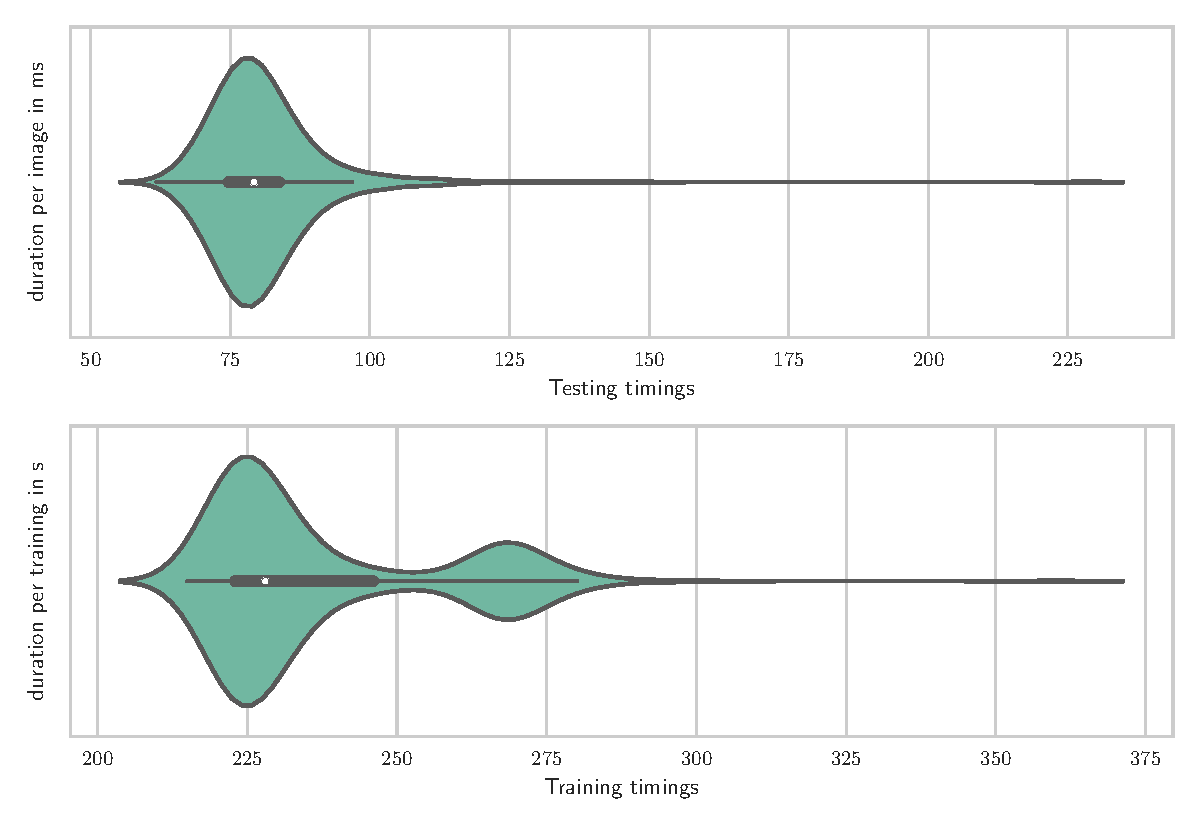
\includegraphics[width=0.9\textwidth]{figures/timings_fig}
  \caption{Distribution of durations in testing and training. Time in training measured in seconds for training over 500 iterations. Time in testing is measured in ms per image completing forwarding and all postprocessing.}
  \label{fig:timings}
\end{figure}
For the application of this method in a live production setting, speed is from huge importance. Therefore we measure and report the duration for training and deployment of the network \fref{fig:timings}. Training takes around 3.5 minutes on a single Titan X and testing runs at around 55ms per image. With therefore approximately 18 images / second we are reaching real-time search in image databases.\\
Although this is a short time for a train and test run of a neural network it  nevertheless does reduce the applicability of this approach. If we assume an art image database of 10.000 images, a query and complete search through the database would take $t \approx \SI{210}{\second} + \sfrac{10000}{18}s = \SI{12.8}{\minute}$.

There might be options to improve the time performance. One idea is to precompute the last feature maps for all images, so that, while searching through the images, we only have to compute a single convolution and the bounding box retrieval. This might drastically improve retrieval speed but training the network still causes a practical barrier.
